\documentclass[oneside,phd,10pt]{ucl_thesis}

\usepackage{url}
\usepackage{hyperref}
\hypersetup{pdfborder={0 0 0}}
\usepackage[printonlyused]{acronym}
\usepackage{textcase}
\usepackage{graphicx}
\usepackage{epsfig}
\usepackage{amssymb}
\usepackage{amsmath}
\usepackage{amsfonts}

\usepackage{caption}
\usepackage{subcaption}
\usepackage{verbatim}

\usepackage{color}
\usepackage{array}
\usepackage{multirow}
\usepackage{listings}
\usepackage{booktabs}

\hypersetup{
colorlinks,
citecolor=black,
linkcolor=black,
urlcolor=black
}
\newcolumntype{$}{>{\global\let\currentrowstyle\relax}}
\newcolumntype{^}{>{\currentrowstyle}}
\newcommand{\rowstyle}[1]{\gdef\currentrowstyle{#1}%
  #1\ignorespaces
}
\newcommand{\ra}[1]{\renewcommand{\arraystretch}{#1}}

\lstset{language=C}

\newtheorem{definition}{Definition}[chapter]
\newtheorem{theorem}{Theorem}[chapter]

\newcommand{\chapfolder}{chapters}
\newcommand{\locfolder}{}

\newcommand{\Esym}{\text{E}}
\newcommand{\E}[1]{\Esym\left[#1\right]}

\includeonly{\chapfolder/introduction,
             \chapfolder/resourcepooling/all,
             \chapfolder/preflex/all
             \chapfolder/appendixa
}

\newcommand{\COMMENT}{\color{red}}
\newcommand{\LOREM}{{\color{blue} Lorem ipsum dolor sit amet, consectetur adipisicing elit, sed do eiusmod tempor incididunt ut labore et dolore magna aliqua. Ut enim ad minim veniam, quis nostrud exercitation ullamco laboris nisi ut aliquip ex ea commodo consequat. Duis aute irure dolor in reprehenderit in voluptate velit esse cillum dolore eu fugiat nulla pariatur. Excepteur sint occaecat cupidatat non proident, sunt in culpa qui officia deserunt mollit anim id est laborum. }}

\title{Traffic re-engineering:\\[1em] {Extending resource pooling through the application of re-feedback}}

\author{Jo\~{a}o Taveira Ara\'{u}jo}
\date{2014} %The date on the copies of the thesis submitted for examination in November and December should be that of the following year.
\begin{document}
\maketitle

\newpage

\hphantom{}\vfill
\thispagestyle{empty}

%\noindent {\large{Examination Committee:}}\\

%\noindent {\large{External Examiner, Affiliation}}\\

%\noindent {\large{Internal Examiner, Affiliation}}\\

%\noindent {\large{Dr George Pavlou, University College London}}\\

\noindent {\small{I, Jo\~{a}o Taveira Ara\'{u}jo, confirm that the work presented in this thesis is my own. Where information has been derived from other sources, I confirm that this has been indicated in the thesis.}}\\

\par\noindent\makebox[2.5in]{\hrulefill}

\noindent {\small{\copyright\ 2008--2014, Jo\~{a}o Taveira Ara\'{u}jo}}\\

\noindent {\small{Department of Electronic \& Electrical Engineering\\University College London}}

%\pagenumbering{roman}
% Abstract
\begin{abstract}
\addcontentsline{toc}{chapter}{Abstract}

Parallelism pervades the Internet, yet efficiently pooling this increasing path diversity has remained elusive. 
With no holistic solution for resource pooling, each layer of the Internet architecture attempts to balance traffic according to its own needs, potentially at the expense of others.
From the edges, traffic is implicitly pooled over multiple paths by retrieving content from different sources.
Within the network, traffic is explicitly balanced across multiple links through the use of traffic engineering.
This work explores how the current architecture can be realigned to facilitate resource pooling at both network and transport layers, where tension between stakeholders is strongest.

The central theme of this transfer is that \emph{traffic engineering} can be performed more flexibly, efficiently and robustly through the use of \emph{re-feedback}.
A mutualistic architecture is proposed enabling resource pooling to be performed both by hosts, who can exploit greater path diversity, and the network, which gains insight into properties of traffic currently only visible at the transport layer.
A congestion balancer is derived which provides resilient and efficient pooling even in the absence of multipath transport.
Opportunities for harnessing the changing properties of Internet traffic are then identified through a longitudinal measurement study of interdomain traffic spanning five years.

All of the above represent concerted attempts to rethink and reassert traffic engineering in an Internet where competing solutions for resource pooling proliferate.
By delegating responsibilities currently overloading the routing architecture towards hosts and re-engineering traffic management around the core strengths of the network, the proposed architectural changes allows the tussle surrounding resource pooling to be drawn out without compromising the scalability and evolvability of the Internet.


\end{abstract}


\begin{acknowledgements}
\addcontentsline{toc}{chapter}{Acknowledgements}
%The resulting interactions between congestion control and traffic engineering are not easily understood, and have led to a more opaque and convoluted Internet.


%In this paper we debate existing approaches to resource pooling and present PREFLEX, an architecture where edge networks and hosts both share the burden and reap the rewards of balancing traffic over multiple paths. 
%Using PREF (Path RE-Feedback), networks suggest outbound paths to hosts, who in turn use LEX (Loss Exposure) to signal transport layer semantics such as loss and flow start to the underlying network. 
%By making apparent network preferences and transport expectations, PREFLEX provides a mutualistic framework where congestion control and traffic engineering can both coexist and evolve independently.
%

%In particular such a system must rarely reorder packets, must not require per-flow state, must cope with different paths having different bandwidths and must be self-tuning in a variety of network contexts. 
%
%
%This paper argues there is a need to rethink the current traffic management architecture to involve both network and transport layer, allowing end-host congestion control and network traffic engineering to become aware of each other. 
%Only by fomenting cross layer cooperation will traffic management be able to provide the robustness and performance required for the future Internet without compromising its scalability and capacity for innovation.
%

\end{acknowledgements}


\newpage

\tableofcontents

\listoffigures
\addcontentsline{toc}{chapter}{List of Figures}

\listoftables
\addcontentsline{toc}{chapter}{List of Tables}

%%\pagenumbering{arabic}
%%\setcounter{page}{1}

\chapter{Introduction}
\label{sec:introduction}

% resource pooling
Strategies for pooling traffic are locally applied by all stakeholders on the Internet in a bid to improve efficiency, resilience and flexibility.
Operators resort to traffic engineering to load balance traffic across available network resources. 
Hosts adapt their sending rates to probe available network capacity.
\ac{P2P} applications often retrieve data chunks from multiple locations in order to efficiently distribute content amongst peers.
Content providers can manipulate name resolution to balance demand across servers and hosting infrastructure.
While these mechanisms share similar goals, they do so from different perspectives and as such may be at odds with each other.

% towards multipath transport
This antagonism is played out within the Internet architecture as network, transport and application layers all attempt to influence how and where traffic flows.
Against a backdrop of significant shifts in traffic patterns \cite{Cho:2006p104,Cho:2008p488} and greater path diversity \cite{Teixeira:2003p132,Bennett:1999p120,Oliveira:2006p342}, the issue of how best to balance traffic across multiple paths has become more relevant over time.
Bolstered by strong theoretical groundwork \cite{Kelly:2005p140,Key:2007p130}, support for enshrining traffic balancing at the transport layer has gained momentum, leading to recent efforts in the standardization of multipath transport \cite{Ford:2011p490}.
The deployment of such protocols however is likely to be hindered by an operational reality; namely that most path diversity is within the network, and that most providers are unwilling to relinquish control of how traffic traverses their networks.

% the network is not enough
The network alone on the other hand appears incapable of managing traffic efficiently.
For one, operators are constrained to balancing traffic transparently due to end host expectations.
On the other hand, routers do not have enough knowledge of end-to-end traffic to make informed decisions on which path each packet should take.
In many cases operators have enhanced their ability to manage traffic by extracting additional information per-packet, by looking beyond the network header, and per-flow, by reconstructing data streams over time, both of which engrain protocol specific behaviour into the network.
This increase of network awareness however comes at the expense of innovation at the edges, as developers become increasingly constrained in what type of protocols can be deployed.

% join both?
Whether applied to providers wishing to reduce costs or hosts attempting to maximize throughput, the proliferation of unilateral solutions for resource pooling are manifestations of an underlying need. 
Rather than confine resource pooling to a single point of the Internet architecture and risk alienating a subset of stakeholders, this thesis explores how the existing Internet architecture can be extended to accomodate both host and network requirements for resource pooling.

\section{Problem statement}
\label{sec:introduction:objectives}

This thesis attempts to answer the following question:

\begin{quote}
\textit{
Given the nature of Internet traffic, how can the current architecture be realigned to facilitate resource pooling at both network and transport layers?
}
\end{quote}

In proposing to \emph{realign the current architecture}, the emphasis of any proposed solution must be applicable to the existing Internet architecture.
The motivation for avoiding clean-slate solutions was largely due to the nature of the problem at hand.
The different forms of resource pooling which we are attempting to reconcile are a product of both the Internet architecture and its stakeholders.
While it is clear that a clean-slate approach to resource pooling would have resulted in a different architecture, it may also have given rise to different stakeholders or different traffic patterns.
By adhering to existing protocols, any potential solution can be directly applied and, by extension, validated. 

While resource pooling is prevalent across all layers, the focus of this work is mostly restricted to reconciling \emph{network} and \emph{transport} layers. 
Most forms of resource pooling above the network layer will attempt to benefit the end user, while below the transport layer most resources within a single administrative domain will conspire towards the same ends.
It is at the intersection of network and transport layers where the juxtaposition of interests is greatest within the Internet architecture.

By \emph{facilitating resource pooling} however, we do not expect to dictate an outcome to the tussle between network and hosts, but rather provide an architecture within which such a tussle can evolve.
In some cases balancing traffic solely from the hosts may be desirable, while in other cases providers may wish to retain full control.
Both represent extremes of a range of outcomes which should be possible within a unifying architecture.

Finally, designing an efficient resource pooling architecture must take into account the \emph{nature of Internet traffic}.
While scaling Internet traffic poses considerable technical challenges, understanding its emergent properties plays a pivotal role in simplifying traffic management.
Any solution presented must not only address future traffic needs but also exploit its properties.

\section{Contributions}

The first contribution of this thesis is to propose a \ac{PREFLEX} architecture for \emph{mutualistic} resource pooling.
\ac{PREFLEX} bridges different forms of resource pooling by exposing path diversity to hosts and making the network aware of traffic characteristics which are crucial to effective traffic engineering.

Secondly, a traffic balancer is derived which enables providers to balance congestion rather than load.
Congestion balancing mimics the way in which multipath transport protocols spread their traffic across links and represents one possible instantiation of \ac{PREFLEX}.
Balancing congestion from within the network not only benefits flows which are not multipath enabled, but also improves resilience by keeping minimal network state on tracking performance across different paths.

The third contribution is a publicly available dataset, \ac{MALAWI} providing information on the end-to-end characteristics of approximately 5.7 billion TCP data flows collected over five years, and how they relate to their topological and geographical endpoints. The collection and aggregation of flow-level metrics by location over time can provide valuable insight in two key areas. Transport-level information can assist in understanding how TCP behaves: both by tracking how endpoints perceive network performance, and how the protocol is evolving. This can potentially not only assist in protocol design improvements, such as evaluating the adequacy of TCP parameters \cite{Dukkipati:2010p160}, but also in evaluating how widely deployed particular elements of TCP are. Additionally, observed traffic is mapped to the underlying routing system, which can be of value in topics as varied as fragmentation of address space \cite{Cittadini:2010p431}, FIB aggregation \cite{Ballani:2008p199} or informing caching strategies \cite{Psaras:2011p487}.

The final contribution is in using the resulting dataset to attempt to shed light on three fundamental questions: where is traffic flowing, with what characteristics and how has this changed over time? This information is critical in understanding how the characteristics of traffic can be harnessed to manage traffic through simpler and more flexible means.



\section{Publications}
\label{sec:introduction:contributions}

\begin{itemize}
    \item J. Taveira Ara\'{u}jo, R. Landa, K. Fukuda and G. Pavlou. \\
            \emph{A longitudinal analysis of Internet traffic} \\
            Under submission.
    \item J. Taveira Ara\'{u}jo, K. Fukuda. \\
            \emph{MALAWI: Aggregated longitudinal analysis of the MAWI dataset} \\
            {ACM CoNEXT Student Workshop 2011}
    \item J. Taveira Ara\'{u}jo, I. Grandi, R. G. Clegg, M. Rio and G. Pavlou \\
            \emph{Balancing by PREFLEX: Congestion Aware Traffic Engineering} \\
            {IFIP Networking 2011}
    \item J. Taveira Ara\'{u}jo, M. Rio and G. Pavlou \\
        \emph{A mutualistic resource pooling architecture} \\
        {ACM ReArch 2010}
    \item T. Moncaster, L. Krug, M. Menth, J. Ara\'{u}jo, S. Blake, R. Woundy \\
        \emph{The Need for Congestion Exposure in the Internet} \\
        {draft-moncaster-conex-problem-00, IETF Internet draft 2010}
\end{itemize}

\section{Thesis Outline}
\label{sec:introduction:outline}

This thesis is organized as follows.
Chapter \ref{sec:resourcepooling} provides an overview of how resource pooling is performed across different layers of the Internet architecture.
Chapter \ref{sec:preflex} introduces a mutualistic resource pooling architecture, while chapter \ref{sec:cate} explores how such an architecture can be exploited by providers wishing to balance congestion rather than traffic.
Chapter \ref{sec:malawi} details a measurement study to characterize the evolution of Internet traffic.
Finally, chapter \ref{sec:conclusions} presents the roadmap for future work and preliminary conclusions.


\chapter{A longitudinal analysis of \acs{TCP} traffic}
\label{chapter:malawi}

\renewcommand{\locfolder}{\chapfolder/malawi}
\section{Introduction}

% generic "failures are bad"
Despite being broadly designed for robustness, the current Internet architecture remains remarkably vulnerable to failures.
Managing faults effectively poses a significant operational challenge, in part because faults differ widely in both source and nature, potentially occuring at any layer of the stack and along any element along a path.

% neither is transport
\LOREM
\LOREM

% network methods
Given the commercial nature of the Internet, the onus of providing resilience has instead shifted to network operators.
Traditionally this has been achieved by overloading the routing architecture.
The deployment of real time applications with harder constraints on reliability coupled with better failure detection methods embedded in linecards have provided both the motivation and the means for achieving sub-second recovery within IGP networks \cite{}.
Even with reduced recovery times however, the transient effects of routing changes can still disrupt the forwarding path. 
Under such cases diverse proposals such as Fast Re-Route \cite{}, Loop-Free Alternate next hops \cite{} or Packet Re-cycling \cite{} can provide repair paths for use between the detection of a failure and the convergence of the routing process.

Unfortunately, such methods are rarely sufficient.
Firstly, their application is circumscribed to individual domains, and as such cannot provide end-to-end coverage in a federated, best-effort Internet.
Secondly, there are many faults which do not directly pertain to routing, such as middlebox misconfiguration or hardware malfunctions, and as such go undetected.
Finally, reparation often disregards and potentially disrupts the transport layer by causing out-of-order delivery of packets.

% why now. datacenter, SDN
\LOREM
\LOREM
\LOREM

% layout?
\LOREM
\LOREM


%Outside their networks however, operators are reduced to negotiating service level agreements with their own providers who are invariably unable to cater for such specialized demands \cite{}.
%Even if such terms were met, the Internet architecture provides limited visibility beyond one's own domain.
%This opaqueness, in addition to the fact that failures themselves may be distributed in nature \cite{}, severely limits the ability for a customer network to trace remote problems to a single source \cite{}.
%With no means to hold providers accountable for failures, there is little to enforce the terms of a truly end-to-end SLA.
%
%Unfortunately, such intradomain methods 


%Alongside this increased centralization of resources comes a heightened sense of accountability.
%The commercial nature of the agreements between customers and cloud hosting companies such as AWS \cite{} often involve the establishment of service level agreements.
%Even where such agreements are not explicit, such as the base option of tiered services such as Dropbox or Heroku, there is an inherent need to minimize the impact of outages -- non paying customers may be less demanding, but they are also less sensitive to the switching cost incurred in changing service provider.
%
%Unfortunately, the federated, best-effort nature of the Internet seemingly does not lend itself to such high expectations.



%Under such cases, a network operator is currently expected to detect, repair and recover from such faults.
%Detection often requires scale -- the reliability with which a fault can be identified relies on the proportion of traffic affected. 
%In many cases, faults affecting single flows may go undetected by the network.
%Once detected, reparation varies according to the nature and origin of the fault.
%For some cases, such as intradomain routing, this process is often automated and robust.
%For many others however, such as faulty hardware or misconfigured devices, recovery is difficult and error-prone.
%In either case, the amount of time expended in detection and repair can often preclude recovery, since most flows will terminate after successive timeouts.
%

%Fueled largely by economies of scale in both software management and hardware acquisition and maintenance, the emergence of cloud computing and content distribution networks has lead to a profound shift in Internet traffic.
%
%
%Whereas the advent of broadband connections init
%In contrast to the highly distributed nature of peer-to-peer software which 
%
%
%For one, never has so much been distributed by so few to so many.
%% AS dist graph
%% netflix
%
%\LOREM
%
%% Accountability, resilience

%All intervening equipment is subject to failure along a network path, with recovery time depending not only on \emph{what} happened, but also \emph{where}.
%Within their networks, operators are free to instrument and deploy arbitrarily complex tools to meet requirements. 
%This freedom has lead to a proliferation of proposed improvements in resilience for intradomain settings \cite{}.


%The establishment of SLAs for network availability have traditionally been prefered within the telecom industry in particular, and represent one possible approach to ensuring resilience. An alternative approach is offered by the end-to-end principle. 
%Since end hosts possess both inherent knowledge of application needs and fine-grained measurements on end-to-end path characteristics, the transport layer is often identified as a more natural fit for dealing with fault tolerance at an Internet scale.
%Both SCTP \cite{} and MPTCP \cite{} enable transparent fail-over through multihoming.
%In spite of providing significant features, neither is likely to be widely deployed in the near future: the former lacks critical middlebox support, while the latter is still undergoing standardization.
%Furthermore, the requirement for end-host multihoming has also posed a barrier to deployment.
%Finally, all transport approaches to fail-over confine knowledge of faults within an individual flow: each flow must detect failures independently, even when many flows are affected by the same fault.
%


% Transport is not the answer

% Can we do better with SDN?


%A default forwarding plane, corresponding to the label 0, must be defined and cater for all traffic destinations.
%As with existing routing infrastructure, this single default plane will suffice for most traffic.

%Invariably however, path failures will arise which may affect any number of flows.
%Rather than expecting the network to address end-to-end failures, hosts are allowed to proactively request an overlay plane from the network.





\section{Related work}
\label{section:malawi:related}

Despite their inherent value, longitudinal studies of Internet phenomena are rare. 
Over its short lifespan the Internet has been shaped as much by technological change as by political and commercial realities. 
This dynamic nature does not lend itself to observational studies where data must be collected and curated over long periods of time, and has resulted in a scarcity of relevant datasets. 
What few exceptions exist often stem from collaborative research efforts, such as CAIDA \cite{CAIDA} or Oregon Routeviews \cite{routeviews}. 
The usefulness of these datasets however can be severely affected by the need for data privacy. 
The dissemination of interdomain routing information, where no such requirement exists, has assisted in a wealth of research on wide ranging topics, from quantifying path diversity \cite{Oliveira:2009p203} to locating Internet bottlenecks \cite{Hu:2004p96}. 
In contrast, longitudinal datasets relating to passive measurements have nurtured a much smaller community of researchers often focusing on characterizing traffic \cite{Fontugne:2010p413}. 
Stripped of the locality contained within IP addresses however, researchers are left unable to relate these findings to a wider context.
Instead, cross-sectional studies characterizing traffic aggregated by location are frequently conducted under different contexts \cite{Ager:2011:WCC:2068816.2068870}, but lack the temporal perspective only longitudinal studies can afford. 
Efforts to characterize the spatial properties of traffic over time \cite{Dhamdhere:2011p428,Labovitz:2010:IIT:2043164.1851194,Cho:2008:OSC:1544012.1544024} have defined the changing of Internet topology and traffic alike but fall short of relating such shifts with their impact on relevant metrics such as loss or delay. 

% other work since
This chapter builds on a wealth of prior work on understanding Internet traffic and serves as a reappraisal of significant past contributions.
Flow characteristics and \ac{TCP} behaviour at large are subject to frequent reassessment \cite{Zhang:2002p85}.
Of particular relevance to the current work are passive studies which delve into the inner mechanisms of \ac{TCP}.
In \cite{Jaiswal:2004p242}, Jaiswal et al.\ infer the sender's congestion window by identifying the congestion control variant from the behaviour observed during loss recovery.
The use of separate state machines for each variant however proves unscalable given the many flavours of \ac{TCP} congestion control which have since been deployed.
In \cite{Lan:2006p566}, Lan et al.\ analyse flows according to size, duration, rate and burstiness and characterise the observed correlations for heavy-hitters specifically,
uncovering evidence of increased application influence on flow rates and burstiness and consequently suggest treating flow size and duration as independent dimensions.

One central aspect to the analysis of \ac{TCP} behaviour is the estimation of \ac{RTT} from packet capture data. 
In addition to SYN-based methods, Shakkotai et al.\ \cite{Shakkottai:2004p408} evaluate further techniques to estimate the \ac{RTT} of a unidirectional flow. 
The \textit{rate change} method establishes a relation between the \ac{RTT} and the increase in sending rate, assuming linear window increases during congestion avoidance. 
Unfortunately, this assumption no longer holds, both due to the proliferation of less conservative congestion control algorithms such as CUBIC \cite{Ha:2008p471}, and due to application-driven flow control. 
An alternative is the use of frequency-domain techniques \cite{Veal:2005p412,Lance:2005p565,Qian:2009p429}, which are a natural fit given the self-clocking nature of \ac{TCP}. 
However, a common difficulty with the application of spectral analysis is extracting the fundamental frequency which corresponds to the \ac{RTT} in the presence of noise. 
In applying the Fourier transform to inter-packet arrival times, for example, Qian et al.\ \cite{Qian:2009p429} note that less than half of all flows have distinguishable \textit{flow clocks}; likewise, the \ac{FFT}-based \ac{RTT} recovery was found to be unreliable even after pre-processing available data to enhance inherent periodicities.

% topological influence
Finally, it is important to elucidate what changes in traffic properties are intrinsic to \ac{TCP} and data transfer, and which ones arise from large-scale changes in the \ac{AS}-level topology of the Internet. 
In the decade since publication of \cite{Zhang:2002p85}, the Internet has undergone significant changes, shifting from a broadly hierarchical form to a flatter, more interconnected structure \cite{Labovitz:2010p175,Ager:2012p567}.
Given the longitudinal nature of this chapter and its focus on interdomain traffic in particular, the insights provided by these studies on the macroscopic effects of content consolidation are discernible within the studied dataset, and as such are a source of validation for many of the observations herein.

\section{Dataset}
\label{section:malawi:dataset}

This section provides an overview of the datasets used in this work and some of the data processing required before approaching the longitudinal study of Internet traffic rate limiting. We use the original, unanonymised traffic traces of the MAWI \cite{mawi} dataset, a set of daily traces from the WIDE backbone network which provides connectivity to universities and research institutes in Japan. Traffic is captured daily for 15 minutes starting at 14:00JST. Although this dataset extends back largely uninterrupted from late 2001, we focus on just over five years of data following a network upgrade to the monitored link on October 2006.

The monitored link carries mostly trans-Pacific commodity traffic between WIDE customers and non-Japanese commercial networks. 
We will refer to traffic towards WIDE as \emph{inbound} traffic, whereas traffic originating from within WIDE is referred to as \emph{outbound} traffic.

\begin{table}[!htp]
\scriptsize
\centering
    \begin{tabular}{r|cccccc}
        & & TCP data & \multicolumn{2}{c}{Traffic (TB)} & \multicolumn{2}{c} {Count ($\times10^3$)} \\
        Year & Days & flows (x$10^6$) & In & Out & AS & Prefixes \\
        \hline
        2006 & 91 & 20.52 & 0.43& 0.45 & 10.90 & 56.86\\
        2007 & 350 & 102.56 & 2.11 & 2.49& 17.21 & 113.79\\
        2008 & 358 & 112.26& 2.43 & 2.10& 24.74 & 156.54\\
        2009 & 364 & 113.97& 2.48 & 2.53& 19.71 & 143.87\\
        2010 & 365 & 113.70& 2.58 & 3.43& 20.38 & 148.03\\
        2011 & 358 & 114.74& 3.44 & 5.14& 19.99 & 140.56\\
        \hline
        Total & 1886 & 5777.55 & 13.50 & 16.14 & 34.12 & 341.22\\
    \end{tabular}
    \caption{\label{table:overview}Overview of traced MAWI dataset 
}
  \vspace{-3mm}
\end{table}

A preliminary overview of the dataset used is provided in table \ref{table:overview}. 
In total, 5.7 billion flows containing data are traced over five largely uninterrupted years; this represents approximately 30 terabytes of TCP traffic. For the purposes of this work, we will focus exclusively on inbound traffic, 60\% to 80\% of which originates from port 80, referring only to analysis of outbound traffic when providing a wider context for our findings.
Given the sender side plays a critical role in shaping traffic, analysing traffic for which the source is restricted to a small set of networks within Japan would be of limited use in accurately depicting traffic trends at large.
We instead fix hosts within Japan as sinks, thus sharing a similar perspective on inbound traffic as many other networks. 

\subsection{Tracing TCP Metrics}

All TCP flows are reassembled and analysed for each daily trace.
In addition to the five tuple used to define each connection, we impose two additional restrictions: a contiguous sequence number space and a three minute timeout. These restrictions are helpful to deal with port reuse and unterminated flows respectively.  
Although the total number of TCP flows increased dramatically in 2011, the number of flows \emph{for which data payload was seen} has remained stable, averaging over 100 million data flows traced per year.  

There is much prior work with regards to reconstructing TCP flow from passive measurements and using this information to understand the end-to-end properties of traffic \cite{firstRTT,Jaiswal:2007p233,Rewaskar:2007p195,Shakkottai:2004p408}. However, the MAWI traces impose two constraints which require careful consideration, and ultimately led to the use of a custom TCP tracer. 
The first one is the proportion of bidirectional flows, that is flows, where both forward and reverse path are seen. 
In the dataset used this fluctuates between 40\% and 60\% over five years.
Most available TCP tracers either ignore or are inadequate at processing unidirectional flows. 
The second one is the short duration of each individual trace file. 
At only 15 minutes of line-rate data capture per day, it is wasteful to ignore flows which are not complete. Although the number of flows for which a SYN and FIN in either direction is observed has remained consistently high until late 2011, these flows are normally \emph{mice}, i.e. flows that tend to be brief and which carry little traffic individually. In contrast, most \emph{elephants} (flows that carry significant traffic individually) have durations that exceed that of each trace file. 

%rtts traced
%While many metrics are extracted for each flow, for the purposes of this paper we will focus only on detailing how we collected delay and loss.
%Passive RTT estimates, calculated as the offset between a data packet and its respective acknowledgement, require both directions to be observed at the measurement point. 
%This provides delay estimates between the measurement point and the receiver, as illustrated in figure \ref{fig:synrtts}. 
%For flows where data is transfered in both directions, we will obtain in effect two separate estimates, $RTT_{m2a}$ and $RTT_{m2b}$, illustrated in figure \ref{fig:synrtts}. 
%Together they form the total end-to-end delay experienced by end-hosts. 
%For the remainder of this paper, the term RTT will refer to delay between our measurement and destinations outside WIDE. 
%We discard the delay between measurement point and hosts within WIDE for two reasons. 
%It is both negligible for a large proportion of traffic, which is highly concentrated within the Tokyo metropolitan regions and immediate surroundings, and extremely large for a very small subset of hosts located outside Japan, as WIDE has in the past acted as a provider to academic institutions in Indonesia through a satelite uplink. 
%By decoupling both directions we focus purely on the changes in delay to locations outside Japan. 
%This incurs a reduction in the range of destinations for which we can obtain estimates - only bidirectional traffic can be traced this way. 
%For the set of destinations we will study in this paper, we shall show that this reduction is small. 
%For tracking delay changes for unidirectional traffic for other purposes, MALAWI includes RTT estimates extracted from the SYN exchange.

Loss is inferred by accounting for \emph{retransmissions} in the upstream data and \emph{out-of-order packets} in downstream data; for the remainder of the paper we will refer to the \emph{end-to-end loss} as the sum of out of order and retransmitted data bytes over the total data bytes in a given direction.
% XXX: remove RTT ref?
%Tracking both retransmissions and out-of-order packets accurately requires a reliable RTT estimate, which can only be obtained for bidirectional flows. We forfeit some precision by not taking this into account, as we wish to be consistent in how we estimate both metrics independently of the type of flow and aggregation. 
Pragmatically, we found this to be an adequate indicator of loss --- with the exception of \emph{hanging} TCP connections. 
In these cases where connectivity is lost, a host will proceed to retransmit packets while performing an exponential backoff. 
Although this results in negligible overall traffic, it can significantly skew the inferred loss ratio for uncommon destinations for which little traffic exists. 
To account for these cases, we imposed a 3-second timeout on retransmissions after which we consider the congestion feedback loop to be broken. 

Each daily trace in the dataset is processed from a packet level capture into a collection of flow level statistics. 
This gives us insight into the end-to-end characteristics of traffic. However, since a core objective of this work is to augment this time-based information with data describing the endpoints of each flow, aggregating by location is also required. 

\subsection{Aggregating by Location}

Location information is added by mapping the original source and destination IP addresses to its geographical and topological counterpoints. 
We use the \emph{routeviews} archives to reconstruct the mapping between each IP and both AS and network prefix; bi-hourly dumps of BGP RIBs are available in the WIDE archives since mid 2003. 
We reconstruct a daily RIB based on the views provided by contributing ASes, in particular IIJ and APNIC. 
Since exact routes are not disclosed (there is no record of local policy), we have no knowledge of the route taken by packets; this of course does not hinder our ability to consistently map IPs to ASes. While discrepancies in AS destinations exist between different routeviews contributors, we note that this happens almost exclusively on prefixes for which no actual traffic is seen. 

Mapping IP to country is done through the use of GeoLite \cite{maxmind}, a commercial geolocation database. 
While the accuracy of this solution is often disputed, we are not overly concerned with locating traffic at a fine granularity. 
We will mostly focus on tracking traffic by country and, for larger countries such as the U.S, by region, in order to capture shifts over time.
GeoLite proves adequate on both counts.
The archive for geolocation data only extends to 2009, before which we must rely on the earliest match. 
Additionally, we verify if the destination or source AS have maintained the same administrative mapping up until mid 2009 in the relevant RIR (regional internet registry) archives; otherwise, we do not associate a flow to a geographical location.
% bridging paragraphs to save space.
After associating flows to country, region, AS and network prefix for both source and destination IPs, we aggregate flow statistics over each location identifier. 
This generates a daily collection of location identifiers and associated flow properties, from which we can sketch the geographic and topological properties of the dataset over time.

\section{Methodology}

Providing a macroscopic view on where traffic originates from, and in what quantity, can be achieved by simply binning packets into flows and accumulating byte counts over geographical or topological locations. 
Uncovering application layer characteristics (i.e. \textit{how} traffic is sent) is a more complex problem that requires additional methods to reverse engineer transport behaviour.
The aim of this section is to describe a process which distinguishes those flows which have their throughput limited by mechanisms other than the usual \ac{TCP} response to loss and delay.
Each flow can be characterized as being either application paced, in which the sending application is limiting the data provided, host limited, whereby local constraints at either end host cap throughput, or receiver shaped, in which an artificial constraint is imposed by either a middlebox or receiver.

The classification proceeds in stages. 
Before classification, it is necessary to reconstruct the RTT of the flow if the flow is not bidirectional.  
This is achieved in section \ref{subsection:malawi:PeriodicEnhancement}. 
Because the sender's TCP state machine cannot be directly observed it is necessary then to estimate the size of the congestion window by observing the number of unacknowledged bytes in flight (\textit{flight size}).
This reconstruction is described in section \ref{subsection:malawi:flightAggregation} and provides the basis for flow classification. 
Flows are then checked in turn to see if they are application paced, host limited or receiver shaped and classified as belonging to the first of these classes for which they fulfill the necessary conditions.
Flows in none of these classes are either limited only by the network (delay or loss conditions) or are insufficiently large to trigger any further constraints.

\subsection{RTT Estimation}
\label{subsection:malawi:PeriodicEnhancement}

Building on prior work presented in section \ref{section:malawi:related}, this section proposes an algorithm that scalably recovers the RTT from one-directional traffic traces. 
% XXX: below implies microflights were used, but these aren't described (remove as appropriate)
Although \ac{RTT} estimation is a difficult problem, simplifying assumptions can be made.
For the \ac{MAWI} dataset most \acp{RTT} are relatively large, with the closest neighbouring country, South Korea, roughly 40ms away.
By only processing bidirectional traffic from Japan, the expected \ac{RTT} range can be reduced for all other traffic.
The recovery mechanism then enhances the natural periodicity of traces and scalably constructs flights associated with specific application and protocol behaviour.
In the following the mechanisms required by these two goals are described. 
%
% Why does this work?
%
In normal operation, many \ac{TCP} operations involve request-response cycles between two endpoints in which the \ac{RTT} $T$ provides a natural \emph{clock}.
Hence, the most natural way to estimate \ac{RTT} from \ac{TCP} traces is to correlate requests and responses exchanged in both directions. 
If only one direction of data is observed however, $T$ cannot be directly observed. 
Instead, it must be estimated from the way in which \ac{TCP} packets cluster in time due to the batching of request-response operations.

The \ac{TCP} \ac{cwnd} determines the number of unacknowledged bytes that a \ac{TCP} flow may maintain at any point in time. 
This can be referred to as \emph{bytes in flight} because they are in transit between the sender $S$ and the receiver $R$; an equivalent definition applies for the number of \emph{packets in flight}. 
Once $S$ has transmitted \ac{cwnd} data bytes, it will refrain from transmitting more until either some bytes are acknowledged by $R$ or \ac{cwnd} is increased by the sender. 
In the absence of losses, neither of these events can happen until a \ac{TCP} \ac{ACK} is received; this immediately reduces the number of unacknowledged bytes, but may also lead to a significant \ac{cwnd} increase (during e.g. \emph{slow start}). 
% XXX: number of unacknowledged bytes reduced, or CWND?
In the presence of losses, however, bytes can be re-sent if a packet is timed out and considered lost; in this case, the number of unacknowledged bytes is reduced.

%
% What is our main contribution, algorithmically speaking?
%
The main difficulty associated with one-sided TCP flow reconstruction is as follows.
Let $t_1, t_2, \ldots$ be a set of times at which packets $p_1, p_2, \ldots$ were observed at $S$ en route to $R$.
Suppose that a packet $p_j$ of size $b$ is observed at time $t_j$.
In addition, suppose that approximately one RTT $T$ later, the sender $S$ receives an ACK $a_j$ from $R$ for the $b$ bytes of $p_j$.
At this point, the TCP stack in $S$ will decrease the number of unacknowledged bytes by $b$, thus opening the possibility for sending additional traffic to $R$.
This can lead to another packet $p_k$ to be transmitted; let this packet be observed at time $t_k$ as it is sent towards $R$.
Assuming that processing delay is insignificant, the RTT experienced by $p_j$ can be approximated as $T \approx t_k - t_j$.
Now consider what happens if packets are only observed in the $S \rightarrow R$ direction.
Under such conditions, it is not possible to ascertain whether $p_k$ was sent explicitly as a result of $S$ receiving the unobserved \ac{ACK} $a_j$, or whether it was sent as a result of an \ac{ACK} $a_i$ associated with a previous packet $p_i$ rather than with $p_j$.
If, however, a packet $p_l$ is eventually observed that did result from the reception of $a_j$, the \ac{RTT} can be estimated as $T \approx t_l - t_j$ with $t_l > t_k$.
Following this same reasoning, approximately one \ac{RTT} later a packet $p_m$ will be observed for which $2T \approx t_m - t_j$; this can potentially continue for as long $S$ has data to send and $R$ continues sending \acp{ACK}.
This is the underlying reason that \ac{RTT}-related periodic regularities arise when considering the timestamps of observed packets \cite{Qian:2009p429}.

The reasoning above is at the heart of the proposed algorithm to improve \ac{RTT} recovery by enhancing packet stream periodicity. 
Assume that a packet $p_j$ is observed at time $t_j$. 
Considering the set $\mathcal{T}_j$ of all values of $\Delta t = t_k - t_j$ for every $k > j$, it is apparent that it will include estimates not only for the \ac{RTT} $T$, but also for all its multiples $2T, 3T, \ldots$ 
If $t_l-t_k \approx T$ and $t_k - t_j \approx T$ then it follows that $t_l - t_j = 2T$, and this value will also be included in $\mathcal{T}_j$. 

By maintaining a set $\mathcal{T}_j$ for every packet $p_j$ observed, at least some of its values will correspond to estimations of multiples of the \ac{RTT}. 
It then follows that by creating a set $\mathcal{T}$ that includes values calculated starting from every packet $p_j$ so that $\mathcal{T} = \cup_j \mathcal{T}_j$, numerous estimates for $2T, 3T, \ldots$ will also be included. 
Hence, the probability density function $H(t)$ of the values in $\mathcal{T}$ should show peaks around multiples of the \ac{RTT} (see Figure \ref{fig:histogram}). 

\begin{figure}
  \centering
  \includegraphics[width=0.8\textwidth]{figures/malawi/rttbin.pdf}
  \caption{$H(t)$ for flow displayed in Figure \ref{fig:hostlimited}. The horizontal line delimits $\overline{H}$ while the highlighted bin denotes the bidirectional RTT estimate.\label{fig:histogram}}
\end{figure}

%
% Explain why did we use FFT
%
The algorithmic recovery of $T$ from $H(t)$ presents additional challenges. 
In particular, $H(t)$ may include a large number of \ac{RTT} multiples, and a peak will be found for all of them. 
Crucially, all these peaks may be of comparable magnitude, complicating the task of selecting a single peak.
Moreover, these peaks need not be very pronounced, with histogram bins in close proximity of the peaks have very similar values as the peak itself. 
As such, taking \ac{RTT} candidates directly from $H(t)$ may result in a large set of similarly-valued bins situated around a peaks at multiples of the \ac{RTT}. 

Three recovery algorithms for $T$ are attempted.
First, as a baseline, the highest peak in $H(t)$ is selected as a candidate for $T$. 
In addition, expanding upon the work of Qian et. al. \cite{Qian:2009p429} a frequency-domain representation of $H(t)$ is used to identify $T$. 
This is done by selecting the highest peak of $|\hat{H}(\omega)|^2$, the \emph{energy spectral density} of $H(t)$ (i.e. the norm squared of the Fourier transform of $H(t)$). 
Finally, a custom utility-based technique that operates directly on $H(t)$ is proposed which achieves superior performance to both of the aforementioned methods.

%\subsubsection{FFT-Based RTT Recovery}
%We extract periodicity information from $H(t)$ by looking at $\hat{H}(\omega)$, the \emph{energy spectral density} of $H(t)$. Formally, $\hat{H}(\omega)$ is defined as the norm squared of the Fourier transform of $H(t)$, so that $\hat{H}(\omega) = |\mathcal{F}(H(t))|^2$. Using $\hat{H}(\omega)$ markedly improves the quality of our RTT estimation because the frequency peak corresponding to the RTT usually accounts for a much larger proportion of the total frequency domain energy than other peaks in $\hat{H}(\omega)$, leading to a much simpler discrimination of the true RTT. However, due to RTT changing during the lifetime of a flow, and also due to the expected noise associated with real-life data sources, $\hat{H}(\omega)$ can also occasionally include large peaks at frequencies unrelated to the RTT. In order to filter these out, we take a set of 10 frequency candidates from $\hat{H}(\omega)$, and use their associated periods as RTT candidates in our flow reconstruction algorithm (see Section \ref{
%subsection:malawi:flightAggregation}). We then select that RTT candidate which exhibits the smallest error, that is, that one which yields closest agreement with observed data.

%
% Algorithmic hacks
%
%To streamline our algorithm for streaming use, we use the following heuristics and approximations. Firstly, we define a range $[T_{\min}, T_{\max}]$ representing the range over which we find the RTT values of interest. Then, for each packet $p_j$, we build a subset $\mathcal{T}_j'$ of $\mathcal{T}_j$ by including all values of $t_j - t_k < T_{\max}$. We then generate $\mathcal{T}' = \cup_j \mathcal{T}_j'$ and approximate $H(t)$ by considering a histogram of the values in $\mathcal{T}'$. As usual, we do this by counting the frequency with which its values are observed in the ranges $[0,\tau)$, $[\tau, 2\tau)$, $[2\tau, 3\tau), \ldots$ where $\tau$ is the time resolution required. 


\subsubsection{Utility-Based RTT Recovery}
\label{sect:utilityBasedRecovery}

This method relies not on the identification of periodicities, but on explicitly matching experimentally found signatures. 
To this end, we consider the peaks of $H(t)$, which are then considered RTT candidates.  
However, trivial discriminators (such as simply selecting the highest peak) are not reliable. 
In this case, it was found experimentally that repeatable peaks and troughs also occur at multiples and sub-multiples of $T$, with the most important ones being $\frac{T}{3}$, $\frac{T}{2}$, $T$ and $2T$. 
We design this detection algorithm around the idea that a given pattern of peaks and troughs can identify $T$.

If we define $\overline{H}$ as the mean height of $H(t)$, we can define a per-peak utility function $p(t)$ so that 
\begin{equation*}
p(t) = 1.0 - \exp\left(-2.0 \left(\frac{H(t)}{\overline{H}}\right)\right) \mbox{.}
\end{equation*}
This function has several advantageous properties: it is 0 if $H(t)$ is zero, 1
if $H(t)$ is infinite, and $0.5$ if $H(t) = \overline{H}$.  In other
words it is a measure of the \emph{peakiness} of the data, with $p=1$ identifying
an infinitely high peak, $p=0$ identifying an empty histogram bin (trough), and $p=\frac{1}{2}$ 
implying that $H(t)$ is of exactly average height at that point. We can then score each candidate using the following utility function:
$$
P(t) = 1.5 p(t) + p(2t) - p\left(\frac{t}{2}\right) - p\left(\frac{t}{3}\right).
$$
That is, the candidate RTT $t$ scores highly if it is itself a peak, if it has a peak
at a multiple $2t$, and if it also manifests troughs at submultiples $\frac{T}{2}$ and $\frac{T}{3}$.
The factor of 1.5 was added after observations
showed that the peak at $T$ was the most important factor in determining
whether a candidate was the true RTT. Similarly, additional multiples and submultiples 
were excluded as they showed very limited discriminating power experimentally.

\begin{figure}
  \centering
  \includegraphics[width=0.8\textwidth]{figures/malawi/rttcomp.pdf}
  \caption{Accuracy of RTT estimator when compared to the median value of bidirectional estimate.}
\end{figure}

\subsubsection{Comparing RTT Recovery Algorithms}
\label{sect:comparingRecoveryAlgos}
As described in Section \ref{subsection:malawi:PeriodicEnhancement}, $H(t)$ is calculated in such a way that RTT periodicity is amplified. 
This means that FFT-based techniques could potentially perform better on $H(t)$ than on the packet stream with no pre-processing. 
However, this is complicated not only because $H(t)$ contains periodicities at multiples of $T$, but also discontinuities that generate harmonics at frequency multiples of the RTT fundamental. 
Hence, although the FFT $|\hat{H}(\omega)|$ of $H(t)$ is much cleaner than that of the packet interarrival time series on its own, its maximum peak rarely coincides exactly with the RTT clock (this corroborates reports by Qian et al \cite{Qian:2009p429}). 
Thus, applying the FFT leads to another \emph{peak detection problem} in which the RTT fundamental needs to be extricated from its harmonics and sub-harmonics. 
The trivial solution to this problem, the application of a bandpass filter around the RTT frequency, is of course unfeasible because the bandwidth and 
centring of such a filter depend on the RTT which is itself unknown.
The utility-based algorithm described in Section \ref{sect:utilityBasedRecovery} can hence be applied in either the time domain or the frequency domain; we chose to do it on the former on the interest of expediency and lower computational cost.

\newcommand{\RTTHeader}{Below & Above}
\newcommand{\SmallFlowName}{\textless 10MB}
\newcommand{\LargeFlowName}{\textgreater 10MB} 
\begin{table}
\footnotesize
\centering
\begin{tabular}{ p{1.5cm} p{1.2cm} p{0cm} p{.6cm}p{.6cm} p{0cm} p{.6cm}p{.6cm}}
& & & \multicolumn{2}{c}{Peak} & & \multicolumn{2}{c}{Utility-based} \\
\cline{4-5} \cline{7-8}
& Flow size & & \RTTHeader & & \RTTHeader \\
\cline{4-5} \cline{7-8} 
\multirow{2}{*}{Receiver side}  & \SmallFlowName && 4.31 & 9.13 && 4.58 & 6.35
\\ 
                                & \LargeFlowName && 6.72 & 6.43 & 4.97 & 5.33
\\
\multirow{2}{*}{Sender side}    & \SmallFlowName && 2.94 & 8.37 && 3.29 & 4.80
\\
                                & \LargeFlowName && 6.41 & 9.06 && 5.40 & 11.06
\\
\end{tabular}
\caption{\label{table:rttRecovery}Performance of RTT recovery algorithms}
\vspace{-3mm}
\end{table}

The performance of the analysed RTT recovery mechanisms is presented in Table \ref{table:rttRecovery}, that shows the percentage of total flows below and above the RTT range given by the bidirectional estimates.
We separate things for \emph{inbound} traffic (where we are positioned at the receiver side) and \emph{outbound} traffic (where we are positioned at the sender side). The utility-based algorithm is particularly useful to address RTT underestimation for flows over 10MB in size, which is our main objective since precisely that kind of estimation error would interfere with our ability to correctly decouple application behaviour from RTT-scale dynamics.


%For the most part, the utility based method improves on underestimation, which is our main objective since that would interfere with our flight reconstruction (i.e. generate lots of gaps).
%The exception (kind of) is traffic from the sender side, which in our training set (one week per year), had quite a lot of host limited traffic (paced out, no signal to recover).
%In this case, not a problem, since if the flow is long enough multiples of the RTT will still reveal host limitation, but will give us a smaller window..


\subsection{Flow Classification}
\label{subsection:malawi:flightAggregation}

One fundamental precondition to decouple the influence that network loss, host configuration and TCP behaviour has on the throughput experienced by a flow is the reconstruction of the congestion window behaviour of TCP flows on the basis of observed data. 
Unfortunately, the congestion window value is internal to the sender's TCP state machine and may not manifest itself in the absence of sufficient data from the application layer. 
A more easily observed quantity which serves as a reasonable proxy for the congestion window is the number of unacknowledged bytes in flight, henceforth referred to as the \textit{flight size}, which can be derived given an accurate estimate of the end-to-end delay.
The evolution of both flight size and RTT can in turn be used to ascertain to what extent throughput is regulated by limitations imposed at different layers of the networking stack.

% definitions
Given a candidate RTT, we can aggregate a stream of packets with arrival times $t_1, t_2, \ldots$ into a stream of \emph{flights}. 
Intuitively, a flight is a clustered subset of a TCP flow which exhibits its own temporal coherence; alternatively, it can be though of as a series of consecutive packets that were (roughly) generated by the sender as a response to the same protocol operation. 
A flight $f_i$ that begins
with the $j$th packet and ends with the $k$th is defined to have a \emph{total flight time} $\tau_i = t_{k+1} - t_j$. 
The algorithmic selection of initial and final packets in such a way that the resulting flights are indicative of TCP behaviour remains an open problem. 
Since we assume that the RTT provides a natural time frame for the operations of TCP, in the algorithm presented in this work, given an initial packet $\pi_j$ and an RTT estimate $T$, the $k$th (and final) packet is selected to minimise \emph{the flight time error} $e_i = |T - \tau_i|$. 
This mechanism follows closely the methodology described in \cite{Zhang:2002p85}, with the exception that we do not attempt to define flights as being both adjacent and disjoint; rather, we decompose flows into a stream of potentially overlapping flights. 
This helps the algorithm mitigate the deleterious effects of small deviations in the estimated RTT, which alters the properties of each flight. 
Furthermore, since the flight size is continuous in time, it makes little sense to restrict ourselves to a single sample per round trip time.

Having obtained flight information from each flow, we next consider what is the predominant factor that affects its throughput. 
Within the context of TCP, we classify flows as being artificially constrained by three distinct processes: \emph{application pacing}, \emph{host limited} and \emph{receiver shaping}.

\begin{figure}
\centering
  \centering
  \begin{subfigure}{1.0\linewidth}
    \includegraphics[width=1.0\textwidth]{figures/malawi/youtube.pdf}
    \caption{Application paced. \label{fig:youtube}}
  \end{subfigure}\\
  \begin{subfigure}{1.0\linewidth}
    \includegraphics[width=1.0\textwidth]{figures/malawi/hostflow.pdf}
    \caption{Partially host limited. \label{fig:hostlimited}}
  \end{subfigure}\\
  \begin{subfigure}{1.0\linewidth}
    \includegraphics[width=1.0\textwidth]{figures/malawi/awnd.pdf}
    \caption{Receiver shaped. \label{fig:awnd}}
  \end{subfigure}
  \caption{Flight size over time for flows affected by different artificial constraints. \label{fig:kindsOfFlowEffect}}
\end{figure}


\subsubsection{Application Paced Flows}
\label{sssec:app}

A flow whose throughput decreases because it has no outstanding data to send is temporarily limited by the application. 
Flights can be identified as being \emph{application limited} if terminated with a packet smaller than the maximum segment size (MSS) and followed by an inter-arrival time greater than the RTT, as consistent with \cite{Zhang:2002p85}. 
The underlying reason for this defintion is that most TCP implementations will wait some time for subsequent bytes to be written to the socket if the next packet to be sent is smaller than the MSS, unless the TCP\_NODELAY option is set \cite{nagle1984rfc}.

A flow with \emph{application limited} flights however is not necessarily \emph{application paced}. In practice, all flows for which the final packet is observed contain at least one such flight.
For the purposes of our work, we are focused on identifying cases in which throughput is predominantly determined by application behaviour.
One such example is illustrated in figure \ref{fig:youtube}, in which a stream is delivered by periodically writing blocks to the sending socket.
The resulting network-level behaviour is distinct from traditional congestion control: short bursts are interspersed with protracted silence.
Application limited flights, which terminate on non-MSS packets, are highlighted at the end of each burst.

This behaviour is in stark contrast to that exhibited in figure \ref{fig:hostlimited}, where distinct transfers are multiplexed on top of a single transport association over time.
From the perspective of the network, there is little to distinguish the behaviour of such traffic from independent TCP flows.
Application paced connections such as Youtube traffic however exhibit a degree of regularity which can potentially be exploited by the network in predicting demand or smoothing bursts.

In order to identify such recurring behaviour, we identify flows as being \emph{application paced} if the period between bursts terminated by \emph{application limited flights} is consistently under 10 seconds and the standard deviation of the intermediate pauses is under one second.
This definition in particular purposely ignores flows which exhibit long silence periods due to user interaction, and follows closely the behaviour historically associated to Youtube streaming in particular.

\subsubsection{Host Limited Flows}
\label{sssec:host}

Given sufficient bandwidth and traffic to send, a flow may encounter local constraints at either end-host which cap its throughput. 
For instance, the buffer space allocated on both the sender and receiver side is often pre-configured, and it is common practice to tune these values down on popular servers and managed infrastructure in a bid to conserve memory or bandwidth.
A receiver is also limited in the window size it can announce to the remote sender; if the windowscale option \cite{jacobson1992tcp} is not negotiated during the TCP handshake, the advertised window cannot exceed 64KB.

In both cases, a local decision by either host can determine the upper bound of the flow rate.
These \emph{host limited} cases are characterised by a constant window size over time.
The methodology described for flight aggregation at the beginning of this section typically generates a large number of flights, representing many likely combinations given a base RTT estimate.
In order to identify the flat-lined behaviour of a host limited flow, we first filter the flight stream to remove some of the uncertainty derived from small fluctuations in the RTT.
We then select the maximum flight size observed for each RTT interval, and declare a sequence of flights to be host limited if the same maximum was observed over six consecutive RTTs (this is twice the period suggested in \cite{Zhang:2002p85}).
In practice, increasing the period over which the maximum window size is tracked allows us to more accurately discern between host limited behaviour and more conservative bandwidth probing, such as that performed during the convex phase of TCP CUBIC \cite{Ha:2008p471}.

A flow may be host limited for only brief periods of its lifetime, as illustrated in figure \ref{fig:hostlimited}.
To filter out such cases where host limitations are not the predominant factor in defining flow throughput, we further enforce that in addition to host-limited flights, the average window size must over a flow lifetime should be within 10\% of the inferred host limit, which is not the case in figure \ref{fig:hostlimited}.

In practice, flows can exhibit both application pacing and host limitations, with bursts being sent at a capped window size followed by application pauses.
In such cases, a flow will still be classified as being \emph{application paced} if it meets the requirements set out in the previous section, as doing so provides evidence that it controls throughput in spite of the degraded performance provided further down the stack. 
This line of reasoning applies equally to the occurrence of sporadic loss; so long as block delivery is ensured within the timeframe dictated by the application, it remains in control.

\subsubsection{Receiver Shaped Flows}
\label{sssec:rec}

A flow which is neither \emph{application paced} or \emph{host limited} can still be artificially constrained by flow control (rather than by congestion control).
Traditionally, in TCP the sender is responsible for regulating throughput. 
However, the receiver can also shape throughput by manipulating the \emph{advertised window} announced on every acknowledgement.
Such receiver-window auto-tuning has been available on Windows operating systems since Vista \cite{vistaReceiveWindow}, and can also be leveraged by middleboxes in order to throttle inbound traffic \cite{appEx}.

In order to evaluate the potential impact of such behaviour, we further propose a heuristic to identify receiver-shaped traffic.
For flows in which both directions of traffic are observed it is possible to correlate the evolution of the advertised window with the size of reconstructed flights.
Figure \ref{fig:awnd} displays an example of a receiver-shaped connection, in this case throttled by an intermediate middlebox.
Since the advertised window may be fluctuating, it is not always obvious which of the many updates were effectively applied by the sender as successive values supersede each other.
An example of a reconstructed flow which is subjected to receiver shaping is displayed in Figure \ref{fig:awnd}.

For flows in which both directions are observed, it is possible to classify flights as being receiver-shaped if there is a statistically significant correlation between the advertised window size and the maximum flight size observed.
Harnessing the stream filtering used in detecting host limited behaviour, we perform such analysis over a sliding window of 10 RTT intervals.
A flight is flagged as being receiver shaped if the correlation between receiver window and flight size is statistically significant; a flow is considered to be predominantly receiver shaped if over half of its flights are flagged as such.
We do not perform this covariance analysis on flights which contain out-of-order or retransmitted packets. 
In these cases, both the receiver and sender window sizes are correlated \emph{by definition}. 
In the former case, the receiver buffer will temporarily fill expecting the next packet in sequence, in the latter case, TCP will reduce its window.

Given that receiver shaping classification requires correlating information in both directions of a TCP connection, it will come as no surprise that the absence of the reverse path can introduce false positives into our measurements. 
This happens because any given flow might be receiver shaped in such a manner that the heuristic erroneously attributes its behaviour to host limitations. 
In the absence of additional evidence, this misclassification is difficult to detect explicitly. 
Instead, we calculate the ratio of receiver shaped flows which would have been incorrectly identified if the reverse path were not observed. 
This error rate can then be used to evaluate the accuracy of classifier results.

\section{Performance Analysis}
%4.1) Balancing between two paths with high loss using fixed time unit
% using only loss-based balance in a simple regime where that works.
% Show how this converges quickly when one path suddenly gains
% background traffic (and hence loss).
%4.2) Balance between several paths with high loss and fixed time unit
% in simple regime where that works.
%4.3) Introduce experiment where equi-path is needed for probing and
% conservative is needed for low loss regime.
%4.4) Introduce experiment where time-scale tuning is needed to get
% good assessment of loss in low traffic regime.

We evaluate \ac{PREFLEX} through simulation in ns-3 \cite{ns3}. 
Since \ac{PREFLEX} balances traffic using loss rather than load, there is a need to emulate the end-to-end behaviour of traffic. 
This proves more challenging than analysis of existing traffic engineering proposals which typically only focus on adjusting load, since we wish to verify the impact of \ac{PREFLEX} on end-user metrics. 

\subsection{Methodology}
\label{section:methodology}

For all simulations we will use the topology displayed in figure \ref{fig:topo}. 
The topology links a client domain $C$ to a server domain $S$ through $N$ paths with equal bottlenecks $L_i$, and total bandwidth $B=\sum{L_i}$. 
While a domain is represented as a single entity in figure \ref{fig:topo}, each domain is composed by a traffic generator connected to a router. 
Client $C$ generates $G$ simultaneous \ac{HTTP}-like requests (or ``gets") from $S$ according to a specified distribution, described at the end of this section. 
As traffic flows from $S$ to $C$, the router within $S$ is responsible for balancing traffic over all available paths.

\begin{figure}
    \centering
    \includegraphics[width=2.5in]{figures/cate/topo}
    \caption{Simulation topology}
    \label{fig:topo}
\end{figure}

Across simulations, as the number of paths increases, total bandwidth $B$ and the number of simultaneous requests $G$ is fixed. 
In this manner we wish to analyze how \ac{PREFLEX} balances traffic as the granularity with which it can split traffic becomes coarser.

Since we are interested in evaluating how \ac{PREFLEX} shifts traffic in response to loss, we introduce additional ``dummy" servers $D_i$ which are connected to $C$ through a single path. 
We partition the total simulation time $T$ into $N+2$ intervals starting on $s_i$, in which $s_0$ and $s_{N+1}$ have no traffic to $D_i$. 
Starting at time $s_i$, client $C$ generates $g_i$ requests to $D_i$ according to the same distribution as used to server $S$. 
All requests to $D_i$ end at time $s_{N+1}$. 
Equation \eqref{eq:si} sets the start time $s_i$ for requests to $D_i$ as a function of total simulation time $T$ and number of paths $N$. 
Likewise, equation \eqref{eq:gi} sets the number of simultaneous requests $g_i$ to $D_i$ as a function of $G$, the total number of requests to $S$, and $N$.
\begin{equation}
s_i = T\frac{i}{N+2}
\label{eq:si}
\end{equation}
\begin{equation}
\theta_i = \frac{\frac{1}{N+1-i}}{\sum{\frac{1}{N+1-i}}},  g_i = G\theta_i.
\label{eq:gi}
\end{equation}

Figure \ref{fig:demand} illustrates the number of simultaneous gets from $C$ to $D_i$ for $N=2$ (used in the example shown in figure \ref{fig:two}) and $N=4$. 
Generating cross-traffic in this manner serves two purposes. 
Firstly, $\sum{g_i}=G$, so independently of the number of concurrent paths, the maximum load in the system is $2G$. 
However, as the number of paths increases, the fluctuation in load for each path becomes smaller, and so we will stress the sensitivity with which \ac{PREFLEX} balances traffic. 
Secondly, the number of requests for each $D_i$ over time is the same. 
Over timescale $T$, equalisation appears to be an acceptable strategy, however within each interval we will show it performs poorly achieve consistent behaviour. 
This is a fundamental limitation of offline traffic engineering, which is calculated over very long timescales and is unable to adapt as traffic routinely shifts.


\begin{figure}
    \begin{subfigure}[b]{.5\linewidth}
        \centering
        \includegraphics[width=2.25in]{figures/cate/dummy2-crop.pdf}
        \caption{$N=2$}\label{fig:1a}
    \end{subfigure}%
    \begin{subfigure}[b]{.5\linewidth}
        \centering
        \includegraphics[width=2.25in]{figures/cate/dummy4-crop.pdf}
        \caption{$N=4$}\label{fig:1b}
    \end{subfigure}
    \caption{Number of requests from $C$ to cross traffic servers $D_i$ for different values of $N$}
    \label{fig:demand}
\end{figure}

We now specify the settings common to all simulations, including those previously shown in figure \ref{fig:two}. 
Total simulation time $T$ is set to $1200$ seconds, while total bandwidth $B$ is fixed at $240$Mbps. 
The number of requests $G$ sent from $C$ to $S$ is set to 240. 
Upon completing, a request is respawned after an idle period following an exponential distribution with a $15$s mean. 
Transfer size follows a Weibull distribution with an average value of $2$MB. 
These values attempt to reflect traffic to a single prefix with a file size that mimics the small but bursty nature of web traffic, which does not lend itself to being balanced by the end-host. 
\ac{PREFLEX} is configured with $\beta_E = 0.05$, $\mu_{min}=0.01/N$ and $\delta=0.005$.

\subsection{Varying bottleneck distribution}

We start by examining the case where all bottlenecks share the same bandwidth, $L_i=B/N$, and compare \ac{PREFLEX} to equalisation, which mimics traffic engineering techniques based on hashing flow tuples and assigning them to a path. 
The goodput, calculated as the total data transfered to client $C$ by flows completed within $T$, is shown for both equalisation and \ac{PREFLEX} methods in figure \ref{fig:goodputeq}. 
While both saturate most available bandwidth, equalisation leads to disproportionate distribution of goodput amongst competing traffic. 
As loss is not equalised over all paths, the amount of goodput achieved by servers $D_i$ differs despite demand being similar.

Equalisation, even when weighted according to local link capacity, is often prone to remote bottlenecks. 
We investigate the effect of differing bottlenecks by repeating previous simulations with the same total bandwidth $B$, but with $L_i$ set proportionally to $B$ in a similar manner to \eqref{eq:gi}, that is $L_i = \theta_i B$.


\begin{figure}
    \centering
    \includegraphics[width=4in]{figures/cate/eqbw}
    \caption{Goodput relative to $B$ achieved by each server for equal capacity links.}
    \label{fig:goodputeq}
\end{figure}

Figure \ref{fig:goodputeq} shows the goodput as a proportion of total link bandwidth for the case where all links have equal bandwidth. 
We vary the number of links $N$, and for each case compare equalisation (as illustrated in \ref{fig:twoequal}) and \ac{PREFLEX} as the balancing methods used. 
The bulk of goodput originates from server $S$, which is the only domain to be connected to all links.  
If traffic is correctly balanced, we expect to see servers $D_{1-N}$ generate the same amount of goodput.

In this scenario, equalisation can be seen as the optimal static TE solution, yet both approaches bear similar performance. 
With no knowledge of topology, link bandwidth or expected traffic matrices, \ac{PREFLEX} is able to adequately mimic the performance of the static TE solution for the case where such an approach is best suited.


\begin{figure}
    \centering
    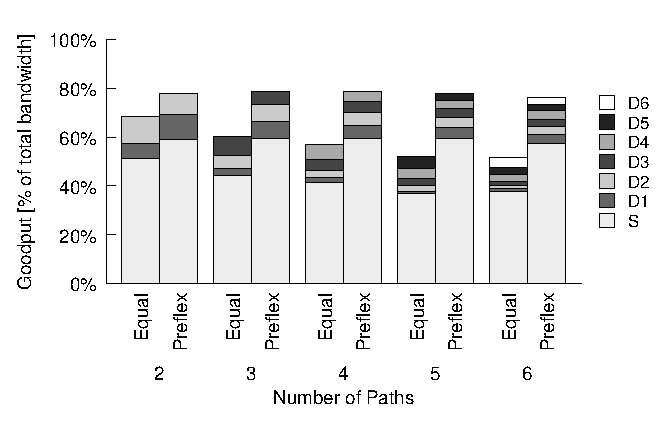
\includegraphics[width=4in]{figures/cate/diffbw}
    \caption{Goodput relative to $B$ achieved by each server for different capacity links.}
    \label{fig:goodputdiff}
\end{figure}

Where bottleneck bandwidth is unequal however equalisation proves inadequate. 
Once again comparing goodput (figure \ref{fig:goodputdiff}) we highlight two significant shortcomings of equalisation which \ac{PREFLEX} overcomes. 
Firstly, goodput for $S$ drops as $N$ increases. 
Unable to realize it is overloading a path, equalisation is reduced to sending traffic over each link at approximately the same rate as the most congested link. 
In contrast, \ac{PREFLEX} detects congestion and adapts accordingly. 
Secondly, the incorrect distribution of traffic due to equalisation in $S$ distorts the goodput of others servers. 
While in \ac{PREFLEX} goodput from $D_{1-N}$ is perfectly balanced, with equalisation traffic crossing the most congested links are directly affected by another domain's inability to distribute its traffic appropriately.
It may seem unfair to judge equalisation for cases where there is a mismatch in link capacity, however this mismatch between link weight and path capacity arises regularly as operators continue to adjust traffic engineering according to local conditions, with little thought spared for the impact this may have further downstream.

\begin{figure}
    \centering
    \includegraphics[width=3.2in]{figures/cate/duration}
    \caption{Mean average flow completion time for equal and differing bottleneck links.}
    \label{fig:duration}
\end{figure}

This impact is in turn perceived by users, who experience longer flow completion times, as shown in figure \ref{fig:duration}. 
In the equal bandwidth case the flow completion time is similar for both balancers.  
Where bandwidth differs however, \ac{PREFLEX} outperforms equalisation and maintains a stable performance when balancing over all six paths.  
This shows that the algorithm scales well as the number of available paths increases. 


\section{Conclusions}
\label{section:malawi:conclusion}

The focus of this work has been on elucidating the main factors that affect flow throughput, but which escape traditional TCP modelling based on end-to-end loss and delay. 
In particular, we explore the changing role of \emph{host limiting}, \emph{application pacing} and \emph{receiver shaping} in defining flow rates across five years of transit traces.
Our results show that for the observed link, over \emph{half} of all inbound TCP traffic can be ascribed to one of the aforementioned constraints.
We show that continuing OS upgrades have progressively lifted the artificial throughput constraints imposed by the host stack. In particular, windowscale negotiation for inbound traffic increased threefold in the observed period, covering over 80\% of all observed bytes by 2012; in addition, we show that buffer sizes have also shown continuing increases over time.

These developments have significantly improved throughput, in particular for smaller flows. However, we also found evidence of throughput limiting effects independent from available end-to-end capacity. This means that no amount of bandwidth will directly improve TCP rates for a considerable amount of traffic.
We show that application-driven techniques for chunked transfer are widely used, accounting for 40\% of all inbound traffic observed in 2011.
%, and that this behaviour is endemic to a wider range of stakeholders than in 2007.
Finally, we uncover evidence of significant receiver traffic shaping prior to 2011 based on the modification of the receiver advertised window in a bid to curtail congestion.
%Uncover evidence of receiver shaping during period of relative contention.



\chapter{A longitudinal analysis of \acs{TCP} traffic}
\label{chapter:malawi}

\renewcommand{\locfolder}{\chapfolder/malawi}
\section{Introduction}

% generic "failures are bad"
Despite being broadly designed for robustness, the current Internet architecture remains remarkably vulnerable to failures.
Managing faults effectively poses a significant operational challenge, in part because faults differ widely in both source and nature, potentially occuring at any layer of the stack and along any element along a path.

% neither is transport
\LOREM
\LOREM

% network methods
Given the commercial nature of the Internet, the onus of providing resilience has instead shifted to network operators.
Traditionally this has been achieved by overloading the routing architecture.
The deployment of real time applications with harder constraints on reliability coupled with better failure detection methods embedded in linecards have provided both the motivation and the means for achieving sub-second recovery within IGP networks \cite{}.
Even with reduced recovery times however, the transient effects of routing changes can still disrupt the forwarding path. 
Under such cases diverse proposals such as Fast Re-Route \cite{}, Loop-Free Alternate next hops \cite{} or Packet Re-cycling \cite{} can provide repair paths for use between the detection of a failure and the convergence of the routing process.

Unfortunately, such methods are rarely sufficient.
Firstly, their application is circumscribed to individual domains, and as such cannot provide end-to-end coverage in a federated, best-effort Internet.
Secondly, there are many faults which do not directly pertain to routing, such as middlebox misconfiguration or hardware malfunctions, and as such go undetected.
Finally, reparation often disregards and potentially disrupts the transport layer by causing out-of-order delivery of packets.

% why now. datacenter, SDN
\LOREM
\LOREM
\LOREM

% layout?
\LOREM
\LOREM


%Outside their networks however, operators are reduced to negotiating service level agreements with their own providers who are invariably unable to cater for such specialized demands \cite{}.
%Even if such terms were met, the Internet architecture provides limited visibility beyond one's own domain.
%This opaqueness, in addition to the fact that failures themselves may be distributed in nature \cite{}, severely limits the ability for a customer network to trace remote problems to a single source \cite{}.
%With no means to hold providers accountable for failures, there is little to enforce the terms of a truly end-to-end SLA.
%
%Unfortunately, such intradomain methods 


%Alongside this increased centralization of resources comes a heightened sense of accountability.
%The commercial nature of the agreements between customers and cloud hosting companies such as AWS \cite{} often involve the establishment of service level agreements.
%Even where such agreements are not explicit, such as the base option of tiered services such as Dropbox or Heroku, there is an inherent need to minimize the impact of outages -- non paying customers may be less demanding, but they are also less sensitive to the switching cost incurred in changing service provider.
%
%Unfortunately, the federated, best-effort nature of the Internet seemingly does not lend itself to such high expectations.



%Under such cases, a network operator is currently expected to detect, repair and recover from such faults.
%Detection often requires scale -- the reliability with which a fault can be identified relies on the proportion of traffic affected. 
%In many cases, faults affecting single flows may go undetected by the network.
%Once detected, reparation varies according to the nature and origin of the fault.
%For some cases, such as intradomain routing, this process is often automated and robust.
%For many others however, such as faulty hardware or misconfigured devices, recovery is difficult and error-prone.
%In either case, the amount of time expended in detection and repair can often preclude recovery, since most flows will terminate after successive timeouts.
%

%Fueled largely by economies of scale in both software management and hardware acquisition and maintenance, the emergence of cloud computing and content distribution networks has lead to a profound shift in Internet traffic.
%
%
%Whereas the advent of broadband connections init
%In contrast to the highly distributed nature of peer-to-peer software which 
%
%
%For one, never has so much been distributed by so few to so many.
%% AS dist graph
%% netflix
%
%\LOREM
%
%% Accountability, resilience

%All intervening equipment is subject to failure along a network path, with recovery time depending not only on \emph{what} happened, but also \emph{where}.
%Within their networks, operators are free to instrument and deploy arbitrarily complex tools to meet requirements. 
%This freedom has lead to a proliferation of proposed improvements in resilience for intradomain settings \cite{}.


%The establishment of SLAs for network availability have traditionally been prefered within the telecom industry in particular, and represent one possible approach to ensuring resilience. An alternative approach is offered by the end-to-end principle. 
%Since end hosts possess both inherent knowledge of application needs and fine-grained measurements on end-to-end path characteristics, the transport layer is often identified as a more natural fit for dealing with fault tolerance at an Internet scale.
%Both SCTP \cite{} and MPTCP \cite{} enable transparent fail-over through multihoming.
%In spite of providing significant features, neither is likely to be widely deployed in the near future: the former lacks critical middlebox support, while the latter is still undergoing standardization.
%Furthermore, the requirement for end-host multihoming has also posed a barrier to deployment.
%Finally, all transport approaches to fail-over confine knowledge of faults within an individual flow: each flow must detect failures independently, even when many flows are affected by the same fault.
%


% Transport is not the answer

% Can we do better with SDN?


%A default forwarding plane, corresponding to the label 0, must be defined and cater for all traffic destinations.
%As with existing routing infrastructure, this single default plane will suffice for most traffic.

%Invariably however, path failures will arise which may affect any number of flows.
%Rather than expecting the network to address end-to-end failures, hosts are allowed to proactively request an overlay plane from the network.





\section{Related work}
\label{section:malawi:related}

Despite their inherent value, longitudinal studies of Internet phenomena are rare. 
Over its short lifespan the Internet has been shaped as much by technological change as by political and commercial realities. 
This dynamic nature does not lend itself to observational studies where data must be collected and curated over long periods of time, and has resulted in a scarcity of relevant datasets. 
What few exceptions exist often stem from collaborative research efforts, such as CAIDA \cite{CAIDA} or Oregon Routeviews \cite{routeviews}. 
The usefulness of these datasets however can be severely affected by the need for data privacy. 
The dissemination of interdomain routing information, where no such requirement exists, has assisted in a wealth of research on wide ranging topics, from quantifying path diversity \cite{Oliveira:2009p203} to locating Internet bottlenecks \cite{Hu:2004p96}. 
In contrast, longitudinal datasets relating to passive measurements have nurtured a much smaller community of researchers often focusing on characterizing traffic \cite{Fontugne:2010p413}. 
Stripped of the locality contained within IP addresses however, researchers are left unable to relate these findings to a wider context.
Instead, cross-sectional studies characterizing traffic aggregated by location are frequently conducted under different contexts \cite{Ager:2011:WCC:2068816.2068870}, but lack the temporal perspective only longitudinal studies can afford. 
Efforts to characterize the spatial properties of traffic over time \cite{Dhamdhere:2011p428,Labovitz:2010:IIT:2043164.1851194,Cho:2008:OSC:1544012.1544024} have defined the changing of Internet topology and traffic alike but fall short of relating such shifts with their impact on relevant metrics such as loss or delay. 

% other work since
This chapter builds on a wealth of prior work on understanding Internet traffic and serves as a reappraisal of significant past contributions.
Flow characteristics and \ac{TCP} behaviour at large are subject to frequent reassessment \cite{Zhang:2002p85}.
Of particular relevance to the current work are passive studies which delve into the inner mechanisms of \ac{TCP}.
In \cite{Jaiswal:2004p242}, Jaiswal et al.\ infer the sender's congestion window by identifying the congestion control variant from the behaviour observed during loss recovery.
The use of separate state machines for each variant however proves unscalable given the many flavours of \ac{TCP} congestion control which have since been deployed.
In \cite{Lan:2006p566}, Lan et al.\ analyse flows according to size, duration, rate and burstiness and characterise the observed correlations for heavy-hitters specifically,
uncovering evidence of increased application influence on flow rates and burstiness and consequently suggest treating flow size and duration as independent dimensions.

One central aspect to the analysis of \ac{TCP} behaviour is the estimation of \ac{RTT} from packet capture data. 
In addition to SYN-based methods, Shakkotai et al.\ \cite{Shakkottai:2004p408} evaluate further techniques to estimate the \ac{RTT} of a unidirectional flow. 
The \textit{rate change} method establishes a relation between the \ac{RTT} and the increase in sending rate, assuming linear window increases during congestion avoidance. 
Unfortunately, this assumption no longer holds, both due to the proliferation of less conservative congestion control algorithms such as CUBIC \cite{Ha:2008p471}, and due to application-driven flow control. 
An alternative is the use of frequency-domain techniques \cite{Veal:2005p412,Lance:2005p565,Qian:2009p429}, which are a natural fit given the self-clocking nature of \ac{TCP}. 
However, a common difficulty with the application of spectral analysis is extracting the fundamental frequency which corresponds to the \ac{RTT} in the presence of noise. 
In applying the Fourier transform to inter-packet arrival times, for example, Qian et al.\ \cite{Qian:2009p429} note that less than half of all flows have distinguishable \textit{flow clocks}; likewise, the \ac{FFT}-based \ac{RTT} recovery was found to be unreliable even after pre-processing available data to enhance inherent periodicities.

% topological influence
Finally, it is important to elucidate what changes in traffic properties are intrinsic to \ac{TCP} and data transfer, and which ones arise from large-scale changes in the \ac{AS}-level topology of the Internet. 
In the decade since publication of \cite{Zhang:2002p85}, the Internet has undergone significant changes, shifting from a broadly hierarchical form to a flatter, more interconnected structure \cite{Labovitz:2010p175,Ager:2012p567}.
Given the longitudinal nature of this chapter and its focus on interdomain traffic in particular, the insights provided by these studies on the macroscopic effects of content consolidation are discernible within the studied dataset, and as such are a source of validation for many of the observations herein.

\section{Dataset}
\label{section:malawi:dataset}

This section provides an overview of the datasets used in this work and some of the data processing required before approaching the longitudinal study of Internet traffic rate limiting. We use the original, unanonymised traffic traces of the MAWI \cite{mawi} dataset, a set of daily traces from the WIDE backbone network which provides connectivity to universities and research institutes in Japan. Traffic is captured daily for 15 minutes starting at 14:00JST. Although this dataset extends back largely uninterrupted from late 2001, we focus on just over five years of data following a network upgrade to the monitored link on October 2006.

The monitored link carries mostly trans-Pacific commodity traffic between WIDE customers and non-Japanese commercial networks. 
We will refer to traffic towards WIDE as \emph{inbound} traffic, whereas traffic originating from within WIDE is referred to as \emph{outbound} traffic.

\begin{table}[!htp]
\scriptsize
\centering
    \begin{tabular}{r|cccccc}
        & & TCP data & \multicolumn{2}{c}{Traffic (TB)} & \multicolumn{2}{c} {Count ($\times10^3$)} \\
        Year & Days & flows (x$10^6$) & In & Out & AS & Prefixes \\
        \hline
        2006 & 91 & 20.52 & 0.43& 0.45 & 10.90 & 56.86\\
        2007 & 350 & 102.56 & 2.11 & 2.49& 17.21 & 113.79\\
        2008 & 358 & 112.26& 2.43 & 2.10& 24.74 & 156.54\\
        2009 & 364 & 113.97& 2.48 & 2.53& 19.71 & 143.87\\
        2010 & 365 & 113.70& 2.58 & 3.43& 20.38 & 148.03\\
        2011 & 358 & 114.74& 3.44 & 5.14& 19.99 & 140.56\\
        \hline
        Total & 1886 & 5777.55 & 13.50 & 16.14 & 34.12 & 341.22\\
    \end{tabular}
    \caption{\label{table:overview}Overview of traced MAWI dataset 
}
  \vspace{-3mm}
\end{table}

A preliminary overview of the dataset used is provided in table \ref{table:overview}. 
In total, 5.7 billion flows containing data are traced over five largely uninterrupted years; this represents approximately 30 terabytes of TCP traffic. For the purposes of this work, we will focus exclusively on inbound traffic, 60\% to 80\% of which originates from port 80, referring only to analysis of outbound traffic when providing a wider context for our findings.
Given the sender side plays a critical role in shaping traffic, analysing traffic for which the source is restricted to a small set of networks within Japan would be of limited use in accurately depicting traffic trends at large.
We instead fix hosts within Japan as sinks, thus sharing a similar perspective on inbound traffic as many other networks. 

\subsection{Tracing TCP Metrics}

All TCP flows are reassembled and analysed for each daily trace.
In addition to the five tuple used to define each connection, we impose two additional restrictions: a contiguous sequence number space and a three minute timeout. These restrictions are helpful to deal with port reuse and unterminated flows respectively.  
Although the total number of TCP flows increased dramatically in 2011, the number of flows \emph{for which data payload was seen} has remained stable, averaging over 100 million data flows traced per year.  

There is much prior work with regards to reconstructing TCP flow from passive measurements and using this information to understand the end-to-end properties of traffic \cite{firstRTT,Jaiswal:2007p233,Rewaskar:2007p195,Shakkottai:2004p408}. However, the MAWI traces impose two constraints which require careful consideration, and ultimately led to the use of a custom TCP tracer. 
The first one is the proportion of bidirectional flows, that is flows, where both forward and reverse path are seen. 
In the dataset used this fluctuates between 40\% and 60\% over five years.
Most available TCP tracers either ignore or are inadequate at processing unidirectional flows. 
The second one is the short duration of each individual trace file. 
At only 15 minutes of line-rate data capture per day, it is wasteful to ignore flows which are not complete. Although the number of flows for which a SYN and FIN in either direction is observed has remained consistently high until late 2011, these flows are normally \emph{mice}, i.e. flows that tend to be brief and which carry little traffic individually. In contrast, most \emph{elephants} (flows that carry significant traffic individually) have durations that exceed that of each trace file. 

%rtts traced
%While many metrics are extracted for each flow, for the purposes of this paper we will focus only on detailing how we collected delay and loss.
%Passive RTT estimates, calculated as the offset between a data packet and its respective acknowledgement, require both directions to be observed at the measurement point. 
%This provides delay estimates between the measurement point and the receiver, as illustrated in figure \ref{fig:synrtts}. 
%For flows where data is transfered in both directions, we will obtain in effect two separate estimates, $RTT_{m2a}$ and $RTT_{m2b}$, illustrated in figure \ref{fig:synrtts}. 
%Together they form the total end-to-end delay experienced by end-hosts. 
%For the remainder of this paper, the term RTT will refer to delay between our measurement and destinations outside WIDE. 
%We discard the delay between measurement point and hosts within WIDE for two reasons. 
%It is both negligible for a large proportion of traffic, which is highly concentrated within the Tokyo metropolitan regions and immediate surroundings, and extremely large for a very small subset of hosts located outside Japan, as WIDE has in the past acted as a provider to academic institutions in Indonesia through a satelite uplink. 
%By decoupling both directions we focus purely on the changes in delay to locations outside Japan. 
%This incurs a reduction in the range of destinations for which we can obtain estimates - only bidirectional traffic can be traced this way. 
%For the set of destinations we will study in this paper, we shall show that this reduction is small. 
%For tracking delay changes for unidirectional traffic for other purposes, MALAWI includes RTT estimates extracted from the SYN exchange.

Loss is inferred by accounting for \emph{retransmissions} in the upstream data and \emph{out-of-order packets} in downstream data; for the remainder of the paper we will refer to the \emph{end-to-end loss} as the sum of out of order and retransmitted data bytes over the total data bytes in a given direction.
% XXX: remove RTT ref?
%Tracking both retransmissions and out-of-order packets accurately requires a reliable RTT estimate, which can only be obtained for bidirectional flows. We forfeit some precision by not taking this into account, as we wish to be consistent in how we estimate both metrics independently of the type of flow and aggregation. 
Pragmatically, we found this to be an adequate indicator of loss --- with the exception of \emph{hanging} TCP connections. 
In these cases where connectivity is lost, a host will proceed to retransmit packets while performing an exponential backoff. 
Although this results in negligible overall traffic, it can significantly skew the inferred loss ratio for uncommon destinations for which little traffic exists. 
To account for these cases, we imposed a 3-second timeout on retransmissions after which we consider the congestion feedback loop to be broken. 

Each daily trace in the dataset is processed from a packet level capture into a collection of flow level statistics. 
This gives us insight into the end-to-end characteristics of traffic. However, since a core objective of this work is to augment this time-based information with data describing the endpoints of each flow, aggregating by location is also required. 

\subsection{Aggregating by Location}

Location information is added by mapping the original source and destination IP addresses to its geographical and topological counterpoints. 
We use the \emph{routeviews} archives to reconstruct the mapping between each IP and both AS and network prefix; bi-hourly dumps of BGP RIBs are available in the WIDE archives since mid 2003. 
We reconstruct a daily RIB based on the views provided by contributing ASes, in particular IIJ and APNIC. 
Since exact routes are not disclosed (there is no record of local policy), we have no knowledge of the route taken by packets; this of course does not hinder our ability to consistently map IPs to ASes. While discrepancies in AS destinations exist between different routeviews contributors, we note that this happens almost exclusively on prefixes for which no actual traffic is seen. 

Mapping IP to country is done through the use of GeoLite \cite{maxmind}, a commercial geolocation database. 
While the accuracy of this solution is often disputed, we are not overly concerned with locating traffic at a fine granularity. 
We will mostly focus on tracking traffic by country and, for larger countries such as the U.S, by region, in order to capture shifts over time.
GeoLite proves adequate on both counts.
The archive for geolocation data only extends to 2009, before which we must rely on the earliest match. 
Additionally, we verify if the destination or source AS have maintained the same administrative mapping up until mid 2009 in the relevant RIR (regional internet registry) archives; otherwise, we do not associate a flow to a geographical location.
% bridging paragraphs to save space.
After associating flows to country, region, AS and network prefix for both source and destination IPs, we aggregate flow statistics over each location identifier. 
This generates a daily collection of location identifiers and associated flow properties, from which we can sketch the geographic and topological properties of the dataset over time.

\section{Methodology}

Providing a macroscopic view on where traffic originates from, and in what quantity, can be achieved by simply binning packets into flows and accumulating byte counts over geographical or topological locations. 
Uncovering application layer characteristics (i.e. \textit{how} traffic is sent) is a more complex problem that requires additional methods to reverse engineer transport behaviour.
The aim of this section is to describe a process which distinguishes those flows which have their throughput limited by mechanisms other than the usual \ac{TCP} response to loss and delay.
Each flow can be characterized as being either application paced, in which the sending application is limiting the data provided, host limited, whereby local constraints at either end host cap throughput, or receiver shaped, in which an artificial constraint is imposed by either a middlebox or receiver.

The classification proceeds in stages. 
Before classification, it is necessary to reconstruct the RTT of the flow if the flow is not bidirectional.  
This is achieved in section \ref{subsection:malawi:PeriodicEnhancement}. 
Because the sender's TCP state machine cannot be directly observed it is necessary then to estimate the size of the congestion window by observing the number of unacknowledged bytes in flight (\textit{flight size}).
This reconstruction is described in section \ref{subsection:malawi:flightAggregation} and provides the basis for flow classification. 
Flows are then checked in turn to see if they are application paced, host limited or receiver shaped and classified as belonging to the first of these classes for which they fulfill the necessary conditions.
Flows in none of these classes are either limited only by the network (delay or loss conditions) or are insufficiently large to trigger any further constraints.

\subsection{RTT Estimation}
\label{subsection:malawi:PeriodicEnhancement}

Building on prior work presented in section \ref{section:malawi:related}, this section proposes an algorithm that scalably recovers the RTT from one-directional traffic traces. 
% XXX: below implies microflights were used, but these aren't described (remove as appropriate)
Although \ac{RTT} estimation is a difficult problem, simplifying assumptions can be made.
For the \ac{MAWI} dataset most \acp{RTT} are relatively large, with the closest neighbouring country, South Korea, roughly 40ms away.
By only processing bidirectional traffic from Japan, the expected \ac{RTT} range can be reduced for all other traffic.
The recovery mechanism then enhances the natural periodicity of traces and scalably constructs flights associated with specific application and protocol behaviour.
In the following the mechanisms required by these two goals are described. 
%
% Why does this work?
%
In normal operation, many \ac{TCP} operations involve request-response cycles between two endpoints in which the \ac{RTT} $T$ provides a natural \emph{clock}.
Hence, the most natural way to estimate \ac{RTT} from \ac{TCP} traces is to correlate requests and responses exchanged in both directions. 
If only one direction of data is observed however, $T$ cannot be directly observed. 
Instead, it must be estimated from the way in which \ac{TCP} packets cluster in time due to the batching of request-response operations.

The \ac{TCP} \ac{cwnd} determines the number of unacknowledged bytes that a \ac{TCP} flow may maintain at any point in time. 
This can be referred to as \emph{bytes in flight} because they are in transit between the sender $S$ and the receiver $R$; an equivalent definition applies for the number of \emph{packets in flight}. 
Once $S$ has transmitted \ac{cwnd} data bytes, it will refrain from transmitting more until either some bytes are acknowledged by $R$ or \ac{cwnd} is increased by the sender. 
In the absence of losses, neither of these events can happen until a \ac{TCP} \ac{ACK} is received; this immediately reduces the number of unacknowledged bytes, but may also lead to a significant \ac{cwnd} increase (during e.g. \emph{slow start}). 
% XXX: number of unacknowledged bytes reduced, or CWND?
In the presence of losses, however, bytes can be re-sent if a packet is timed out and considered lost; in this case, the number of unacknowledged bytes is reduced.

%
% What is our main contribution, algorithmically speaking?
%
The main difficulty associated with one-sided TCP flow reconstruction is as follows.
Let $t_1, t_2, \ldots$ be a set of times at which packets $p_1, p_2, \ldots$ were observed at $S$ en route to $R$.
Suppose that a packet $p_j$ of size $b$ is observed at time $t_j$.
In addition, suppose that approximately one RTT $T$ later, the sender $S$ receives an ACK $a_j$ from $R$ for the $b$ bytes of $p_j$.
At this point, the TCP stack in $S$ will decrease the number of unacknowledged bytes by $b$, thus opening the possibility for sending additional traffic to $R$.
This can lead to another packet $p_k$ to be transmitted; let this packet be observed at time $t_k$ as it is sent towards $R$.
Assuming that processing delay is insignificant, the RTT experienced by $p_j$ can be approximated as $T \approx t_k - t_j$.
Now consider what happens if packets are only observed in the $S \rightarrow R$ direction.
Under such conditions, it is not possible to ascertain whether $p_k$ was sent explicitly as a result of $S$ receiving the unobserved \ac{ACK} $a_j$, or whether it was sent as a result of an \ac{ACK} $a_i$ associated with a previous packet $p_i$ rather than with $p_j$.
If, however, a packet $p_l$ is eventually observed that did result from the reception of $a_j$, the \ac{RTT} can be estimated as $T \approx t_l - t_j$ with $t_l > t_k$.
Following this same reasoning, approximately one \ac{RTT} later a packet $p_m$ will be observed for which $2T \approx t_m - t_j$; this can potentially continue for as long $S$ has data to send and $R$ continues sending \acp{ACK}.
This is the underlying reason that \ac{RTT}-related periodic regularities arise when considering the timestamps of observed packets \cite{Qian:2009p429}.

The reasoning above is at the heart of the proposed algorithm to improve \ac{RTT} recovery by enhancing packet stream periodicity. 
Assume that a packet $p_j$ is observed at time $t_j$. 
Considering the set $\mathcal{T}_j$ of all values of $\Delta t = t_k - t_j$ for every $k > j$, it is apparent that it will include estimates not only for the \ac{RTT} $T$, but also for all its multiples $2T, 3T, \ldots$ 
If $t_l-t_k \approx T$ and $t_k - t_j \approx T$ then it follows that $t_l - t_j = 2T$, and this value will also be included in $\mathcal{T}_j$. 

By maintaining a set $\mathcal{T}_j$ for every packet $p_j$ observed, at least some of its values will correspond to estimations of multiples of the \ac{RTT}. 
It then follows that by creating a set $\mathcal{T}$ that includes values calculated starting from every packet $p_j$ so that $\mathcal{T} = \cup_j \mathcal{T}_j$, numerous estimates for $2T, 3T, \ldots$ will also be included. 
Hence, the probability density function $H(t)$ of the values in $\mathcal{T}$ should show peaks around multiples of the \ac{RTT} (see Figure \ref{fig:histogram}). 

\begin{figure}
  \centering
  \includegraphics[width=0.8\textwidth]{figures/malawi/rttbin.pdf}
  \caption{$H(t)$ for flow displayed in Figure \ref{fig:hostlimited}. The horizontal line delimits $\overline{H}$ while the highlighted bin denotes the bidirectional RTT estimate.\label{fig:histogram}}
\end{figure}

%
% Explain why did we use FFT
%
The algorithmic recovery of $T$ from $H(t)$ presents additional challenges. 
In particular, $H(t)$ may include a large number of \ac{RTT} multiples, and a peak will be found for all of them. 
Crucially, all these peaks may be of comparable magnitude, complicating the task of selecting a single peak.
Moreover, these peaks need not be very pronounced, with histogram bins in close proximity of the peaks have very similar values as the peak itself. 
As such, taking \ac{RTT} candidates directly from $H(t)$ may result in a large set of similarly-valued bins situated around a peaks at multiples of the \ac{RTT}. 

Three recovery algorithms for $T$ are attempted.
First, as a baseline, the highest peak in $H(t)$ is selected as a candidate for $T$. 
In addition, expanding upon the work of Qian et. al. \cite{Qian:2009p429} a frequency-domain representation of $H(t)$ is used to identify $T$. 
This is done by selecting the highest peak of $|\hat{H}(\omega)|^2$, the \emph{energy spectral density} of $H(t)$ (i.e. the norm squared of the Fourier transform of $H(t)$). 
Finally, a custom utility-based technique that operates directly on $H(t)$ is proposed which achieves superior performance to both of the aforementioned methods.

%\subsubsection{FFT-Based RTT Recovery}
%We extract periodicity information from $H(t)$ by looking at $\hat{H}(\omega)$, the \emph{energy spectral density} of $H(t)$. Formally, $\hat{H}(\omega)$ is defined as the norm squared of the Fourier transform of $H(t)$, so that $\hat{H}(\omega) = |\mathcal{F}(H(t))|^2$. Using $\hat{H}(\omega)$ markedly improves the quality of our RTT estimation because the frequency peak corresponding to the RTT usually accounts for a much larger proportion of the total frequency domain energy than other peaks in $\hat{H}(\omega)$, leading to a much simpler discrimination of the true RTT. However, due to RTT changing during the lifetime of a flow, and also due to the expected noise associated with real-life data sources, $\hat{H}(\omega)$ can also occasionally include large peaks at frequencies unrelated to the RTT. In order to filter these out, we take a set of 10 frequency candidates from $\hat{H}(\omega)$, and use their associated periods as RTT candidates in our flow reconstruction algorithm (see Section \ref{
%subsection:malawi:flightAggregation}). We then select that RTT candidate which exhibits the smallest error, that is, that one which yields closest agreement with observed data.

%
% Algorithmic hacks
%
%To streamline our algorithm for streaming use, we use the following heuristics and approximations. Firstly, we define a range $[T_{\min}, T_{\max}]$ representing the range over which we find the RTT values of interest. Then, for each packet $p_j$, we build a subset $\mathcal{T}_j'$ of $\mathcal{T}_j$ by including all values of $t_j - t_k < T_{\max}$. We then generate $\mathcal{T}' = \cup_j \mathcal{T}_j'$ and approximate $H(t)$ by considering a histogram of the values in $\mathcal{T}'$. As usual, we do this by counting the frequency with which its values are observed in the ranges $[0,\tau)$, $[\tau, 2\tau)$, $[2\tau, 3\tau), \ldots$ where $\tau$ is the time resolution required. 


\subsubsection{Utility-Based RTT Recovery}
\label{sect:utilityBasedRecovery}

This method relies not on the identification of periodicities, but on explicitly matching experimentally found signatures. 
To this end, we consider the peaks of $H(t)$, which are then considered RTT candidates.  
However, trivial discriminators (such as simply selecting the highest peak) are not reliable. 
In this case, it was found experimentally that repeatable peaks and troughs also occur at multiples and sub-multiples of $T$, with the most important ones being $\frac{T}{3}$, $\frac{T}{2}$, $T$ and $2T$. 
We design this detection algorithm around the idea that a given pattern of peaks and troughs can identify $T$.

If we define $\overline{H}$ as the mean height of $H(t)$, we can define a per-peak utility function $p(t)$ so that 
\begin{equation*}
p(t) = 1.0 - \exp\left(-2.0 \left(\frac{H(t)}{\overline{H}}\right)\right) \mbox{.}
\end{equation*}
This function has several advantageous properties: it is 0 if $H(t)$ is zero, 1
if $H(t)$ is infinite, and $0.5$ if $H(t) = \overline{H}$.  In other
words it is a measure of the \emph{peakiness} of the data, with $p=1$ identifying
an infinitely high peak, $p=0$ identifying an empty histogram bin (trough), and $p=\frac{1}{2}$ 
implying that $H(t)$ is of exactly average height at that point. We can then score each candidate using the following utility function:
$$
P(t) = 1.5 p(t) + p(2t) - p\left(\frac{t}{2}\right) - p\left(\frac{t}{3}\right).
$$
That is, the candidate RTT $t$ scores highly if it is itself a peak, if it has a peak
at a multiple $2t$, and if it also manifests troughs at submultiples $\frac{T}{2}$ and $\frac{T}{3}$.
The factor of 1.5 was added after observations
showed that the peak at $T$ was the most important factor in determining
whether a candidate was the true RTT. Similarly, additional multiples and submultiples 
were excluded as they showed very limited discriminating power experimentally.

\begin{figure}
  \centering
  \includegraphics[width=0.8\textwidth]{figures/malawi/rttcomp.pdf}
  \caption{Accuracy of RTT estimator when compared to the median value of bidirectional estimate.}
\end{figure}

\subsubsection{Comparing RTT Recovery Algorithms}
\label{sect:comparingRecoveryAlgos}
As described in Section \ref{subsection:malawi:PeriodicEnhancement}, $H(t)$ is calculated in such a way that RTT periodicity is amplified. 
This means that FFT-based techniques could potentially perform better on $H(t)$ than on the packet stream with no pre-processing. 
However, this is complicated not only because $H(t)$ contains periodicities at multiples of $T$, but also discontinuities that generate harmonics at frequency multiples of the RTT fundamental. 
Hence, although the FFT $|\hat{H}(\omega)|$ of $H(t)$ is much cleaner than that of the packet interarrival time series on its own, its maximum peak rarely coincides exactly with the RTT clock (this corroborates reports by Qian et al \cite{Qian:2009p429}). 
Thus, applying the FFT leads to another \emph{peak detection problem} in which the RTT fundamental needs to be extricated from its harmonics and sub-harmonics. 
The trivial solution to this problem, the application of a bandpass filter around the RTT frequency, is of course unfeasible because the bandwidth and 
centring of such a filter depend on the RTT which is itself unknown.
The utility-based algorithm described in Section \ref{sect:utilityBasedRecovery} can hence be applied in either the time domain or the frequency domain; we chose to do it on the former on the interest of expediency and lower computational cost.

\newcommand{\RTTHeader}{Below & Above}
\newcommand{\SmallFlowName}{\textless 10MB}
\newcommand{\LargeFlowName}{\textgreater 10MB} 
\begin{table}
\footnotesize
\centering
\begin{tabular}{ p{1.5cm} p{1.2cm} p{0cm} p{.6cm}p{.6cm} p{0cm} p{.6cm}p{.6cm}}
& & & \multicolumn{2}{c}{Peak} & & \multicolumn{2}{c}{Utility-based} \\
\cline{4-5} \cline{7-8}
& Flow size & & \RTTHeader & & \RTTHeader \\
\cline{4-5} \cline{7-8} 
\multirow{2}{*}{Receiver side}  & \SmallFlowName && 4.31 & 9.13 && 4.58 & 6.35
\\ 
                                & \LargeFlowName && 6.72 & 6.43 & 4.97 & 5.33
\\
\multirow{2}{*}{Sender side}    & \SmallFlowName && 2.94 & 8.37 && 3.29 & 4.80
\\
                                & \LargeFlowName && 6.41 & 9.06 && 5.40 & 11.06
\\
\end{tabular}
\caption{\label{table:rttRecovery}Performance of RTT recovery algorithms}
\vspace{-3mm}
\end{table}

The performance of the analysed RTT recovery mechanisms is presented in Table \ref{table:rttRecovery}, that shows the percentage of total flows below and above the RTT range given by the bidirectional estimates.
We separate things for \emph{inbound} traffic (where we are positioned at the receiver side) and \emph{outbound} traffic (where we are positioned at the sender side). The utility-based algorithm is particularly useful to address RTT underestimation for flows over 10MB in size, which is our main objective since precisely that kind of estimation error would interfere with our ability to correctly decouple application behaviour from RTT-scale dynamics.


%For the most part, the utility based method improves on underestimation, which is our main objective since that would interfere with our flight reconstruction (i.e. generate lots of gaps).
%The exception (kind of) is traffic from the sender side, which in our training set (one week per year), had quite a lot of host limited traffic (paced out, no signal to recover).
%In this case, not a problem, since if the flow is long enough multiples of the RTT will still reveal host limitation, but will give us a smaller window..


\subsection{Flow Classification}
\label{subsection:malawi:flightAggregation}

One fundamental precondition to decouple the influence that network loss, host configuration and TCP behaviour has on the throughput experienced by a flow is the reconstruction of the congestion window behaviour of TCP flows on the basis of observed data. 
Unfortunately, the congestion window value is internal to the sender's TCP state machine and may not manifest itself in the absence of sufficient data from the application layer. 
A more easily observed quantity which serves as a reasonable proxy for the congestion window is the number of unacknowledged bytes in flight, henceforth referred to as the \textit{flight size}, which can be derived given an accurate estimate of the end-to-end delay.
The evolution of both flight size and RTT can in turn be used to ascertain to what extent throughput is regulated by limitations imposed at different layers of the networking stack.

% definitions
Given a candidate RTT, we can aggregate a stream of packets with arrival times $t_1, t_2, \ldots$ into a stream of \emph{flights}. 
Intuitively, a flight is a clustered subset of a TCP flow which exhibits its own temporal coherence; alternatively, it can be though of as a series of consecutive packets that were (roughly) generated by the sender as a response to the same protocol operation. 
A flight $f_i$ that begins
with the $j$th packet and ends with the $k$th is defined to have a \emph{total flight time} $\tau_i = t_{k+1} - t_j$. 
The algorithmic selection of initial and final packets in such a way that the resulting flights are indicative of TCP behaviour remains an open problem. 
Since we assume that the RTT provides a natural time frame for the operations of TCP, in the algorithm presented in this work, given an initial packet $\pi_j$ and an RTT estimate $T$, the $k$th (and final) packet is selected to minimise \emph{the flight time error} $e_i = |T - \tau_i|$. 
This mechanism follows closely the methodology described in \cite{Zhang:2002p85}, with the exception that we do not attempt to define flights as being both adjacent and disjoint; rather, we decompose flows into a stream of potentially overlapping flights. 
This helps the algorithm mitigate the deleterious effects of small deviations in the estimated RTT, which alters the properties of each flight. 
Furthermore, since the flight size is continuous in time, it makes little sense to restrict ourselves to a single sample per round trip time.

Having obtained flight information from each flow, we next consider what is the predominant factor that affects its throughput. 
Within the context of TCP, we classify flows as being artificially constrained by three distinct processes: \emph{application pacing}, \emph{host limited} and \emph{receiver shaping}.

\begin{figure}
\centering
  \centering
  \begin{subfigure}{1.0\linewidth}
    \includegraphics[width=1.0\textwidth]{figures/malawi/youtube.pdf}
    \caption{Application paced. \label{fig:youtube}}
  \end{subfigure}\\
  \begin{subfigure}{1.0\linewidth}
    \includegraphics[width=1.0\textwidth]{figures/malawi/hostflow.pdf}
    \caption{Partially host limited. \label{fig:hostlimited}}
  \end{subfigure}\\
  \begin{subfigure}{1.0\linewidth}
    \includegraphics[width=1.0\textwidth]{figures/malawi/awnd.pdf}
    \caption{Receiver shaped. \label{fig:awnd}}
  \end{subfigure}
  \caption{Flight size over time for flows affected by different artificial constraints. \label{fig:kindsOfFlowEffect}}
\end{figure}


\subsubsection{Application Paced Flows}
\label{sssec:app}

A flow whose throughput decreases because it has no outstanding data to send is temporarily limited by the application. 
Flights can be identified as being \emph{application limited} if terminated with a packet smaller than the maximum segment size (MSS) and followed by an inter-arrival time greater than the RTT, as consistent with \cite{Zhang:2002p85}. 
The underlying reason for this defintion is that most TCP implementations will wait some time for subsequent bytes to be written to the socket if the next packet to be sent is smaller than the MSS, unless the TCP\_NODELAY option is set \cite{nagle1984rfc}.

A flow with \emph{application limited} flights however is not necessarily \emph{application paced}. In practice, all flows for which the final packet is observed contain at least one such flight.
For the purposes of our work, we are focused on identifying cases in which throughput is predominantly determined by application behaviour.
One such example is illustrated in figure \ref{fig:youtube}, in which a stream is delivered by periodically writing blocks to the sending socket.
The resulting network-level behaviour is distinct from traditional congestion control: short bursts are interspersed with protracted silence.
Application limited flights, which terminate on non-MSS packets, are highlighted at the end of each burst.

This behaviour is in stark contrast to that exhibited in figure \ref{fig:hostlimited}, where distinct transfers are multiplexed on top of a single transport association over time.
From the perspective of the network, there is little to distinguish the behaviour of such traffic from independent TCP flows.
Application paced connections such as Youtube traffic however exhibit a degree of regularity which can potentially be exploited by the network in predicting demand or smoothing bursts.

In order to identify such recurring behaviour, we identify flows as being \emph{application paced} if the period between bursts terminated by \emph{application limited flights} is consistently under 10 seconds and the standard deviation of the intermediate pauses is under one second.
This definition in particular purposely ignores flows which exhibit long silence periods due to user interaction, and follows closely the behaviour historically associated to Youtube streaming in particular.

\subsubsection{Host Limited Flows}
\label{sssec:host}

Given sufficient bandwidth and traffic to send, a flow may encounter local constraints at either end-host which cap its throughput. 
For instance, the buffer space allocated on both the sender and receiver side is often pre-configured, and it is common practice to tune these values down on popular servers and managed infrastructure in a bid to conserve memory or bandwidth.
A receiver is also limited in the window size it can announce to the remote sender; if the windowscale option \cite{jacobson1992tcp} is not negotiated during the TCP handshake, the advertised window cannot exceed 64KB.

In both cases, a local decision by either host can determine the upper bound of the flow rate.
These \emph{host limited} cases are characterised by a constant window size over time.
The methodology described for flight aggregation at the beginning of this section typically generates a large number of flights, representing many likely combinations given a base RTT estimate.
In order to identify the flat-lined behaviour of a host limited flow, we first filter the flight stream to remove some of the uncertainty derived from small fluctuations in the RTT.
We then select the maximum flight size observed for each RTT interval, and declare a sequence of flights to be host limited if the same maximum was observed over six consecutive RTTs (this is twice the period suggested in \cite{Zhang:2002p85}).
In practice, increasing the period over which the maximum window size is tracked allows us to more accurately discern between host limited behaviour and more conservative bandwidth probing, such as that performed during the convex phase of TCP CUBIC \cite{Ha:2008p471}.

A flow may be host limited for only brief periods of its lifetime, as illustrated in figure \ref{fig:hostlimited}.
To filter out such cases where host limitations are not the predominant factor in defining flow throughput, we further enforce that in addition to host-limited flights, the average window size must over a flow lifetime should be within 10\% of the inferred host limit, which is not the case in figure \ref{fig:hostlimited}.

In practice, flows can exhibit both application pacing and host limitations, with bursts being sent at a capped window size followed by application pauses.
In such cases, a flow will still be classified as being \emph{application paced} if it meets the requirements set out in the previous section, as doing so provides evidence that it controls throughput in spite of the degraded performance provided further down the stack. 
This line of reasoning applies equally to the occurrence of sporadic loss; so long as block delivery is ensured within the timeframe dictated by the application, it remains in control.

\subsubsection{Receiver Shaped Flows}
\label{sssec:rec}

A flow which is neither \emph{application paced} or \emph{host limited} can still be artificially constrained by flow control (rather than by congestion control).
Traditionally, in TCP the sender is responsible for regulating throughput. 
However, the receiver can also shape throughput by manipulating the \emph{advertised window} announced on every acknowledgement.
Such receiver-window auto-tuning has been available on Windows operating systems since Vista \cite{vistaReceiveWindow}, and can also be leveraged by middleboxes in order to throttle inbound traffic \cite{appEx}.

In order to evaluate the potential impact of such behaviour, we further propose a heuristic to identify receiver-shaped traffic.
For flows in which both directions of traffic are observed it is possible to correlate the evolution of the advertised window with the size of reconstructed flights.
Figure \ref{fig:awnd} displays an example of a receiver-shaped connection, in this case throttled by an intermediate middlebox.
Since the advertised window may be fluctuating, it is not always obvious which of the many updates were effectively applied by the sender as successive values supersede each other.
An example of a reconstructed flow which is subjected to receiver shaping is displayed in Figure \ref{fig:awnd}.

For flows in which both directions are observed, it is possible to classify flights as being receiver-shaped if there is a statistically significant correlation between the advertised window size and the maximum flight size observed.
Harnessing the stream filtering used in detecting host limited behaviour, we perform such analysis over a sliding window of 10 RTT intervals.
A flight is flagged as being receiver shaped if the correlation between receiver window and flight size is statistically significant; a flow is considered to be predominantly receiver shaped if over half of its flights are flagged as such.
We do not perform this covariance analysis on flights which contain out-of-order or retransmitted packets. 
In these cases, both the receiver and sender window sizes are correlated \emph{by definition}. 
In the former case, the receiver buffer will temporarily fill expecting the next packet in sequence, in the latter case, TCP will reduce its window.

Given that receiver shaping classification requires correlating information in both directions of a TCP connection, it will come as no surprise that the absence of the reverse path can introduce false positives into our measurements. 
This happens because any given flow might be receiver shaped in such a manner that the heuristic erroneously attributes its behaviour to host limitations. 
In the absence of additional evidence, this misclassification is difficult to detect explicitly. 
Instead, we calculate the ratio of receiver shaped flows which would have been incorrectly identified if the reverse path were not observed. 
This error rate can then be used to evaluate the accuracy of classifier results.

\section{Performance Analysis}
%4.1) Balancing between two paths with high loss using fixed time unit
% using only loss-based balance in a simple regime where that works.
% Show how this converges quickly when one path suddenly gains
% background traffic (and hence loss).
%4.2) Balance between several paths with high loss and fixed time unit
% in simple regime where that works.
%4.3) Introduce experiment where equi-path is needed for probing and
% conservative is needed for low loss regime.
%4.4) Introduce experiment where time-scale tuning is needed to get
% good assessment of loss in low traffic regime.

We evaluate \ac{PREFLEX} through simulation in ns-3 \cite{ns3}. 
Since \ac{PREFLEX} balances traffic using loss rather than load, there is a need to emulate the end-to-end behaviour of traffic. 
This proves more challenging than analysis of existing traffic engineering proposals which typically only focus on adjusting load, since we wish to verify the impact of \ac{PREFLEX} on end-user metrics. 

\subsection{Methodology}
\label{section:methodology}

For all simulations we will use the topology displayed in figure \ref{fig:topo}. 
The topology links a client domain $C$ to a server domain $S$ through $N$ paths with equal bottlenecks $L_i$, and total bandwidth $B=\sum{L_i}$. 
While a domain is represented as a single entity in figure \ref{fig:topo}, each domain is composed by a traffic generator connected to a router. 
Client $C$ generates $G$ simultaneous \ac{HTTP}-like requests (or ``gets") from $S$ according to a specified distribution, described at the end of this section. 
As traffic flows from $S$ to $C$, the router within $S$ is responsible for balancing traffic over all available paths.

\begin{figure}
    \centering
    \includegraphics[width=2.5in]{figures/cate/topo}
    \caption{Simulation topology}
    \label{fig:topo}
\end{figure}

Across simulations, as the number of paths increases, total bandwidth $B$ and the number of simultaneous requests $G$ is fixed. 
In this manner we wish to analyze how \ac{PREFLEX} balances traffic as the granularity with which it can split traffic becomes coarser.

Since we are interested in evaluating how \ac{PREFLEX} shifts traffic in response to loss, we introduce additional ``dummy" servers $D_i$ which are connected to $C$ through a single path. 
We partition the total simulation time $T$ into $N+2$ intervals starting on $s_i$, in which $s_0$ and $s_{N+1}$ have no traffic to $D_i$. 
Starting at time $s_i$, client $C$ generates $g_i$ requests to $D_i$ according to the same distribution as used to server $S$. 
All requests to $D_i$ end at time $s_{N+1}$. 
Equation \eqref{eq:si} sets the start time $s_i$ for requests to $D_i$ as a function of total simulation time $T$ and number of paths $N$. 
Likewise, equation \eqref{eq:gi} sets the number of simultaneous requests $g_i$ to $D_i$ as a function of $G$, the total number of requests to $S$, and $N$.
\begin{equation}
s_i = T\frac{i}{N+2}
\label{eq:si}
\end{equation}
\begin{equation}
\theta_i = \frac{\frac{1}{N+1-i}}{\sum{\frac{1}{N+1-i}}},  g_i = G\theta_i.
\label{eq:gi}
\end{equation}

Figure \ref{fig:demand} illustrates the number of simultaneous gets from $C$ to $D_i$ for $N=2$ (used in the example shown in figure \ref{fig:two}) and $N=4$. 
Generating cross-traffic in this manner serves two purposes. 
Firstly, $\sum{g_i}=G$, so independently of the number of concurrent paths, the maximum load in the system is $2G$. 
However, as the number of paths increases, the fluctuation in load for each path becomes smaller, and so we will stress the sensitivity with which \ac{PREFLEX} balances traffic. 
Secondly, the number of requests for each $D_i$ over time is the same. 
Over timescale $T$, equalisation appears to be an acceptable strategy, however within each interval we will show it performs poorly achieve consistent behaviour. 
This is a fundamental limitation of offline traffic engineering, which is calculated over very long timescales and is unable to adapt as traffic routinely shifts.


\begin{figure}
    \begin{subfigure}[b]{.5\linewidth}
        \centering
        \includegraphics[width=2.25in]{figures/cate/dummy2-crop.pdf}
        \caption{$N=2$}\label{fig:1a}
    \end{subfigure}%
    \begin{subfigure}[b]{.5\linewidth}
        \centering
        \includegraphics[width=2.25in]{figures/cate/dummy4-crop.pdf}
        \caption{$N=4$}\label{fig:1b}
    \end{subfigure}
    \caption{Number of requests from $C$ to cross traffic servers $D_i$ for different values of $N$}
    \label{fig:demand}
\end{figure}

We now specify the settings common to all simulations, including those previously shown in figure \ref{fig:two}. 
Total simulation time $T$ is set to $1200$ seconds, while total bandwidth $B$ is fixed at $240$Mbps. 
The number of requests $G$ sent from $C$ to $S$ is set to 240. 
Upon completing, a request is respawned after an idle period following an exponential distribution with a $15$s mean. 
Transfer size follows a Weibull distribution with an average value of $2$MB. 
These values attempt to reflect traffic to a single prefix with a file size that mimics the small but bursty nature of web traffic, which does not lend itself to being balanced by the end-host. 
\ac{PREFLEX} is configured with $\beta_E = 0.05$, $\mu_{min}=0.01/N$ and $\delta=0.005$.

\subsection{Varying bottleneck distribution}

We start by examining the case where all bottlenecks share the same bandwidth, $L_i=B/N$, and compare \ac{PREFLEX} to equalisation, which mimics traffic engineering techniques based on hashing flow tuples and assigning them to a path. 
The goodput, calculated as the total data transfered to client $C$ by flows completed within $T$, is shown for both equalisation and \ac{PREFLEX} methods in figure \ref{fig:goodputeq}. 
While both saturate most available bandwidth, equalisation leads to disproportionate distribution of goodput amongst competing traffic. 
As loss is not equalised over all paths, the amount of goodput achieved by servers $D_i$ differs despite demand being similar.

Equalisation, even when weighted according to local link capacity, is often prone to remote bottlenecks. 
We investigate the effect of differing bottlenecks by repeating previous simulations with the same total bandwidth $B$, but with $L_i$ set proportionally to $B$ in a similar manner to \eqref{eq:gi}, that is $L_i = \theta_i B$.


\begin{figure}
    \centering
    \includegraphics[width=4in]{figures/cate/eqbw}
    \caption{Goodput relative to $B$ achieved by each server for equal capacity links.}
    \label{fig:goodputeq}
\end{figure}

Figure \ref{fig:goodputeq} shows the goodput as a proportion of total link bandwidth for the case where all links have equal bandwidth. 
We vary the number of links $N$, and for each case compare equalisation (as illustrated in \ref{fig:twoequal}) and \ac{PREFLEX} as the balancing methods used. 
The bulk of goodput originates from server $S$, which is the only domain to be connected to all links.  
If traffic is correctly balanced, we expect to see servers $D_{1-N}$ generate the same amount of goodput.

In this scenario, equalisation can be seen as the optimal static TE solution, yet both approaches bear similar performance. 
With no knowledge of topology, link bandwidth or expected traffic matrices, \ac{PREFLEX} is able to adequately mimic the performance of the static TE solution for the case where such an approach is best suited.


\begin{figure}
    \centering
    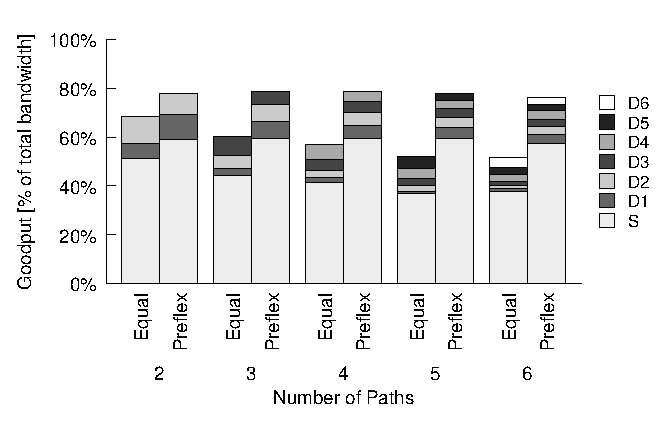
\includegraphics[width=4in]{figures/cate/diffbw}
    \caption{Goodput relative to $B$ achieved by each server for different capacity links.}
    \label{fig:goodputdiff}
\end{figure}

Where bottleneck bandwidth is unequal however equalisation proves inadequate. 
Once again comparing goodput (figure \ref{fig:goodputdiff}) we highlight two significant shortcomings of equalisation which \ac{PREFLEX} overcomes. 
Firstly, goodput for $S$ drops as $N$ increases. 
Unable to realize it is overloading a path, equalisation is reduced to sending traffic over each link at approximately the same rate as the most congested link. 
In contrast, \ac{PREFLEX} detects congestion and adapts accordingly. 
Secondly, the incorrect distribution of traffic due to equalisation in $S$ distorts the goodput of others servers. 
While in \ac{PREFLEX} goodput from $D_{1-N}$ is perfectly balanced, with equalisation traffic crossing the most congested links are directly affected by another domain's inability to distribute its traffic appropriately.
It may seem unfair to judge equalisation for cases where there is a mismatch in link capacity, however this mismatch between link weight and path capacity arises regularly as operators continue to adjust traffic engineering according to local conditions, with little thought spared for the impact this may have further downstream.

\begin{figure}
    \centering
    \includegraphics[width=3.2in]{figures/cate/duration}
    \caption{Mean average flow completion time for equal and differing bottleneck links.}
    \label{fig:duration}
\end{figure}

This impact is in turn perceived by users, who experience longer flow completion times, as shown in figure \ref{fig:duration}. 
In the equal bandwidth case the flow completion time is similar for both balancers.  
Where bandwidth differs however, \ac{PREFLEX} outperforms equalisation and maintains a stable performance when balancing over all six paths.  
This shows that the algorithm scales well as the number of available paths increases. 


\section{Conclusions}
\label{section:malawi:conclusion}

The focus of this work has been on elucidating the main factors that affect flow throughput, but which escape traditional TCP modelling based on end-to-end loss and delay. 
In particular, we explore the changing role of \emph{host limiting}, \emph{application pacing} and \emph{receiver shaping} in defining flow rates across five years of transit traces.
Our results show that for the observed link, over \emph{half} of all inbound TCP traffic can be ascribed to one of the aforementioned constraints.
We show that continuing OS upgrades have progressively lifted the artificial throughput constraints imposed by the host stack. In particular, windowscale negotiation for inbound traffic increased threefold in the observed period, covering over 80\% of all observed bytes by 2012; in addition, we show that buffer sizes have also shown continuing increases over time.

These developments have significantly improved throughput, in particular for smaller flows. However, we also found evidence of throughput limiting effects independent from available end-to-end capacity. This means that no amount of bandwidth will directly improve TCP rates for a considerable amount of traffic.
We show that application-driven techniques for chunked transfer are widely used, accounting for 40\% of all inbound traffic observed in 2011.
%, and that this behaviour is endemic to a wider range of stakeholders than in 2007.
Finally, we uncover evidence of significant receiver traffic shaping prior to 2011 based on the modification of the receiver advertised window in a bid to curtail congestion.
%Uncover evidence of receiver shaping during period of relative contention.



\chapter{A longitudinal analysis of \acs{TCP} traffic}
\label{chapter:malawi}

\renewcommand{\locfolder}{\chapfolder/malawi}
\section{Introduction}

% generic "failures are bad"
Despite being broadly designed for robustness, the current Internet architecture remains remarkably vulnerable to failures.
Managing faults effectively poses a significant operational challenge, in part because faults differ widely in both source and nature, potentially occuring at any layer of the stack and along any element along a path.

% neither is transport
\LOREM
\LOREM

% network methods
Given the commercial nature of the Internet, the onus of providing resilience has instead shifted to network operators.
Traditionally this has been achieved by overloading the routing architecture.
The deployment of real time applications with harder constraints on reliability coupled with better failure detection methods embedded in linecards have provided both the motivation and the means for achieving sub-second recovery within IGP networks \cite{}.
Even with reduced recovery times however, the transient effects of routing changes can still disrupt the forwarding path. 
Under such cases diverse proposals such as Fast Re-Route \cite{}, Loop-Free Alternate next hops \cite{} or Packet Re-cycling \cite{} can provide repair paths for use between the detection of a failure and the convergence of the routing process.

Unfortunately, such methods are rarely sufficient.
Firstly, their application is circumscribed to individual domains, and as such cannot provide end-to-end coverage in a federated, best-effort Internet.
Secondly, there are many faults which do not directly pertain to routing, such as middlebox misconfiguration or hardware malfunctions, and as such go undetected.
Finally, reparation often disregards and potentially disrupts the transport layer by causing out-of-order delivery of packets.

% why now. datacenter, SDN
\LOREM
\LOREM
\LOREM

% layout?
\LOREM
\LOREM


%Outside their networks however, operators are reduced to negotiating service level agreements with their own providers who are invariably unable to cater for such specialized demands \cite{}.
%Even if such terms were met, the Internet architecture provides limited visibility beyond one's own domain.
%This opaqueness, in addition to the fact that failures themselves may be distributed in nature \cite{}, severely limits the ability for a customer network to trace remote problems to a single source \cite{}.
%With no means to hold providers accountable for failures, there is little to enforce the terms of a truly end-to-end SLA.
%
%Unfortunately, such intradomain methods 


%Alongside this increased centralization of resources comes a heightened sense of accountability.
%The commercial nature of the agreements between customers and cloud hosting companies such as AWS \cite{} often involve the establishment of service level agreements.
%Even where such agreements are not explicit, such as the base option of tiered services such as Dropbox or Heroku, there is an inherent need to minimize the impact of outages -- non paying customers may be less demanding, but they are also less sensitive to the switching cost incurred in changing service provider.
%
%Unfortunately, the federated, best-effort nature of the Internet seemingly does not lend itself to such high expectations.



%Under such cases, a network operator is currently expected to detect, repair and recover from such faults.
%Detection often requires scale -- the reliability with which a fault can be identified relies on the proportion of traffic affected. 
%In many cases, faults affecting single flows may go undetected by the network.
%Once detected, reparation varies according to the nature and origin of the fault.
%For some cases, such as intradomain routing, this process is often automated and robust.
%For many others however, such as faulty hardware or misconfigured devices, recovery is difficult and error-prone.
%In either case, the amount of time expended in detection and repair can often preclude recovery, since most flows will terminate after successive timeouts.
%

%Fueled largely by economies of scale in both software management and hardware acquisition and maintenance, the emergence of cloud computing and content distribution networks has lead to a profound shift in Internet traffic.
%
%
%Whereas the advent of broadband connections init
%In contrast to the highly distributed nature of peer-to-peer software which 
%
%
%For one, never has so much been distributed by so few to so many.
%% AS dist graph
%% netflix
%
%\LOREM
%
%% Accountability, resilience

%All intervening equipment is subject to failure along a network path, with recovery time depending not only on \emph{what} happened, but also \emph{where}.
%Within their networks, operators are free to instrument and deploy arbitrarily complex tools to meet requirements. 
%This freedom has lead to a proliferation of proposed improvements in resilience for intradomain settings \cite{}.


%The establishment of SLAs for network availability have traditionally been prefered within the telecom industry in particular, and represent one possible approach to ensuring resilience. An alternative approach is offered by the end-to-end principle. 
%Since end hosts possess both inherent knowledge of application needs and fine-grained measurements on end-to-end path characteristics, the transport layer is often identified as a more natural fit for dealing with fault tolerance at an Internet scale.
%Both SCTP \cite{} and MPTCP \cite{} enable transparent fail-over through multihoming.
%In spite of providing significant features, neither is likely to be widely deployed in the near future: the former lacks critical middlebox support, while the latter is still undergoing standardization.
%Furthermore, the requirement for end-host multihoming has also posed a barrier to deployment.
%Finally, all transport approaches to fail-over confine knowledge of faults within an individual flow: each flow must detect failures independently, even when many flows are affected by the same fault.
%


% Transport is not the answer

% Can we do better with SDN?


%A default forwarding plane, corresponding to the label 0, must be defined and cater for all traffic destinations.
%As with existing routing infrastructure, this single default plane will suffice for most traffic.

%Invariably however, path failures will arise which may affect any number of flows.
%Rather than expecting the network to address end-to-end failures, hosts are allowed to proactively request an overlay plane from the network.





\section{Related work}
\label{section:malawi:related}

Despite their inherent value, longitudinal studies of Internet phenomena are rare. 
Over its short lifespan the Internet has been shaped as much by technological change as by political and commercial realities. 
This dynamic nature does not lend itself to observational studies where data must be collected and curated over long periods of time, and has resulted in a scarcity of relevant datasets. 
What few exceptions exist often stem from collaborative research efforts, such as CAIDA \cite{CAIDA} or Oregon Routeviews \cite{routeviews}. 
The usefulness of these datasets however can be severely affected by the need for data privacy. 
The dissemination of interdomain routing information, where no such requirement exists, has assisted in a wealth of research on wide ranging topics, from quantifying path diversity \cite{Oliveira:2009p203} to locating Internet bottlenecks \cite{Hu:2004p96}. 
In contrast, longitudinal datasets relating to passive measurements have nurtured a much smaller community of researchers often focusing on characterizing traffic \cite{Fontugne:2010p413}. 
Stripped of the locality contained within IP addresses however, researchers are left unable to relate these findings to a wider context.
Instead, cross-sectional studies characterizing traffic aggregated by location are frequently conducted under different contexts \cite{Ager:2011:WCC:2068816.2068870}, but lack the temporal perspective only longitudinal studies can afford. 
Efforts to characterize the spatial properties of traffic over time \cite{Dhamdhere:2011p428,Labovitz:2010:IIT:2043164.1851194,Cho:2008:OSC:1544012.1544024} have defined the changing of Internet topology and traffic alike but fall short of relating such shifts with their impact on relevant metrics such as loss or delay. 

% other work since
This chapter builds on a wealth of prior work on understanding Internet traffic and serves as a reappraisal of significant past contributions.
Flow characteristics and \ac{TCP} behaviour at large are subject to frequent reassessment \cite{Zhang:2002p85}.
Of particular relevance to the current work are passive studies which delve into the inner mechanisms of \ac{TCP}.
In \cite{Jaiswal:2004p242}, Jaiswal et al.\ infer the sender's congestion window by identifying the congestion control variant from the behaviour observed during loss recovery.
The use of separate state machines for each variant however proves unscalable given the many flavours of \ac{TCP} congestion control which have since been deployed.
In \cite{Lan:2006p566}, Lan et al.\ analyse flows according to size, duration, rate and burstiness and characterise the observed correlations for heavy-hitters specifically,
uncovering evidence of increased application influence on flow rates and burstiness and consequently suggest treating flow size and duration as independent dimensions.

One central aspect to the analysis of \ac{TCP} behaviour is the estimation of \ac{RTT} from packet capture data. 
In addition to SYN-based methods, Shakkotai et al.\ \cite{Shakkottai:2004p408} evaluate further techniques to estimate the \ac{RTT} of a unidirectional flow. 
The \textit{rate change} method establishes a relation between the \ac{RTT} and the increase in sending rate, assuming linear window increases during congestion avoidance. 
Unfortunately, this assumption no longer holds, both due to the proliferation of less conservative congestion control algorithms such as CUBIC \cite{Ha:2008p471}, and due to application-driven flow control. 
An alternative is the use of frequency-domain techniques \cite{Veal:2005p412,Lance:2005p565,Qian:2009p429}, which are a natural fit given the self-clocking nature of \ac{TCP}. 
However, a common difficulty with the application of spectral analysis is extracting the fundamental frequency which corresponds to the \ac{RTT} in the presence of noise. 
In applying the Fourier transform to inter-packet arrival times, for example, Qian et al.\ \cite{Qian:2009p429} note that less than half of all flows have distinguishable \textit{flow clocks}; likewise, the \ac{FFT}-based \ac{RTT} recovery was found to be unreliable even after pre-processing available data to enhance inherent periodicities.

% topological influence
Finally, it is important to elucidate what changes in traffic properties are intrinsic to \ac{TCP} and data transfer, and which ones arise from large-scale changes in the \ac{AS}-level topology of the Internet. 
In the decade since publication of \cite{Zhang:2002p85}, the Internet has undergone significant changes, shifting from a broadly hierarchical form to a flatter, more interconnected structure \cite{Labovitz:2010p175,Ager:2012p567}.
Given the longitudinal nature of this chapter and its focus on interdomain traffic in particular, the insights provided by these studies on the macroscopic effects of content consolidation are discernible within the studied dataset, and as such are a source of validation for many of the observations herein.

\section{Dataset}
\label{section:malawi:dataset}

This section provides an overview of the datasets used in this work and some of the data processing required before approaching the longitudinal study of Internet traffic rate limiting. We use the original, unanonymised traffic traces of the MAWI \cite{mawi} dataset, a set of daily traces from the WIDE backbone network which provides connectivity to universities and research institutes in Japan. Traffic is captured daily for 15 minutes starting at 14:00JST. Although this dataset extends back largely uninterrupted from late 2001, we focus on just over five years of data following a network upgrade to the monitored link on October 2006.

The monitored link carries mostly trans-Pacific commodity traffic between WIDE customers and non-Japanese commercial networks. 
We will refer to traffic towards WIDE as \emph{inbound} traffic, whereas traffic originating from within WIDE is referred to as \emph{outbound} traffic.

\begin{table}[!htp]
\scriptsize
\centering
    \begin{tabular}{r|cccccc}
        & & TCP data & \multicolumn{2}{c}{Traffic (TB)} & \multicolumn{2}{c} {Count ($\times10^3$)} \\
        Year & Days & flows (x$10^6$) & In & Out & AS & Prefixes \\
        \hline
        2006 & 91 & 20.52 & 0.43& 0.45 & 10.90 & 56.86\\
        2007 & 350 & 102.56 & 2.11 & 2.49& 17.21 & 113.79\\
        2008 & 358 & 112.26& 2.43 & 2.10& 24.74 & 156.54\\
        2009 & 364 & 113.97& 2.48 & 2.53& 19.71 & 143.87\\
        2010 & 365 & 113.70& 2.58 & 3.43& 20.38 & 148.03\\
        2011 & 358 & 114.74& 3.44 & 5.14& 19.99 & 140.56\\
        \hline
        Total & 1886 & 5777.55 & 13.50 & 16.14 & 34.12 & 341.22\\
    \end{tabular}
    \caption{\label{table:overview}Overview of traced MAWI dataset 
}
  \vspace{-3mm}
\end{table}

A preliminary overview of the dataset used is provided in table \ref{table:overview}. 
In total, 5.7 billion flows containing data are traced over five largely uninterrupted years; this represents approximately 30 terabytes of TCP traffic. For the purposes of this work, we will focus exclusively on inbound traffic, 60\% to 80\% of which originates from port 80, referring only to analysis of outbound traffic when providing a wider context for our findings.
Given the sender side plays a critical role in shaping traffic, analysing traffic for which the source is restricted to a small set of networks within Japan would be of limited use in accurately depicting traffic trends at large.
We instead fix hosts within Japan as sinks, thus sharing a similar perspective on inbound traffic as many other networks. 

\subsection{Tracing TCP Metrics}

All TCP flows are reassembled and analysed for each daily trace.
In addition to the five tuple used to define each connection, we impose two additional restrictions: a contiguous sequence number space and a three minute timeout. These restrictions are helpful to deal with port reuse and unterminated flows respectively.  
Although the total number of TCP flows increased dramatically in 2011, the number of flows \emph{for which data payload was seen} has remained stable, averaging over 100 million data flows traced per year.  

There is much prior work with regards to reconstructing TCP flow from passive measurements and using this information to understand the end-to-end properties of traffic \cite{firstRTT,Jaiswal:2007p233,Rewaskar:2007p195,Shakkottai:2004p408}. However, the MAWI traces impose two constraints which require careful consideration, and ultimately led to the use of a custom TCP tracer. 
The first one is the proportion of bidirectional flows, that is flows, where both forward and reverse path are seen. 
In the dataset used this fluctuates between 40\% and 60\% over five years.
Most available TCP tracers either ignore or are inadequate at processing unidirectional flows. 
The second one is the short duration of each individual trace file. 
At only 15 minutes of line-rate data capture per day, it is wasteful to ignore flows which are not complete. Although the number of flows for which a SYN and FIN in either direction is observed has remained consistently high until late 2011, these flows are normally \emph{mice}, i.e. flows that tend to be brief and which carry little traffic individually. In contrast, most \emph{elephants} (flows that carry significant traffic individually) have durations that exceed that of each trace file. 

%rtts traced
%While many metrics are extracted for each flow, for the purposes of this paper we will focus only on detailing how we collected delay and loss.
%Passive RTT estimates, calculated as the offset between a data packet and its respective acknowledgement, require both directions to be observed at the measurement point. 
%This provides delay estimates between the measurement point and the receiver, as illustrated in figure \ref{fig:synrtts}. 
%For flows where data is transfered in both directions, we will obtain in effect two separate estimates, $RTT_{m2a}$ and $RTT_{m2b}$, illustrated in figure \ref{fig:synrtts}. 
%Together they form the total end-to-end delay experienced by end-hosts. 
%For the remainder of this paper, the term RTT will refer to delay between our measurement and destinations outside WIDE. 
%We discard the delay between measurement point and hosts within WIDE for two reasons. 
%It is both negligible for a large proportion of traffic, which is highly concentrated within the Tokyo metropolitan regions and immediate surroundings, and extremely large for a very small subset of hosts located outside Japan, as WIDE has in the past acted as a provider to academic institutions in Indonesia through a satelite uplink. 
%By decoupling both directions we focus purely on the changes in delay to locations outside Japan. 
%This incurs a reduction in the range of destinations for which we can obtain estimates - only bidirectional traffic can be traced this way. 
%For the set of destinations we will study in this paper, we shall show that this reduction is small. 
%For tracking delay changes for unidirectional traffic for other purposes, MALAWI includes RTT estimates extracted from the SYN exchange.

Loss is inferred by accounting for \emph{retransmissions} in the upstream data and \emph{out-of-order packets} in downstream data; for the remainder of the paper we will refer to the \emph{end-to-end loss} as the sum of out of order and retransmitted data bytes over the total data bytes in a given direction.
% XXX: remove RTT ref?
%Tracking both retransmissions and out-of-order packets accurately requires a reliable RTT estimate, which can only be obtained for bidirectional flows. We forfeit some precision by not taking this into account, as we wish to be consistent in how we estimate both metrics independently of the type of flow and aggregation. 
Pragmatically, we found this to be an adequate indicator of loss --- with the exception of \emph{hanging} TCP connections. 
In these cases where connectivity is lost, a host will proceed to retransmit packets while performing an exponential backoff. 
Although this results in negligible overall traffic, it can significantly skew the inferred loss ratio for uncommon destinations for which little traffic exists. 
To account for these cases, we imposed a 3-second timeout on retransmissions after which we consider the congestion feedback loop to be broken. 

Each daily trace in the dataset is processed from a packet level capture into a collection of flow level statistics. 
This gives us insight into the end-to-end characteristics of traffic. However, since a core objective of this work is to augment this time-based information with data describing the endpoints of each flow, aggregating by location is also required. 

\subsection{Aggregating by Location}

Location information is added by mapping the original source and destination IP addresses to its geographical and topological counterpoints. 
We use the \emph{routeviews} archives to reconstruct the mapping between each IP and both AS and network prefix; bi-hourly dumps of BGP RIBs are available in the WIDE archives since mid 2003. 
We reconstruct a daily RIB based on the views provided by contributing ASes, in particular IIJ and APNIC. 
Since exact routes are not disclosed (there is no record of local policy), we have no knowledge of the route taken by packets; this of course does not hinder our ability to consistently map IPs to ASes. While discrepancies in AS destinations exist between different routeviews contributors, we note that this happens almost exclusively on prefixes for which no actual traffic is seen. 

Mapping IP to country is done through the use of GeoLite \cite{maxmind}, a commercial geolocation database. 
While the accuracy of this solution is often disputed, we are not overly concerned with locating traffic at a fine granularity. 
We will mostly focus on tracking traffic by country and, for larger countries such as the U.S, by region, in order to capture shifts over time.
GeoLite proves adequate on both counts.
The archive for geolocation data only extends to 2009, before which we must rely on the earliest match. 
Additionally, we verify if the destination or source AS have maintained the same administrative mapping up until mid 2009 in the relevant RIR (regional internet registry) archives; otherwise, we do not associate a flow to a geographical location.
% bridging paragraphs to save space.
After associating flows to country, region, AS and network prefix for both source and destination IPs, we aggregate flow statistics over each location identifier. 
This generates a daily collection of location identifiers and associated flow properties, from which we can sketch the geographic and topological properties of the dataset over time.

\section{Methodology}

Providing a macroscopic view on where traffic originates from, and in what quantity, can be achieved by simply binning packets into flows and accumulating byte counts over geographical or topological locations. 
Uncovering application layer characteristics (i.e. \textit{how} traffic is sent) is a more complex problem that requires additional methods to reverse engineer transport behaviour.
The aim of this section is to describe a process which distinguishes those flows which have their throughput limited by mechanisms other than the usual \ac{TCP} response to loss and delay.
Each flow can be characterized as being either application paced, in which the sending application is limiting the data provided, host limited, whereby local constraints at either end host cap throughput, or receiver shaped, in which an artificial constraint is imposed by either a middlebox or receiver.

The classification proceeds in stages. 
Before classification, it is necessary to reconstruct the RTT of the flow if the flow is not bidirectional.  
This is achieved in section \ref{subsection:malawi:PeriodicEnhancement}. 
Because the sender's TCP state machine cannot be directly observed it is necessary then to estimate the size of the congestion window by observing the number of unacknowledged bytes in flight (\textit{flight size}).
This reconstruction is described in section \ref{subsection:malawi:flightAggregation} and provides the basis for flow classification. 
Flows are then checked in turn to see if they are application paced, host limited or receiver shaped and classified as belonging to the first of these classes for which they fulfill the necessary conditions.
Flows in none of these classes are either limited only by the network (delay or loss conditions) or are insufficiently large to trigger any further constraints.

\subsection{RTT Estimation}
\label{subsection:malawi:PeriodicEnhancement}

Building on prior work presented in section \ref{section:malawi:related}, this section proposes an algorithm that scalably recovers the RTT from one-directional traffic traces. 
% XXX: below implies microflights were used, but these aren't described (remove as appropriate)
Although \ac{RTT} estimation is a difficult problem, simplifying assumptions can be made.
For the \ac{MAWI} dataset most \acp{RTT} are relatively large, with the closest neighbouring country, South Korea, roughly 40ms away.
By only processing bidirectional traffic from Japan, the expected \ac{RTT} range can be reduced for all other traffic.
The recovery mechanism then enhances the natural periodicity of traces and scalably constructs flights associated with specific application and protocol behaviour.
In the following the mechanisms required by these two goals are described. 
%
% Why does this work?
%
In normal operation, many \ac{TCP} operations involve request-response cycles between two endpoints in which the \ac{RTT} $T$ provides a natural \emph{clock}.
Hence, the most natural way to estimate \ac{RTT} from \ac{TCP} traces is to correlate requests and responses exchanged in both directions. 
If only one direction of data is observed however, $T$ cannot be directly observed. 
Instead, it must be estimated from the way in which \ac{TCP} packets cluster in time due to the batching of request-response operations.

The \ac{TCP} \ac{cwnd} determines the number of unacknowledged bytes that a \ac{TCP} flow may maintain at any point in time. 
This can be referred to as \emph{bytes in flight} because they are in transit between the sender $S$ and the receiver $R$; an equivalent definition applies for the number of \emph{packets in flight}. 
Once $S$ has transmitted \ac{cwnd} data bytes, it will refrain from transmitting more until either some bytes are acknowledged by $R$ or \ac{cwnd} is increased by the sender. 
In the absence of losses, neither of these events can happen until a \ac{TCP} \ac{ACK} is received; this immediately reduces the number of unacknowledged bytes, but may also lead to a significant \ac{cwnd} increase (during e.g. \emph{slow start}). 
% XXX: number of unacknowledged bytes reduced, or CWND?
In the presence of losses, however, bytes can be re-sent if a packet is timed out and considered lost; in this case, the number of unacknowledged bytes is reduced.

%
% What is our main contribution, algorithmically speaking?
%
The main difficulty associated with one-sided TCP flow reconstruction is as follows.
Let $t_1, t_2, \ldots$ be a set of times at which packets $p_1, p_2, \ldots$ were observed at $S$ en route to $R$.
Suppose that a packet $p_j$ of size $b$ is observed at time $t_j$.
In addition, suppose that approximately one RTT $T$ later, the sender $S$ receives an ACK $a_j$ from $R$ for the $b$ bytes of $p_j$.
At this point, the TCP stack in $S$ will decrease the number of unacknowledged bytes by $b$, thus opening the possibility for sending additional traffic to $R$.
This can lead to another packet $p_k$ to be transmitted; let this packet be observed at time $t_k$ as it is sent towards $R$.
Assuming that processing delay is insignificant, the RTT experienced by $p_j$ can be approximated as $T \approx t_k - t_j$.
Now consider what happens if packets are only observed in the $S \rightarrow R$ direction.
Under such conditions, it is not possible to ascertain whether $p_k$ was sent explicitly as a result of $S$ receiving the unobserved \ac{ACK} $a_j$, or whether it was sent as a result of an \ac{ACK} $a_i$ associated with a previous packet $p_i$ rather than with $p_j$.
If, however, a packet $p_l$ is eventually observed that did result from the reception of $a_j$, the \ac{RTT} can be estimated as $T \approx t_l - t_j$ with $t_l > t_k$.
Following this same reasoning, approximately one \ac{RTT} later a packet $p_m$ will be observed for which $2T \approx t_m - t_j$; this can potentially continue for as long $S$ has data to send and $R$ continues sending \acp{ACK}.
This is the underlying reason that \ac{RTT}-related periodic regularities arise when considering the timestamps of observed packets \cite{Qian:2009p429}.

The reasoning above is at the heart of the proposed algorithm to improve \ac{RTT} recovery by enhancing packet stream periodicity. 
Assume that a packet $p_j$ is observed at time $t_j$. 
Considering the set $\mathcal{T}_j$ of all values of $\Delta t = t_k - t_j$ for every $k > j$, it is apparent that it will include estimates not only for the \ac{RTT} $T$, but also for all its multiples $2T, 3T, \ldots$ 
If $t_l-t_k \approx T$ and $t_k - t_j \approx T$ then it follows that $t_l - t_j = 2T$, and this value will also be included in $\mathcal{T}_j$. 

By maintaining a set $\mathcal{T}_j$ for every packet $p_j$ observed, at least some of its values will correspond to estimations of multiples of the \ac{RTT}. 
It then follows that by creating a set $\mathcal{T}$ that includes values calculated starting from every packet $p_j$ so that $\mathcal{T} = \cup_j \mathcal{T}_j$, numerous estimates for $2T, 3T, \ldots$ will also be included. 
Hence, the probability density function $H(t)$ of the values in $\mathcal{T}$ should show peaks around multiples of the \ac{RTT} (see Figure \ref{fig:histogram}). 

\begin{figure}
  \centering
  \includegraphics[width=0.8\textwidth]{figures/malawi/rttbin.pdf}
  \caption{$H(t)$ for flow displayed in Figure \ref{fig:hostlimited}. The horizontal line delimits $\overline{H}$ while the highlighted bin denotes the bidirectional RTT estimate.\label{fig:histogram}}
\end{figure}

%
% Explain why did we use FFT
%
The algorithmic recovery of $T$ from $H(t)$ presents additional challenges. 
In particular, $H(t)$ may include a large number of \ac{RTT} multiples, and a peak will be found for all of them. 
Crucially, all these peaks may be of comparable magnitude, complicating the task of selecting a single peak.
Moreover, these peaks need not be very pronounced, with histogram bins in close proximity of the peaks have very similar values as the peak itself. 
As such, taking \ac{RTT} candidates directly from $H(t)$ may result in a large set of similarly-valued bins situated around a peaks at multiples of the \ac{RTT}. 

Three recovery algorithms for $T$ are attempted.
First, as a baseline, the highest peak in $H(t)$ is selected as a candidate for $T$. 
In addition, expanding upon the work of Qian et. al. \cite{Qian:2009p429} a frequency-domain representation of $H(t)$ is used to identify $T$. 
This is done by selecting the highest peak of $|\hat{H}(\omega)|^2$, the \emph{energy spectral density} of $H(t)$ (i.e. the norm squared of the Fourier transform of $H(t)$). 
Finally, a custom utility-based technique that operates directly on $H(t)$ is proposed which achieves superior performance to both of the aforementioned methods.

%\subsubsection{FFT-Based RTT Recovery}
%We extract periodicity information from $H(t)$ by looking at $\hat{H}(\omega)$, the \emph{energy spectral density} of $H(t)$. Formally, $\hat{H}(\omega)$ is defined as the norm squared of the Fourier transform of $H(t)$, so that $\hat{H}(\omega) = |\mathcal{F}(H(t))|^2$. Using $\hat{H}(\omega)$ markedly improves the quality of our RTT estimation because the frequency peak corresponding to the RTT usually accounts for a much larger proportion of the total frequency domain energy than other peaks in $\hat{H}(\omega)$, leading to a much simpler discrimination of the true RTT. However, due to RTT changing during the lifetime of a flow, and also due to the expected noise associated with real-life data sources, $\hat{H}(\omega)$ can also occasionally include large peaks at frequencies unrelated to the RTT. In order to filter these out, we take a set of 10 frequency candidates from $\hat{H}(\omega)$, and use their associated periods as RTT candidates in our flow reconstruction algorithm (see Section \ref{
%subsection:malawi:flightAggregation}). We then select that RTT candidate which exhibits the smallest error, that is, that one which yields closest agreement with observed data.

%
% Algorithmic hacks
%
%To streamline our algorithm for streaming use, we use the following heuristics and approximations. Firstly, we define a range $[T_{\min}, T_{\max}]$ representing the range over which we find the RTT values of interest. Then, for each packet $p_j$, we build a subset $\mathcal{T}_j'$ of $\mathcal{T}_j$ by including all values of $t_j - t_k < T_{\max}$. We then generate $\mathcal{T}' = \cup_j \mathcal{T}_j'$ and approximate $H(t)$ by considering a histogram of the values in $\mathcal{T}'$. As usual, we do this by counting the frequency with which its values are observed in the ranges $[0,\tau)$, $[\tau, 2\tau)$, $[2\tau, 3\tau), \ldots$ where $\tau$ is the time resolution required. 


\subsubsection{Utility-Based RTT Recovery}
\label{sect:utilityBasedRecovery}

This method relies not on the identification of periodicities, but on explicitly matching experimentally found signatures. 
To this end, we consider the peaks of $H(t)$, which are then considered RTT candidates.  
However, trivial discriminators (such as simply selecting the highest peak) are not reliable. 
In this case, it was found experimentally that repeatable peaks and troughs also occur at multiples and sub-multiples of $T$, with the most important ones being $\frac{T}{3}$, $\frac{T}{2}$, $T$ and $2T$. 
We design this detection algorithm around the idea that a given pattern of peaks and troughs can identify $T$.

If we define $\overline{H}$ as the mean height of $H(t)$, we can define a per-peak utility function $p(t)$ so that 
\begin{equation*}
p(t) = 1.0 - \exp\left(-2.0 \left(\frac{H(t)}{\overline{H}}\right)\right) \mbox{.}
\end{equation*}
This function has several advantageous properties: it is 0 if $H(t)$ is zero, 1
if $H(t)$ is infinite, and $0.5$ if $H(t) = \overline{H}$.  In other
words it is a measure of the \emph{peakiness} of the data, with $p=1$ identifying
an infinitely high peak, $p=0$ identifying an empty histogram bin (trough), and $p=\frac{1}{2}$ 
implying that $H(t)$ is of exactly average height at that point. We can then score each candidate using the following utility function:
$$
P(t) = 1.5 p(t) + p(2t) - p\left(\frac{t}{2}\right) - p\left(\frac{t}{3}\right).
$$
That is, the candidate RTT $t$ scores highly if it is itself a peak, if it has a peak
at a multiple $2t$, and if it also manifests troughs at submultiples $\frac{T}{2}$ and $\frac{T}{3}$.
The factor of 1.5 was added after observations
showed that the peak at $T$ was the most important factor in determining
whether a candidate was the true RTT. Similarly, additional multiples and submultiples 
were excluded as they showed very limited discriminating power experimentally.

\begin{figure}
  \centering
  \includegraphics[width=0.8\textwidth]{figures/malawi/rttcomp.pdf}
  \caption{Accuracy of RTT estimator when compared to the median value of bidirectional estimate.}
\end{figure}

\subsubsection{Comparing RTT Recovery Algorithms}
\label{sect:comparingRecoveryAlgos}
As described in Section \ref{subsection:malawi:PeriodicEnhancement}, $H(t)$ is calculated in such a way that RTT periodicity is amplified. 
This means that FFT-based techniques could potentially perform better on $H(t)$ than on the packet stream with no pre-processing. 
However, this is complicated not only because $H(t)$ contains periodicities at multiples of $T$, but also discontinuities that generate harmonics at frequency multiples of the RTT fundamental. 
Hence, although the FFT $|\hat{H}(\omega)|$ of $H(t)$ is much cleaner than that of the packet interarrival time series on its own, its maximum peak rarely coincides exactly with the RTT clock (this corroborates reports by Qian et al \cite{Qian:2009p429}). 
Thus, applying the FFT leads to another \emph{peak detection problem} in which the RTT fundamental needs to be extricated from its harmonics and sub-harmonics. 
The trivial solution to this problem, the application of a bandpass filter around the RTT frequency, is of course unfeasible because the bandwidth and 
centring of such a filter depend on the RTT which is itself unknown.
The utility-based algorithm described in Section \ref{sect:utilityBasedRecovery} can hence be applied in either the time domain or the frequency domain; we chose to do it on the former on the interest of expediency and lower computational cost.

\newcommand{\RTTHeader}{Below & Above}
\newcommand{\SmallFlowName}{\textless 10MB}
\newcommand{\LargeFlowName}{\textgreater 10MB} 
\begin{table}
\footnotesize
\centering
\begin{tabular}{ p{1.5cm} p{1.2cm} p{0cm} p{.6cm}p{.6cm} p{0cm} p{.6cm}p{.6cm}}
& & & \multicolumn{2}{c}{Peak} & & \multicolumn{2}{c}{Utility-based} \\
\cline{4-5} \cline{7-8}
& Flow size & & \RTTHeader & & \RTTHeader \\
\cline{4-5} \cline{7-8} 
\multirow{2}{*}{Receiver side}  & \SmallFlowName && 4.31 & 9.13 && 4.58 & 6.35
\\ 
                                & \LargeFlowName && 6.72 & 6.43 & 4.97 & 5.33
\\
\multirow{2}{*}{Sender side}    & \SmallFlowName && 2.94 & 8.37 && 3.29 & 4.80
\\
                                & \LargeFlowName && 6.41 & 9.06 && 5.40 & 11.06
\\
\end{tabular}
\caption{\label{table:rttRecovery}Performance of RTT recovery algorithms}
\vspace{-3mm}
\end{table}

The performance of the analysed RTT recovery mechanisms is presented in Table \ref{table:rttRecovery}, that shows the percentage of total flows below and above the RTT range given by the bidirectional estimates.
We separate things for \emph{inbound} traffic (where we are positioned at the receiver side) and \emph{outbound} traffic (where we are positioned at the sender side). The utility-based algorithm is particularly useful to address RTT underestimation for flows over 10MB in size, which is our main objective since precisely that kind of estimation error would interfere with our ability to correctly decouple application behaviour from RTT-scale dynamics.


%For the most part, the utility based method improves on underestimation, which is our main objective since that would interfere with our flight reconstruction (i.e. generate lots of gaps).
%The exception (kind of) is traffic from the sender side, which in our training set (one week per year), had quite a lot of host limited traffic (paced out, no signal to recover).
%In this case, not a problem, since if the flow is long enough multiples of the RTT will still reveal host limitation, but will give us a smaller window..


\subsection{Flow Classification}
\label{subsection:malawi:flightAggregation}

One fundamental precondition to decouple the influence that network loss, host configuration and TCP behaviour has on the throughput experienced by a flow is the reconstruction of the congestion window behaviour of TCP flows on the basis of observed data. 
Unfortunately, the congestion window value is internal to the sender's TCP state machine and may not manifest itself in the absence of sufficient data from the application layer. 
A more easily observed quantity which serves as a reasonable proxy for the congestion window is the number of unacknowledged bytes in flight, henceforth referred to as the \textit{flight size}, which can be derived given an accurate estimate of the end-to-end delay.
The evolution of both flight size and RTT can in turn be used to ascertain to what extent throughput is regulated by limitations imposed at different layers of the networking stack.

% definitions
Given a candidate RTT, we can aggregate a stream of packets with arrival times $t_1, t_2, \ldots$ into a stream of \emph{flights}. 
Intuitively, a flight is a clustered subset of a TCP flow which exhibits its own temporal coherence; alternatively, it can be though of as a series of consecutive packets that were (roughly) generated by the sender as a response to the same protocol operation. 
A flight $f_i$ that begins
with the $j$th packet and ends with the $k$th is defined to have a \emph{total flight time} $\tau_i = t_{k+1} - t_j$. 
The algorithmic selection of initial and final packets in such a way that the resulting flights are indicative of TCP behaviour remains an open problem. 
Since we assume that the RTT provides a natural time frame for the operations of TCP, in the algorithm presented in this work, given an initial packet $\pi_j$ and an RTT estimate $T$, the $k$th (and final) packet is selected to minimise \emph{the flight time error} $e_i = |T - \tau_i|$. 
This mechanism follows closely the methodology described in \cite{Zhang:2002p85}, with the exception that we do not attempt to define flights as being both adjacent and disjoint; rather, we decompose flows into a stream of potentially overlapping flights. 
This helps the algorithm mitigate the deleterious effects of small deviations in the estimated RTT, which alters the properties of each flight. 
Furthermore, since the flight size is continuous in time, it makes little sense to restrict ourselves to a single sample per round trip time.

Having obtained flight information from each flow, we next consider what is the predominant factor that affects its throughput. 
Within the context of TCP, we classify flows as being artificially constrained by three distinct processes: \emph{application pacing}, \emph{host limited} and \emph{receiver shaping}.

\begin{figure}
\centering
  \centering
  \begin{subfigure}{1.0\linewidth}
    \includegraphics[width=1.0\textwidth]{figures/malawi/youtube.pdf}
    \caption{Application paced. \label{fig:youtube}}
  \end{subfigure}\\
  \begin{subfigure}{1.0\linewidth}
    \includegraphics[width=1.0\textwidth]{figures/malawi/hostflow.pdf}
    \caption{Partially host limited. \label{fig:hostlimited}}
  \end{subfigure}\\
  \begin{subfigure}{1.0\linewidth}
    \includegraphics[width=1.0\textwidth]{figures/malawi/awnd.pdf}
    \caption{Receiver shaped. \label{fig:awnd}}
  \end{subfigure}
  \caption{Flight size over time for flows affected by different artificial constraints. \label{fig:kindsOfFlowEffect}}
\end{figure}


\subsubsection{Application Paced Flows}
\label{sssec:app}

A flow whose throughput decreases because it has no outstanding data to send is temporarily limited by the application. 
Flights can be identified as being \emph{application limited} if terminated with a packet smaller than the maximum segment size (MSS) and followed by an inter-arrival time greater than the RTT, as consistent with \cite{Zhang:2002p85}. 
The underlying reason for this defintion is that most TCP implementations will wait some time for subsequent bytes to be written to the socket if the next packet to be sent is smaller than the MSS, unless the TCP\_NODELAY option is set \cite{nagle1984rfc}.

A flow with \emph{application limited} flights however is not necessarily \emph{application paced}. In practice, all flows for which the final packet is observed contain at least one such flight.
For the purposes of our work, we are focused on identifying cases in which throughput is predominantly determined by application behaviour.
One such example is illustrated in figure \ref{fig:youtube}, in which a stream is delivered by periodically writing blocks to the sending socket.
The resulting network-level behaviour is distinct from traditional congestion control: short bursts are interspersed with protracted silence.
Application limited flights, which terminate on non-MSS packets, are highlighted at the end of each burst.

This behaviour is in stark contrast to that exhibited in figure \ref{fig:hostlimited}, where distinct transfers are multiplexed on top of a single transport association over time.
From the perspective of the network, there is little to distinguish the behaviour of such traffic from independent TCP flows.
Application paced connections such as Youtube traffic however exhibit a degree of regularity which can potentially be exploited by the network in predicting demand or smoothing bursts.

In order to identify such recurring behaviour, we identify flows as being \emph{application paced} if the period between bursts terminated by \emph{application limited flights} is consistently under 10 seconds and the standard deviation of the intermediate pauses is under one second.
This definition in particular purposely ignores flows which exhibit long silence periods due to user interaction, and follows closely the behaviour historically associated to Youtube streaming in particular.

\subsubsection{Host Limited Flows}
\label{sssec:host}

Given sufficient bandwidth and traffic to send, a flow may encounter local constraints at either end-host which cap its throughput. 
For instance, the buffer space allocated on both the sender and receiver side is often pre-configured, and it is common practice to tune these values down on popular servers and managed infrastructure in a bid to conserve memory or bandwidth.
A receiver is also limited in the window size it can announce to the remote sender; if the windowscale option \cite{jacobson1992tcp} is not negotiated during the TCP handshake, the advertised window cannot exceed 64KB.

In both cases, a local decision by either host can determine the upper bound of the flow rate.
These \emph{host limited} cases are characterised by a constant window size over time.
The methodology described for flight aggregation at the beginning of this section typically generates a large number of flights, representing many likely combinations given a base RTT estimate.
In order to identify the flat-lined behaviour of a host limited flow, we first filter the flight stream to remove some of the uncertainty derived from small fluctuations in the RTT.
We then select the maximum flight size observed for each RTT interval, and declare a sequence of flights to be host limited if the same maximum was observed over six consecutive RTTs (this is twice the period suggested in \cite{Zhang:2002p85}).
In practice, increasing the period over which the maximum window size is tracked allows us to more accurately discern between host limited behaviour and more conservative bandwidth probing, such as that performed during the convex phase of TCP CUBIC \cite{Ha:2008p471}.

A flow may be host limited for only brief periods of its lifetime, as illustrated in figure \ref{fig:hostlimited}.
To filter out such cases where host limitations are not the predominant factor in defining flow throughput, we further enforce that in addition to host-limited flights, the average window size must over a flow lifetime should be within 10\% of the inferred host limit, which is not the case in figure \ref{fig:hostlimited}.

In practice, flows can exhibit both application pacing and host limitations, with bursts being sent at a capped window size followed by application pauses.
In such cases, a flow will still be classified as being \emph{application paced} if it meets the requirements set out in the previous section, as doing so provides evidence that it controls throughput in spite of the degraded performance provided further down the stack. 
This line of reasoning applies equally to the occurrence of sporadic loss; so long as block delivery is ensured within the timeframe dictated by the application, it remains in control.

\subsubsection{Receiver Shaped Flows}
\label{sssec:rec}

A flow which is neither \emph{application paced} or \emph{host limited} can still be artificially constrained by flow control (rather than by congestion control).
Traditionally, in TCP the sender is responsible for regulating throughput. 
However, the receiver can also shape throughput by manipulating the \emph{advertised window} announced on every acknowledgement.
Such receiver-window auto-tuning has been available on Windows operating systems since Vista \cite{vistaReceiveWindow}, and can also be leveraged by middleboxes in order to throttle inbound traffic \cite{appEx}.

In order to evaluate the potential impact of such behaviour, we further propose a heuristic to identify receiver-shaped traffic.
For flows in which both directions of traffic are observed it is possible to correlate the evolution of the advertised window with the size of reconstructed flights.
Figure \ref{fig:awnd} displays an example of a receiver-shaped connection, in this case throttled by an intermediate middlebox.
Since the advertised window may be fluctuating, it is not always obvious which of the many updates were effectively applied by the sender as successive values supersede each other.
An example of a reconstructed flow which is subjected to receiver shaping is displayed in Figure \ref{fig:awnd}.

For flows in which both directions are observed, it is possible to classify flights as being receiver-shaped if there is a statistically significant correlation between the advertised window size and the maximum flight size observed.
Harnessing the stream filtering used in detecting host limited behaviour, we perform such analysis over a sliding window of 10 RTT intervals.
A flight is flagged as being receiver shaped if the correlation between receiver window and flight size is statistically significant; a flow is considered to be predominantly receiver shaped if over half of its flights are flagged as such.
We do not perform this covariance analysis on flights which contain out-of-order or retransmitted packets. 
In these cases, both the receiver and sender window sizes are correlated \emph{by definition}. 
In the former case, the receiver buffer will temporarily fill expecting the next packet in sequence, in the latter case, TCP will reduce its window.

Given that receiver shaping classification requires correlating information in both directions of a TCP connection, it will come as no surprise that the absence of the reverse path can introduce false positives into our measurements. 
This happens because any given flow might be receiver shaped in such a manner that the heuristic erroneously attributes its behaviour to host limitations. 
In the absence of additional evidence, this misclassification is difficult to detect explicitly. 
Instead, we calculate the ratio of receiver shaped flows which would have been incorrectly identified if the reverse path were not observed. 
This error rate can then be used to evaluate the accuracy of classifier results.

\section{Performance Analysis}
%4.1) Balancing between two paths with high loss using fixed time unit
% using only loss-based balance in a simple regime where that works.
% Show how this converges quickly when one path suddenly gains
% background traffic (and hence loss).
%4.2) Balance between several paths with high loss and fixed time unit
% in simple regime where that works.
%4.3) Introduce experiment where equi-path is needed for probing and
% conservative is needed for low loss regime.
%4.4) Introduce experiment where time-scale tuning is needed to get
% good assessment of loss in low traffic regime.

We evaluate \ac{PREFLEX} through simulation in ns-3 \cite{ns3}. 
Since \ac{PREFLEX} balances traffic using loss rather than load, there is a need to emulate the end-to-end behaviour of traffic. 
This proves more challenging than analysis of existing traffic engineering proposals which typically only focus on adjusting load, since we wish to verify the impact of \ac{PREFLEX} on end-user metrics. 

\subsection{Methodology}
\label{section:methodology}

For all simulations we will use the topology displayed in figure \ref{fig:topo}. 
The topology links a client domain $C$ to a server domain $S$ through $N$ paths with equal bottlenecks $L_i$, and total bandwidth $B=\sum{L_i}$. 
While a domain is represented as a single entity in figure \ref{fig:topo}, each domain is composed by a traffic generator connected to a router. 
Client $C$ generates $G$ simultaneous \ac{HTTP}-like requests (or ``gets") from $S$ according to a specified distribution, described at the end of this section. 
As traffic flows from $S$ to $C$, the router within $S$ is responsible for balancing traffic over all available paths.

\begin{figure}
    \centering
    \includegraphics[width=2.5in]{figures/cate/topo}
    \caption{Simulation topology}
    \label{fig:topo}
\end{figure}

Across simulations, as the number of paths increases, total bandwidth $B$ and the number of simultaneous requests $G$ is fixed. 
In this manner we wish to analyze how \ac{PREFLEX} balances traffic as the granularity with which it can split traffic becomes coarser.

Since we are interested in evaluating how \ac{PREFLEX} shifts traffic in response to loss, we introduce additional ``dummy" servers $D_i$ which are connected to $C$ through a single path. 
We partition the total simulation time $T$ into $N+2$ intervals starting on $s_i$, in which $s_0$ and $s_{N+1}$ have no traffic to $D_i$. 
Starting at time $s_i$, client $C$ generates $g_i$ requests to $D_i$ according to the same distribution as used to server $S$. 
All requests to $D_i$ end at time $s_{N+1}$. 
Equation \eqref{eq:si} sets the start time $s_i$ for requests to $D_i$ as a function of total simulation time $T$ and number of paths $N$. 
Likewise, equation \eqref{eq:gi} sets the number of simultaneous requests $g_i$ to $D_i$ as a function of $G$, the total number of requests to $S$, and $N$.
\begin{equation}
s_i = T\frac{i}{N+2}
\label{eq:si}
\end{equation}
\begin{equation}
\theta_i = \frac{\frac{1}{N+1-i}}{\sum{\frac{1}{N+1-i}}},  g_i = G\theta_i.
\label{eq:gi}
\end{equation}

Figure \ref{fig:demand} illustrates the number of simultaneous gets from $C$ to $D_i$ for $N=2$ (used in the example shown in figure \ref{fig:two}) and $N=4$. 
Generating cross-traffic in this manner serves two purposes. 
Firstly, $\sum{g_i}=G$, so independently of the number of concurrent paths, the maximum load in the system is $2G$. 
However, as the number of paths increases, the fluctuation in load for each path becomes smaller, and so we will stress the sensitivity with which \ac{PREFLEX} balances traffic. 
Secondly, the number of requests for each $D_i$ over time is the same. 
Over timescale $T$, equalisation appears to be an acceptable strategy, however within each interval we will show it performs poorly achieve consistent behaviour. 
This is a fundamental limitation of offline traffic engineering, which is calculated over very long timescales and is unable to adapt as traffic routinely shifts.


\begin{figure}
    \begin{subfigure}[b]{.5\linewidth}
        \centering
        \includegraphics[width=2.25in]{figures/cate/dummy2-crop.pdf}
        \caption{$N=2$}\label{fig:1a}
    \end{subfigure}%
    \begin{subfigure}[b]{.5\linewidth}
        \centering
        \includegraphics[width=2.25in]{figures/cate/dummy4-crop.pdf}
        \caption{$N=4$}\label{fig:1b}
    \end{subfigure}
    \caption{Number of requests from $C$ to cross traffic servers $D_i$ for different values of $N$}
    \label{fig:demand}
\end{figure}

We now specify the settings common to all simulations, including those previously shown in figure \ref{fig:two}. 
Total simulation time $T$ is set to $1200$ seconds, while total bandwidth $B$ is fixed at $240$Mbps. 
The number of requests $G$ sent from $C$ to $S$ is set to 240. 
Upon completing, a request is respawned after an idle period following an exponential distribution with a $15$s mean. 
Transfer size follows a Weibull distribution with an average value of $2$MB. 
These values attempt to reflect traffic to a single prefix with a file size that mimics the small but bursty nature of web traffic, which does not lend itself to being balanced by the end-host. 
\ac{PREFLEX} is configured with $\beta_E = 0.05$, $\mu_{min}=0.01/N$ and $\delta=0.005$.

\subsection{Varying bottleneck distribution}

We start by examining the case where all bottlenecks share the same bandwidth, $L_i=B/N$, and compare \ac{PREFLEX} to equalisation, which mimics traffic engineering techniques based on hashing flow tuples and assigning them to a path. 
The goodput, calculated as the total data transfered to client $C$ by flows completed within $T$, is shown for both equalisation and \ac{PREFLEX} methods in figure \ref{fig:goodputeq}. 
While both saturate most available bandwidth, equalisation leads to disproportionate distribution of goodput amongst competing traffic. 
As loss is not equalised over all paths, the amount of goodput achieved by servers $D_i$ differs despite demand being similar.

Equalisation, even when weighted according to local link capacity, is often prone to remote bottlenecks. 
We investigate the effect of differing bottlenecks by repeating previous simulations with the same total bandwidth $B$, but with $L_i$ set proportionally to $B$ in a similar manner to \eqref{eq:gi}, that is $L_i = \theta_i B$.


\begin{figure}
    \centering
    \includegraphics[width=4in]{figures/cate/eqbw}
    \caption{Goodput relative to $B$ achieved by each server for equal capacity links.}
    \label{fig:goodputeq}
\end{figure}

Figure \ref{fig:goodputeq} shows the goodput as a proportion of total link bandwidth for the case where all links have equal bandwidth. 
We vary the number of links $N$, and for each case compare equalisation (as illustrated in \ref{fig:twoequal}) and \ac{PREFLEX} as the balancing methods used. 
The bulk of goodput originates from server $S$, which is the only domain to be connected to all links.  
If traffic is correctly balanced, we expect to see servers $D_{1-N}$ generate the same amount of goodput.

In this scenario, equalisation can be seen as the optimal static TE solution, yet both approaches bear similar performance. 
With no knowledge of topology, link bandwidth or expected traffic matrices, \ac{PREFLEX} is able to adequately mimic the performance of the static TE solution for the case where such an approach is best suited.


\begin{figure}
    \centering
    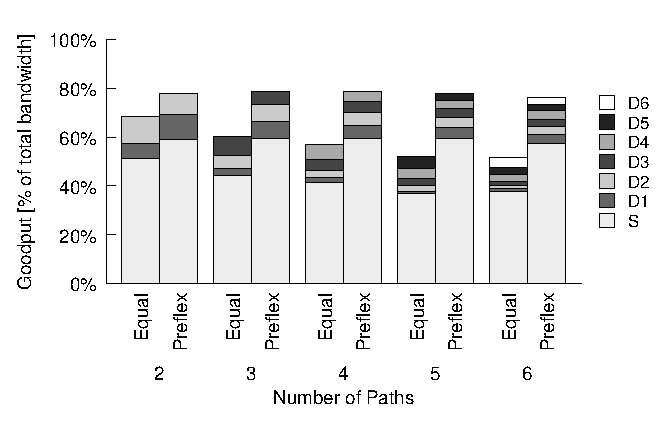
\includegraphics[width=4in]{figures/cate/diffbw}
    \caption{Goodput relative to $B$ achieved by each server for different capacity links.}
    \label{fig:goodputdiff}
\end{figure}

Where bottleneck bandwidth is unequal however equalisation proves inadequate. 
Once again comparing goodput (figure \ref{fig:goodputdiff}) we highlight two significant shortcomings of equalisation which \ac{PREFLEX} overcomes. 
Firstly, goodput for $S$ drops as $N$ increases. 
Unable to realize it is overloading a path, equalisation is reduced to sending traffic over each link at approximately the same rate as the most congested link. 
In contrast, \ac{PREFLEX} detects congestion and adapts accordingly. 
Secondly, the incorrect distribution of traffic due to equalisation in $S$ distorts the goodput of others servers. 
While in \ac{PREFLEX} goodput from $D_{1-N}$ is perfectly balanced, with equalisation traffic crossing the most congested links are directly affected by another domain's inability to distribute its traffic appropriately.
It may seem unfair to judge equalisation for cases where there is a mismatch in link capacity, however this mismatch between link weight and path capacity arises regularly as operators continue to adjust traffic engineering according to local conditions, with little thought spared for the impact this may have further downstream.

\begin{figure}
    \centering
    \includegraphics[width=3.2in]{figures/cate/duration}
    \caption{Mean average flow completion time for equal and differing bottleneck links.}
    \label{fig:duration}
\end{figure}

This impact is in turn perceived by users, who experience longer flow completion times, as shown in figure \ref{fig:duration}. 
In the equal bandwidth case the flow completion time is similar for both balancers.  
Where bandwidth differs however, \ac{PREFLEX} outperforms equalisation and maintains a stable performance when balancing over all six paths.  
This shows that the algorithm scales well as the number of available paths increases. 


\section{Conclusions}
\label{section:malawi:conclusion}

The focus of this work has been on elucidating the main factors that affect flow throughput, but which escape traditional TCP modelling based on end-to-end loss and delay. 
In particular, we explore the changing role of \emph{host limiting}, \emph{application pacing} and \emph{receiver shaping} in defining flow rates across five years of transit traces.
Our results show that for the observed link, over \emph{half} of all inbound TCP traffic can be ascribed to one of the aforementioned constraints.
We show that continuing OS upgrades have progressively lifted the artificial throughput constraints imposed by the host stack. In particular, windowscale negotiation for inbound traffic increased threefold in the observed period, covering over 80\% of all observed bytes by 2012; in addition, we show that buffer sizes have also shown continuing increases over time.

These developments have significantly improved throughput, in particular for smaller flows. However, we also found evidence of throughput limiting effects independent from available end-to-end capacity. This means that no amount of bandwidth will directly improve TCP rates for a considerable amount of traffic.
We show that application-driven techniques for chunked transfer are widely used, accounting for 40\% of all inbound traffic observed in 2011.
%, and that this behaviour is endemic to a wider range of stakeholders than in 2007.
Finally, we uncover evidence of significant receiver traffic shaping prior to 2011 based on the modification of the receiver advertised window in a bid to curtail congestion.
%Uncover evidence of receiver shaping during period of relative contention.



\chapter{A longitudinal analysis of \acs{TCP} traffic}
\label{chapter:malawi}

\renewcommand{\locfolder}{\chapfolder/malawi}
\section{Introduction}

% generic "failures are bad"
Despite being broadly designed for robustness, the current Internet architecture remains remarkably vulnerable to failures.
Managing faults effectively poses a significant operational challenge, in part because faults differ widely in both source and nature, potentially occuring at any layer of the stack and along any element along a path.

% neither is transport
\LOREM
\LOREM

% network methods
Given the commercial nature of the Internet, the onus of providing resilience has instead shifted to network operators.
Traditionally this has been achieved by overloading the routing architecture.
The deployment of real time applications with harder constraints on reliability coupled with better failure detection methods embedded in linecards have provided both the motivation and the means for achieving sub-second recovery within IGP networks \cite{}.
Even with reduced recovery times however, the transient effects of routing changes can still disrupt the forwarding path. 
Under such cases diverse proposals such as Fast Re-Route \cite{}, Loop-Free Alternate next hops \cite{} or Packet Re-cycling \cite{} can provide repair paths for use between the detection of a failure and the convergence of the routing process.

Unfortunately, such methods are rarely sufficient.
Firstly, their application is circumscribed to individual domains, and as such cannot provide end-to-end coverage in a federated, best-effort Internet.
Secondly, there are many faults which do not directly pertain to routing, such as middlebox misconfiguration or hardware malfunctions, and as such go undetected.
Finally, reparation often disregards and potentially disrupts the transport layer by causing out-of-order delivery of packets.

% why now. datacenter, SDN
\LOREM
\LOREM
\LOREM

% layout?
\LOREM
\LOREM


%Outside their networks however, operators are reduced to negotiating service level agreements with their own providers who are invariably unable to cater for such specialized demands \cite{}.
%Even if such terms were met, the Internet architecture provides limited visibility beyond one's own domain.
%This opaqueness, in addition to the fact that failures themselves may be distributed in nature \cite{}, severely limits the ability for a customer network to trace remote problems to a single source \cite{}.
%With no means to hold providers accountable for failures, there is little to enforce the terms of a truly end-to-end SLA.
%
%Unfortunately, such intradomain methods 


%Alongside this increased centralization of resources comes a heightened sense of accountability.
%The commercial nature of the agreements between customers and cloud hosting companies such as AWS \cite{} often involve the establishment of service level agreements.
%Even where such agreements are not explicit, such as the base option of tiered services such as Dropbox or Heroku, there is an inherent need to minimize the impact of outages -- non paying customers may be less demanding, but they are also less sensitive to the switching cost incurred in changing service provider.
%
%Unfortunately, the federated, best-effort nature of the Internet seemingly does not lend itself to such high expectations.



%Under such cases, a network operator is currently expected to detect, repair and recover from such faults.
%Detection often requires scale -- the reliability with which a fault can be identified relies on the proportion of traffic affected. 
%In many cases, faults affecting single flows may go undetected by the network.
%Once detected, reparation varies according to the nature and origin of the fault.
%For some cases, such as intradomain routing, this process is often automated and robust.
%For many others however, such as faulty hardware or misconfigured devices, recovery is difficult and error-prone.
%In either case, the amount of time expended in detection and repair can often preclude recovery, since most flows will terminate after successive timeouts.
%

%Fueled largely by economies of scale in both software management and hardware acquisition and maintenance, the emergence of cloud computing and content distribution networks has lead to a profound shift in Internet traffic.
%
%
%Whereas the advent of broadband connections init
%In contrast to the highly distributed nature of peer-to-peer software which 
%
%
%For one, never has so much been distributed by so few to so many.
%% AS dist graph
%% netflix
%
%\LOREM
%
%% Accountability, resilience

%All intervening equipment is subject to failure along a network path, with recovery time depending not only on \emph{what} happened, but also \emph{where}.
%Within their networks, operators are free to instrument and deploy arbitrarily complex tools to meet requirements. 
%This freedom has lead to a proliferation of proposed improvements in resilience for intradomain settings \cite{}.


%The establishment of SLAs for network availability have traditionally been prefered within the telecom industry in particular, and represent one possible approach to ensuring resilience. An alternative approach is offered by the end-to-end principle. 
%Since end hosts possess both inherent knowledge of application needs and fine-grained measurements on end-to-end path characteristics, the transport layer is often identified as a more natural fit for dealing with fault tolerance at an Internet scale.
%Both SCTP \cite{} and MPTCP \cite{} enable transparent fail-over through multihoming.
%In spite of providing significant features, neither is likely to be widely deployed in the near future: the former lacks critical middlebox support, while the latter is still undergoing standardization.
%Furthermore, the requirement for end-host multihoming has also posed a barrier to deployment.
%Finally, all transport approaches to fail-over confine knowledge of faults within an individual flow: each flow must detect failures independently, even when many flows are affected by the same fault.
%


% Transport is not the answer

% Can we do better with SDN?


%A default forwarding plane, corresponding to the label 0, must be defined and cater for all traffic destinations.
%As with existing routing infrastructure, this single default plane will suffice for most traffic.

%Invariably however, path failures will arise which may affect any number of flows.
%Rather than expecting the network to address end-to-end failures, hosts are allowed to proactively request an overlay plane from the network.





\section{Related work}
\label{section:malawi:related}

Despite their inherent value, longitudinal studies of Internet phenomena are rare. 
Over its short lifespan the Internet has been shaped as much by technological change as by political and commercial realities. 
This dynamic nature does not lend itself to observational studies where data must be collected and curated over long periods of time, and has resulted in a scarcity of relevant datasets. 
What few exceptions exist often stem from collaborative research efforts, such as CAIDA \cite{CAIDA} or Oregon Routeviews \cite{routeviews}. 
The usefulness of these datasets however can be severely affected by the need for data privacy. 
The dissemination of interdomain routing information, where no such requirement exists, has assisted in a wealth of research on wide ranging topics, from quantifying path diversity \cite{Oliveira:2009p203} to locating Internet bottlenecks \cite{Hu:2004p96}. 
In contrast, longitudinal datasets relating to passive measurements have nurtured a much smaller community of researchers often focusing on characterizing traffic \cite{Fontugne:2010p413}. 
Stripped of the locality contained within IP addresses however, researchers are left unable to relate these findings to a wider context.
Instead, cross-sectional studies characterizing traffic aggregated by location are frequently conducted under different contexts \cite{Ager:2011:WCC:2068816.2068870}, but lack the temporal perspective only longitudinal studies can afford. 
Efforts to characterize the spatial properties of traffic over time \cite{Dhamdhere:2011p428,Labovitz:2010:IIT:2043164.1851194,Cho:2008:OSC:1544012.1544024} have defined the changing of Internet topology and traffic alike but fall short of relating such shifts with their impact on relevant metrics such as loss or delay. 

% other work since
This chapter builds on a wealth of prior work on understanding Internet traffic and serves as a reappraisal of significant past contributions.
Flow characteristics and \ac{TCP} behaviour at large are subject to frequent reassessment \cite{Zhang:2002p85}.
Of particular relevance to the current work are passive studies which delve into the inner mechanisms of \ac{TCP}.
In \cite{Jaiswal:2004p242}, Jaiswal et al.\ infer the sender's congestion window by identifying the congestion control variant from the behaviour observed during loss recovery.
The use of separate state machines for each variant however proves unscalable given the many flavours of \ac{TCP} congestion control which have since been deployed.
In \cite{Lan:2006p566}, Lan et al.\ analyse flows according to size, duration, rate and burstiness and characterise the observed correlations for heavy-hitters specifically,
uncovering evidence of increased application influence on flow rates and burstiness and consequently suggest treating flow size and duration as independent dimensions.

One central aspect to the analysis of \ac{TCP} behaviour is the estimation of \ac{RTT} from packet capture data. 
In addition to SYN-based methods, Shakkotai et al.\ \cite{Shakkottai:2004p408} evaluate further techniques to estimate the \ac{RTT} of a unidirectional flow. 
The \textit{rate change} method establishes a relation between the \ac{RTT} and the increase in sending rate, assuming linear window increases during congestion avoidance. 
Unfortunately, this assumption no longer holds, both due to the proliferation of less conservative congestion control algorithms such as CUBIC \cite{Ha:2008p471}, and due to application-driven flow control. 
An alternative is the use of frequency-domain techniques \cite{Veal:2005p412,Lance:2005p565,Qian:2009p429}, which are a natural fit given the self-clocking nature of \ac{TCP}. 
However, a common difficulty with the application of spectral analysis is extracting the fundamental frequency which corresponds to the \ac{RTT} in the presence of noise. 
In applying the Fourier transform to inter-packet arrival times, for example, Qian et al.\ \cite{Qian:2009p429} note that less than half of all flows have distinguishable \textit{flow clocks}; likewise, the \ac{FFT}-based \ac{RTT} recovery was found to be unreliable even after pre-processing available data to enhance inherent periodicities.

% topological influence
Finally, it is important to elucidate what changes in traffic properties are intrinsic to \ac{TCP} and data transfer, and which ones arise from large-scale changes in the \ac{AS}-level topology of the Internet. 
In the decade since publication of \cite{Zhang:2002p85}, the Internet has undergone significant changes, shifting from a broadly hierarchical form to a flatter, more interconnected structure \cite{Labovitz:2010p175,Ager:2012p567}.
Given the longitudinal nature of this chapter and its focus on interdomain traffic in particular, the insights provided by these studies on the macroscopic effects of content consolidation are discernible within the studied dataset, and as such are a source of validation for many of the observations herein.

\section{Dataset}
\label{section:malawi:dataset}

This section provides an overview of the datasets used in this work and some of the data processing required before approaching the longitudinal study of Internet traffic rate limiting. We use the original, unanonymised traffic traces of the MAWI \cite{mawi} dataset, a set of daily traces from the WIDE backbone network which provides connectivity to universities and research institutes in Japan. Traffic is captured daily for 15 minutes starting at 14:00JST. Although this dataset extends back largely uninterrupted from late 2001, we focus on just over five years of data following a network upgrade to the monitored link on October 2006.

The monitored link carries mostly trans-Pacific commodity traffic between WIDE customers and non-Japanese commercial networks. 
We will refer to traffic towards WIDE as \emph{inbound} traffic, whereas traffic originating from within WIDE is referred to as \emph{outbound} traffic.

\begin{table}[!htp]
\scriptsize
\centering
    \begin{tabular}{r|cccccc}
        & & TCP data & \multicolumn{2}{c}{Traffic (TB)} & \multicolumn{2}{c} {Count ($\times10^3$)} \\
        Year & Days & flows (x$10^6$) & In & Out & AS & Prefixes \\
        \hline
        2006 & 91 & 20.52 & 0.43& 0.45 & 10.90 & 56.86\\
        2007 & 350 & 102.56 & 2.11 & 2.49& 17.21 & 113.79\\
        2008 & 358 & 112.26& 2.43 & 2.10& 24.74 & 156.54\\
        2009 & 364 & 113.97& 2.48 & 2.53& 19.71 & 143.87\\
        2010 & 365 & 113.70& 2.58 & 3.43& 20.38 & 148.03\\
        2011 & 358 & 114.74& 3.44 & 5.14& 19.99 & 140.56\\
        \hline
        Total & 1886 & 5777.55 & 13.50 & 16.14 & 34.12 & 341.22\\
    \end{tabular}
    \caption{\label{table:overview}Overview of traced MAWI dataset 
}
  \vspace{-3mm}
\end{table}

A preliminary overview of the dataset used is provided in table \ref{table:overview}. 
In total, 5.7 billion flows containing data are traced over five largely uninterrupted years; this represents approximately 30 terabytes of TCP traffic. For the purposes of this work, we will focus exclusively on inbound traffic, 60\% to 80\% of which originates from port 80, referring only to analysis of outbound traffic when providing a wider context for our findings.
Given the sender side plays a critical role in shaping traffic, analysing traffic for which the source is restricted to a small set of networks within Japan would be of limited use in accurately depicting traffic trends at large.
We instead fix hosts within Japan as sinks, thus sharing a similar perspective on inbound traffic as many other networks. 

\subsection{Tracing TCP Metrics}

All TCP flows are reassembled and analysed for each daily trace.
In addition to the five tuple used to define each connection, we impose two additional restrictions: a contiguous sequence number space and a three minute timeout. These restrictions are helpful to deal with port reuse and unterminated flows respectively.  
Although the total number of TCP flows increased dramatically in 2011, the number of flows \emph{for which data payload was seen} has remained stable, averaging over 100 million data flows traced per year.  

There is much prior work with regards to reconstructing TCP flow from passive measurements and using this information to understand the end-to-end properties of traffic \cite{firstRTT,Jaiswal:2007p233,Rewaskar:2007p195,Shakkottai:2004p408}. However, the MAWI traces impose two constraints which require careful consideration, and ultimately led to the use of a custom TCP tracer. 
The first one is the proportion of bidirectional flows, that is flows, where both forward and reverse path are seen. 
In the dataset used this fluctuates between 40\% and 60\% over five years.
Most available TCP tracers either ignore or are inadequate at processing unidirectional flows. 
The second one is the short duration of each individual trace file. 
At only 15 minutes of line-rate data capture per day, it is wasteful to ignore flows which are not complete. Although the number of flows for which a SYN and FIN in either direction is observed has remained consistently high until late 2011, these flows are normally \emph{mice}, i.e. flows that tend to be brief and which carry little traffic individually. In contrast, most \emph{elephants} (flows that carry significant traffic individually) have durations that exceed that of each trace file. 

%rtts traced
%While many metrics are extracted for each flow, for the purposes of this paper we will focus only on detailing how we collected delay and loss.
%Passive RTT estimates, calculated as the offset between a data packet and its respective acknowledgement, require both directions to be observed at the measurement point. 
%This provides delay estimates between the measurement point and the receiver, as illustrated in figure \ref{fig:synrtts}. 
%For flows where data is transfered in both directions, we will obtain in effect two separate estimates, $RTT_{m2a}$ and $RTT_{m2b}$, illustrated in figure \ref{fig:synrtts}. 
%Together they form the total end-to-end delay experienced by end-hosts. 
%For the remainder of this paper, the term RTT will refer to delay between our measurement and destinations outside WIDE. 
%We discard the delay between measurement point and hosts within WIDE for two reasons. 
%It is both negligible for a large proportion of traffic, which is highly concentrated within the Tokyo metropolitan regions and immediate surroundings, and extremely large for a very small subset of hosts located outside Japan, as WIDE has in the past acted as a provider to academic institutions in Indonesia through a satelite uplink. 
%By decoupling both directions we focus purely on the changes in delay to locations outside Japan. 
%This incurs a reduction in the range of destinations for which we can obtain estimates - only bidirectional traffic can be traced this way. 
%For the set of destinations we will study in this paper, we shall show that this reduction is small. 
%For tracking delay changes for unidirectional traffic for other purposes, MALAWI includes RTT estimates extracted from the SYN exchange.

Loss is inferred by accounting for \emph{retransmissions} in the upstream data and \emph{out-of-order packets} in downstream data; for the remainder of the paper we will refer to the \emph{end-to-end loss} as the sum of out of order and retransmitted data bytes over the total data bytes in a given direction.
% XXX: remove RTT ref?
%Tracking both retransmissions and out-of-order packets accurately requires a reliable RTT estimate, which can only be obtained for bidirectional flows. We forfeit some precision by not taking this into account, as we wish to be consistent in how we estimate both metrics independently of the type of flow and aggregation. 
Pragmatically, we found this to be an adequate indicator of loss --- with the exception of \emph{hanging} TCP connections. 
In these cases where connectivity is lost, a host will proceed to retransmit packets while performing an exponential backoff. 
Although this results in negligible overall traffic, it can significantly skew the inferred loss ratio for uncommon destinations for which little traffic exists. 
To account for these cases, we imposed a 3-second timeout on retransmissions after which we consider the congestion feedback loop to be broken. 

Each daily trace in the dataset is processed from a packet level capture into a collection of flow level statistics. 
This gives us insight into the end-to-end characteristics of traffic. However, since a core objective of this work is to augment this time-based information with data describing the endpoints of each flow, aggregating by location is also required. 

\subsection{Aggregating by Location}

Location information is added by mapping the original source and destination IP addresses to its geographical and topological counterpoints. 
We use the \emph{routeviews} archives to reconstruct the mapping between each IP and both AS and network prefix; bi-hourly dumps of BGP RIBs are available in the WIDE archives since mid 2003. 
We reconstruct a daily RIB based on the views provided by contributing ASes, in particular IIJ and APNIC. 
Since exact routes are not disclosed (there is no record of local policy), we have no knowledge of the route taken by packets; this of course does not hinder our ability to consistently map IPs to ASes. While discrepancies in AS destinations exist between different routeviews contributors, we note that this happens almost exclusively on prefixes for which no actual traffic is seen. 

Mapping IP to country is done through the use of GeoLite \cite{maxmind}, a commercial geolocation database. 
While the accuracy of this solution is often disputed, we are not overly concerned with locating traffic at a fine granularity. 
We will mostly focus on tracking traffic by country and, for larger countries such as the U.S, by region, in order to capture shifts over time.
GeoLite proves adequate on both counts.
The archive for geolocation data only extends to 2009, before which we must rely on the earliest match. 
Additionally, we verify if the destination or source AS have maintained the same administrative mapping up until mid 2009 in the relevant RIR (regional internet registry) archives; otherwise, we do not associate a flow to a geographical location.
% bridging paragraphs to save space.
After associating flows to country, region, AS and network prefix for both source and destination IPs, we aggregate flow statistics over each location identifier. 
This generates a daily collection of location identifiers and associated flow properties, from which we can sketch the geographic and topological properties of the dataset over time.

\section{Methodology}

Providing a macroscopic view on where traffic originates from, and in what quantity, can be achieved by simply binning packets into flows and accumulating byte counts over geographical or topological locations. 
Uncovering application layer characteristics (i.e. \textit{how} traffic is sent) is a more complex problem that requires additional methods to reverse engineer transport behaviour.
The aim of this section is to describe a process which distinguishes those flows which have their throughput limited by mechanisms other than the usual \ac{TCP} response to loss and delay.
Each flow can be characterized as being either application paced, in which the sending application is limiting the data provided, host limited, whereby local constraints at either end host cap throughput, or receiver shaped, in which an artificial constraint is imposed by either a middlebox or receiver.

The classification proceeds in stages. 
Before classification, it is necessary to reconstruct the RTT of the flow if the flow is not bidirectional.  
This is achieved in section \ref{subsection:malawi:PeriodicEnhancement}. 
Because the sender's TCP state machine cannot be directly observed it is necessary then to estimate the size of the congestion window by observing the number of unacknowledged bytes in flight (\textit{flight size}).
This reconstruction is described in section \ref{subsection:malawi:flightAggregation} and provides the basis for flow classification. 
Flows are then checked in turn to see if they are application paced, host limited or receiver shaped and classified as belonging to the first of these classes for which they fulfill the necessary conditions.
Flows in none of these classes are either limited only by the network (delay or loss conditions) or are insufficiently large to trigger any further constraints.

\subsection{RTT Estimation}
\label{subsection:malawi:PeriodicEnhancement}

Building on prior work presented in section \ref{section:malawi:related}, this section proposes an algorithm that scalably recovers the RTT from one-directional traffic traces. 
% XXX: below implies microflights were used, but these aren't described (remove as appropriate)
Although \ac{RTT} estimation is a difficult problem, simplifying assumptions can be made.
For the \ac{MAWI} dataset most \acp{RTT} are relatively large, with the closest neighbouring country, South Korea, roughly 40ms away.
By only processing bidirectional traffic from Japan, the expected \ac{RTT} range can be reduced for all other traffic.
The recovery mechanism then enhances the natural periodicity of traces and scalably constructs flights associated with specific application and protocol behaviour.
In the following the mechanisms required by these two goals are described. 
%
% Why does this work?
%
In normal operation, many \ac{TCP} operations involve request-response cycles between two endpoints in which the \ac{RTT} $T$ provides a natural \emph{clock}.
Hence, the most natural way to estimate \ac{RTT} from \ac{TCP} traces is to correlate requests and responses exchanged in both directions. 
If only one direction of data is observed however, $T$ cannot be directly observed. 
Instead, it must be estimated from the way in which \ac{TCP} packets cluster in time due to the batching of request-response operations.

The \ac{TCP} \ac{cwnd} determines the number of unacknowledged bytes that a \ac{TCP} flow may maintain at any point in time. 
This can be referred to as \emph{bytes in flight} because they are in transit between the sender $S$ and the receiver $R$; an equivalent definition applies for the number of \emph{packets in flight}. 
Once $S$ has transmitted \ac{cwnd} data bytes, it will refrain from transmitting more until either some bytes are acknowledged by $R$ or \ac{cwnd} is increased by the sender. 
In the absence of losses, neither of these events can happen until a \ac{TCP} \ac{ACK} is received; this immediately reduces the number of unacknowledged bytes, but may also lead to a significant \ac{cwnd} increase (during e.g. \emph{slow start}). 
% XXX: number of unacknowledged bytes reduced, or CWND?
In the presence of losses, however, bytes can be re-sent if a packet is timed out and considered lost; in this case, the number of unacknowledged bytes is reduced.

%
% What is our main contribution, algorithmically speaking?
%
The main difficulty associated with one-sided TCP flow reconstruction is as follows.
Let $t_1, t_2, \ldots$ be a set of times at which packets $p_1, p_2, \ldots$ were observed at $S$ en route to $R$.
Suppose that a packet $p_j$ of size $b$ is observed at time $t_j$.
In addition, suppose that approximately one RTT $T$ later, the sender $S$ receives an ACK $a_j$ from $R$ for the $b$ bytes of $p_j$.
At this point, the TCP stack in $S$ will decrease the number of unacknowledged bytes by $b$, thus opening the possibility for sending additional traffic to $R$.
This can lead to another packet $p_k$ to be transmitted; let this packet be observed at time $t_k$ as it is sent towards $R$.
Assuming that processing delay is insignificant, the RTT experienced by $p_j$ can be approximated as $T \approx t_k - t_j$.
Now consider what happens if packets are only observed in the $S \rightarrow R$ direction.
Under such conditions, it is not possible to ascertain whether $p_k$ was sent explicitly as a result of $S$ receiving the unobserved \ac{ACK} $a_j$, or whether it was sent as a result of an \ac{ACK} $a_i$ associated with a previous packet $p_i$ rather than with $p_j$.
If, however, a packet $p_l$ is eventually observed that did result from the reception of $a_j$, the \ac{RTT} can be estimated as $T \approx t_l - t_j$ with $t_l > t_k$.
Following this same reasoning, approximately one \ac{RTT} later a packet $p_m$ will be observed for which $2T \approx t_m - t_j$; this can potentially continue for as long $S$ has data to send and $R$ continues sending \acp{ACK}.
This is the underlying reason that \ac{RTT}-related periodic regularities arise when considering the timestamps of observed packets \cite{Qian:2009p429}.

The reasoning above is at the heart of the proposed algorithm to improve \ac{RTT} recovery by enhancing packet stream periodicity. 
Assume that a packet $p_j$ is observed at time $t_j$. 
Considering the set $\mathcal{T}_j$ of all values of $\Delta t = t_k - t_j$ for every $k > j$, it is apparent that it will include estimates not only for the \ac{RTT} $T$, but also for all its multiples $2T, 3T, \ldots$ 
If $t_l-t_k \approx T$ and $t_k - t_j \approx T$ then it follows that $t_l - t_j = 2T$, and this value will also be included in $\mathcal{T}_j$. 

By maintaining a set $\mathcal{T}_j$ for every packet $p_j$ observed, at least some of its values will correspond to estimations of multiples of the \ac{RTT}. 
It then follows that by creating a set $\mathcal{T}$ that includes values calculated starting from every packet $p_j$ so that $\mathcal{T} = \cup_j \mathcal{T}_j$, numerous estimates for $2T, 3T, \ldots$ will also be included. 
Hence, the probability density function $H(t)$ of the values in $\mathcal{T}$ should show peaks around multiples of the \ac{RTT} (see Figure \ref{fig:histogram}). 

\begin{figure}
  \centering
  \includegraphics[width=0.8\textwidth]{figures/malawi/rttbin.pdf}
  \caption{$H(t)$ for flow displayed in Figure \ref{fig:hostlimited}. The horizontal line delimits $\overline{H}$ while the highlighted bin denotes the bidirectional RTT estimate.\label{fig:histogram}}
\end{figure}

%
% Explain why did we use FFT
%
The algorithmic recovery of $T$ from $H(t)$ presents additional challenges. 
In particular, $H(t)$ may include a large number of \ac{RTT} multiples, and a peak will be found for all of them. 
Crucially, all these peaks may be of comparable magnitude, complicating the task of selecting a single peak.
Moreover, these peaks need not be very pronounced, with histogram bins in close proximity of the peaks have very similar values as the peak itself. 
As such, taking \ac{RTT} candidates directly from $H(t)$ may result in a large set of similarly-valued bins situated around a peaks at multiples of the \ac{RTT}. 

Three recovery algorithms for $T$ are attempted.
First, as a baseline, the highest peak in $H(t)$ is selected as a candidate for $T$. 
In addition, expanding upon the work of Qian et. al. \cite{Qian:2009p429} a frequency-domain representation of $H(t)$ is used to identify $T$. 
This is done by selecting the highest peak of $|\hat{H}(\omega)|^2$, the \emph{energy spectral density} of $H(t)$ (i.e. the norm squared of the Fourier transform of $H(t)$). 
Finally, a custom utility-based technique that operates directly on $H(t)$ is proposed which achieves superior performance to both of the aforementioned methods.

%\subsubsection{FFT-Based RTT Recovery}
%We extract periodicity information from $H(t)$ by looking at $\hat{H}(\omega)$, the \emph{energy spectral density} of $H(t)$. Formally, $\hat{H}(\omega)$ is defined as the norm squared of the Fourier transform of $H(t)$, so that $\hat{H}(\omega) = |\mathcal{F}(H(t))|^2$. Using $\hat{H}(\omega)$ markedly improves the quality of our RTT estimation because the frequency peak corresponding to the RTT usually accounts for a much larger proportion of the total frequency domain energy than other peaks in $\hat{H}(\omega)$, leading to a much simpler discrimination of the true RTT. However, due to RTT changing during the lifetime of a flow, and also due to the expected noise associated with real-life data sources, $\hat{H}(\omega)$ can also occasionally include large peaks at frequencies unrelated to the RTT. In order to filter these out, we take a set of 10 frequency candidates from $\hat{H}(\omega)$, and use their associated periods as RTT candidates in our flow reconstruction algorithm (see Section \ref{
%subsection:malawi:flightAggregation}). We then select that RTT candidate which exhibits the smallest error, that is, that one which yields closest agreement with observed data.

%
% Algorithmic hacks
%
%To streamline our algorithm for streaming use, we use the following heuristics and approximations. Firstly, we define a range $[T_{\min}, T_{\max}]$ representing the range over which we find the RTT values of interest. Then, for each packet $p_j$, we build a subset $\mathcal{T}_j'$ of $\mathcal{T}_j$ by including all values of $t_j - t_k < T_{\max}$. We then generate $\mathcal{T}' = \cup_j \mathcal{T}_j'$ and approximate $H(t)$ by considering a histogram of the values in $\mathcal{T}'$. As usual, we do this by counting the frequency with which its values are observed in the ranges $[0,\tau)$, $[\tau, 2\tau)$, $[2\tau, 3\tau), \ldots$ where $\tau$ is the time resolution required. 


\subsubsection{Utility-Based RTT Recovery}
\label{sect:utilityBasedRecovery}

This method relies not on the identification of periodicities, but on explicitly matching experimentally found signatures. 
To this end, we consider the peaks of $H(t)$, which are then considered RTT candidates.  
However, trivial discriminators (such as simply selecting the highest peak) are not reliable. 
In this case, it was found experimentally that repeatable peaks and troughs also occur at multiples and sub-multiples of $T$, with the most important ones being $\frac{T}{3}$, $\frac{T}{2}$, $T$ and $2T$. 
We design this detection algorithm around the idea that a given pattern of peaks and troughs can identify $T$.

If we define $\overline{H}$ as the mean height of $H(t)$, we can define a per-peak utility function $p(t)$ so that 
\begin{equation*}
p(t) = 1.0 - \exp\left(-2.0 \left(\frac{H(t)}{\overline{H}}\right)\right) \mbox{.}
\end{equation*}
This function has several advantageous properties: it is 0 if $H(t)$ is zero, 1
if $H(t)$ is infinite, and $0.5$ if $H(t) = \overline{H}$.  In other
words it is a measure of the \emph{peakiness} of the data, with $p=1$ identifying
an infinitely high peak, $p=0$ identifying an empty histogram bin (trough), and $p=\frac{1}{2}$ 
implying that $H(t)$ is of exactly average height at that point. We can then score each candidate using the following utility function:
$$
P(t) = 1.5 p(t) + p(2t) - p\left(\frac{t}{2}\right) - p\left(\frac{t}{3}\right).
$$
That is, the candidate RTT $t$ scores highly if it is itself a peak, if it has a peak
at a multiple $2t$, and if it also manifests troughs at submultiples $\frac{T}{2}$ and $\frac{T}{3}$.
The factor of 1.5 was added after observations
showed that the peak at $T$ was the most important factor in determining
whether a candidate was the true RTT. Similarly, additional multiples and submultiples 
were excluded as they showed very limited discriminating power experimentally.

\begin{figure}
  \centering
  \includegraphics[width=0.8\textwidth]{figures/malawi/rttcomp.pdf}
  \caption{Accuracy of RTT estimator when compared to the median value of bidirectional estimate.}
\end{figure}

\subsubsection{Comparing RTT Recovery Algorithms}
\label{sect:comparingRecoveryAlgos}
As described in Section \ref{subsection:malawi:PeriodicEnhancement}, $H(t)$ is calculated in such a way that RTT periodicity is amplified. 
This means that FFT-based techniques could potentially perform better on $H(t)$ than on the packet stream with no pre-processing. 
However, this is complicated not only because $H(t)$ contains periodicities at multiples of $T$, but also discontinuities that generate harmonics at frequency multiples of the RTT fundamental. 
Hence, although the FFT $|\hat{H}(\omega)|$ of $H(t)$ is much cleaner than that of the packet interarrival time series on its own, its maximum peak rarely coincides exactly with the RTT clock (this corroborates reports by Qian et al \cite{Qian:2009p429}). 
Thus, applying the FFT leads to another \emph{peak detection problem} in which the RTT fundamental needs to be extricated from its harmonics and sub-harmonics. 
The trivial solution to this problem, the application of a bandpass filter around the RTT frequency, is of course unfeasible because the bandwidth and 
centring of such a filter depend on the RTT which is itself unknown.
The utility-based algorithm described in Section \ref{sect:utilityBasedRecovery} can hence be applied in either the time domain or the frequency domain; we chose to do it on the former on the interest of expediency and lower computational cost.

\newcommand{\RTTHeader}{Below & Above}
\newcommand{\SmallFlowName}{\textless 10MB}
\newcommand{\LargeFlowName}{\textgreater 10MB} 
\begin{table}
\footnotesize
\centering
\begin{tabular}{ p{1.5cm} p{1.2cm} p{0cm} p{.6cm}p{.6cm} p{0cm} p{.6cm}p{.6cm}}
& & & \multicolumn{2}{c}{Peak} & & \multicolumn{2}{c}{Utility-based} \\
\cline{4-5} \cline{7-8}
& Flow size & & \RTTHeader & & \RTTHeader \\
\cline{4-5} \cline{7-8} 
\multirow{2}{*}{Receiver side}  & \SmallFlowName && 4.31 & 9.13 && 4.58 & 6.35
\\ 
                                & \LargeFlowName && 6.72 & 6.43 & 4.97 & 5.33
\\
\multirow{2}{*}{Sender side}    & \SmallFlowName && 2.94 & 8.37 && 3.29 & 4.80
\\
                                & \LargeFlowName && 6.41 & 9.06 && 5.40 & 11.06
\\
\end{tabular}
\caption{\label{table:rttRecovery}Performance of RTT recovery algorithms}
\vspace{-3mm}
\end{table}

The performance of the analysed RTT recovery mechanisms is presented in Table \ref{table:rttRecovery}, that shows the percentage of total flows below and above the RTT range given by the bidirectional estimates.
We separate things for \emph{inbound} traffic (where we are positioned at the receiver side) and \emph{outbound} traffic (where we are positioned at the sender side). The utility-based algorithm is particularly useful to address RTT underestimation for flows over 10MB in size, which is our main objective since precisely that kind of estimation error would interfere with our ability to correctly decouple application behaviour from RTT-scale dynamics.


%For the most part, the utility based method improves on underestimation, which is our main objective since that would interfere with our flight reconstruction (i.e. generate lots of gaps).
%The exception (kind of) is traffic from the sender side, which in our training set (one week per year), had quite a lot of host limited traffic (paced out, no signal to recover).
%In this case, not a problem, since if the flow is long enough multiples of the RTT will still reveal host limitation, but will give us a smaller window..


\subsection{Flow Classification}
\label{subsection:malawi:flightAggregation}

One fundamental precondition to decouple the influence that network loss, host configuration and TCP behaviour has on the throughput experienced by a flow is the reconstruction of the congestion window behaviour of TCP flows on the basis of observed data. 
Unfortunately, the congestion window value is internal to the sender's TCP state machine and may not manifest itself in the absence of sufficient data from the application layer. 
A more easily observed quantity which serves as a reasonable proxy for the congestion window is the number of unacknowledged bytes in flight, henceforth referred to as the \textit{flight size}, which can be derived given an accurate estimate of the end-to-end delay.
The evolution of both flight size and RTT can in turn be used to ascertain to what extent throughput is regulated by limitations imposed at different layers of the networking stack.

% definitions
Given a candidate RTT, we can aggregate a stream of packets with arrival times $t_1, t_2, \ldots$ into a stream of \emph{flights}. 
Intuitively, a flight is a clustered subset of a TCP flow which exhibits its own temporal coherence; alternatively, it can be though of as a series of consecutive packets that were (roughly) generated by the sender as a response to the same protocol operation. 
A flight $f_i$ that begins
with the $j$th packet and ends with the $k$th is defined to have a \emph{total flight time} $\tau_i = t_{k+1} - t_j$. 
The algorithmic selection of initial and final packets in such a way that the resulting flights are indicative of TCP behaviour remains an open problem. 
Since we assume that the RTT provides a natural time frame for the operations of TCP, in the algorithm presented in this work, given an initial packet $\pi_j$ and an RTT estimate $T$, the $k$th (and final) packet is selected to minimise \emph{the flight time error} $e_i = |T - \tau_i|$. 
This mechanism follows closely the methodology described in \cite{Zhang:2002p85}, with the exception that we do not attempt to define flights as being both adjacent and disjoint; rather, we decompose flows into a stream of potentially overlapping flights. 
This helps the algorithm mitigate the deleterious effects of small deviations in the estimated RTT, which alters the properties of each flight. 
Furthermore, since the flight size is continuous in time, it makes little sense to restrict ourselves to a single sample per round trip time.

Having obtained flight information from each flow, we next consider what is the predominant factor that affects its throughput. 
Within the context of TCP, we classify flows as being artificially constrained by three distinct processes: \emph{application pacing}, \emph{host limited} and \emph{receiver shaping}.

\begin{figure}
\centering
  \centering
  \begin{subfigure}{1.0\linewidth}
    \includegraphics[width=1.0\textwidth]{figures/malawi/youtube.pdf}
    \caption{Application paced. \label{fig:youtube}}
  \end{subfigure}\\
  \begin{subfigure}{1.0\linewidth}
    \includegraphics[width=1.0\textwidth]{figures/malawi/hostflow.pdf}
    \caption{Partially host limited. \label{fig:hostlimited}}
  \end{subfigure}\\
  \begin{subfigure}{1.0\linewidth}
    \includegraphics[width=1.0\textwidth]{figures/malawi/awnd.pdf}
    \caption{Receiver shaped. \label{fig:awnd}}
  \end{subfigure}
  \caption{Flight size over time for flows affected by different artificial constraints. \label{fig:kindsOfFlowEffect}}
\end{figure}


\subsubsection{Application Paced Flows}
\label{sssec:app}

A flow whose throughput decreases because it has no outstanding data to send is temporarily limited by the application. 
Flights can be identified as being \emph{application limited} if terminated with a packet smaller than the maximum segment size (MSS) and followed by an inter-arrival time greater than the RTT, as consistent with \cite{Zhang:2002p85}. 
The underlying reason for this defintion is that most TCP implementations will wait some time for subsequent bytes to be written to the socket if the next packet to be sent is smaller than the MSS, unless the TCP\_NODELAY option is set \cite{nagle1984rfc}.

A flow with \emph{application limited} flights however is not necessarily \emph{application paced}. In practice, all flows for which the final packet is observed contain at least one such flight.
For the purposes of our work, we are focused on identifying cases in which throughput is predominantly determined by application behaviour.
One such example is illustrated in figure \ref{fig:youtube}, in which a stream is delivered by periodically writing blocks to the sending socket.
The resulting network-level behaviour is distinct from traditional congestion control: short bursts are interspersed with protracted silence.
Application limited flights, which terminate on non-MSS packets, are highlighted at the end of each burst.

This behaviour is in stark contrast to that exhibited in figure \ref{fig:hostlimited}, where distinct transfers are multiplexed on top of a single transport association over time.
From the perspective of the network, there is little to distinguish the behaviour of such traffic from independent TCP flows.
Application paced connections such as Youtube traffic however exhibit a degree of regularity which can potentially be exploited by the network in predicting demand or smoothing bursts.

In order to identify such recurring behaviour, we identify flows as being \emph{application paced} if the period between bursts terminated by \emph{application limited flights} is consistently under 10 seconds and the standard deviation of the intermediate pauses is under one second.
This definition in particular purposely ignores flows which exhibit long silence periods due to user interaction, and follows closely the behaviour historically associated to Youtube streaming in particular.

\subsubsection{Host Limited Flows}
\label{sssec:host}

Given sufficient bandwidth and traffic to send, a flow may encounter local constraints at either end-host which cap its throughput. 
For instance, the buffer space allocated on both the sender and receiver side is often pre-configured, and it is common practice to tune these values down on popular servers and managed infrastructure in a bid to conserve memory or bandwidth.
A receiver is also limited in the window size it can announce to the remote sender; if the windowscale option \cite{jacobson1992tcp} is not negotiated during the TCP handshake, the advertised window cannot exceed 64KB.

In both cases, a local decision by either host can determine the upper bound of the flow rate.
These \emph{host limited} cases are characterised by a constant window size over time.
The methodology described for flight aggregation at the beginning of this section typically generates a large number of flights, representing many likely combinations given a base RTT estimate.
In order to identify the flat-lined behaviour of a host limited flow, we first filter the flight stream to remove some of the uncertainty derived from small fluctuations in the RTT.
We then select the maximum flight size observed for each RTT interval, and declare a sequence of flights to be host limited if the same maximum was observed over six consecutive RTTs (this is twice the period suggested in \cite{Zhang:2002p85}).
In practice, increasing the period over which the maximum window size is tracked allows us to more accurately discern between host limited behaviour and more conservative bandwidth probing, such as that performed during the convex phase of TCP CUBIC \cite{Ha:2008p471}.

A flow may be host limited for only brief periods of its lifetime, as illustrated in figure \ref{fig:hostlimited}.
To filter out such cases where host limitations are not the predominant factor in defining flow throughput, we further enforce that in addition to host-limited flights, the average window size must over a flow lifetime should be within 10\% of the inferred host limit, which is not the case in figure \ref{fig:hostlimited}.

In practice, flows can exhibit both application pacing and host limitations, with bursts being sent at a capped window size followed by application pauses.
In such cases, a flow will still be classified as being \emph{application paced} if it meets the requirements set out in the previous section, as doing so provides evidence that it controls throughput in spite of the degraded performance provided further down the stack. 
This line of reasoning applies equally to the occurrence of sporadic loss; so long as block delivery is ensured within the timeframe dictated by the application, it remains in control.

\subsubsection{Receiver Shaped Flows}
\label{sssec:rec}

A flow which is neither \emph{application paced} or \emph{host limited} can still be artificially constrained by flow control (rather than by congestion control).
Traditionally, in TCP the sender is responsible for regulating throughput. 
However, the receiver can also shape throughput by manipulating the \emph{advertised window} announced on every acknowledgement.
Such receiver-window auto-tuning has been available on Windows operating systems since Vista \cite{vistaReceiveWindow}, and can also be leveraged by middleboxes in order to throttle inbound traffic \cite{appEx}.

In order to evaluate the potential impact of such behaviour, we further propose a heuristic to identify receiver-shaped traffic.
For flows in which both directions of traffic are observed it is possible to correlate the evolution of the advertised window with the size of reconstructed flights.
Figure \ref{fig:awnd} displays an example of a receiver-shaped connection, in this case throttled by an intermediate middlebox.
Since the advertised window may be fluctuating, it is not always obvious which of the many updates were effectively applied by the sender as successive values supersede each other.
An example of a reconstructed flow which is subjected to receiver shaping is displayed in Figure \ref{fig:awnd}.

For flows in which both directions are observed, it is possible to classify flights as being receiver-shaped if there is a statistically significant correlation between the advertised window size and the maximum flight size observed.
Harnessing the stream filtering used in detecting host limited behaviour, we perform such analysis over a sliding window of 10 RTT intervals.
A flight is flagged as being receiver shaped if the correlation between receiver window and flight size is statistically significant; a flow is considered to be predominantly receiver shaped if over half of its flights are flagged as such.
We do not perform this covariance analysis on flights which contain out-of-order or retransmitted packets. 
In these cases, both the receiver and sender window sizes are correlated \emph{by definition}. 
In the former case, the receiver buffer will temporarily fill expecting the next packet in sequence, in the latter case, TCP will reduce its window.

Given that receiver shaping classification requires correlating information in both directions of a TCP connection, it will come as no surprise that the absence of the reverse path can introduce false positives into our measurements. 
This happens because any given flow might be receiver shaped in such a manner that the heuristic erroneously attributes its behaviour to host limitations. 
In the absence of additional evidence, this misclassification is difficult to detect explicitly. 
Instead, we calculate the ratio of receiver shaped flows which would have been incorrectly identified if the reverse path were not observed. 
This error rate can then be used to evaluate the accuracy of classifier results.

\section{Performance Analysis}
%4.1) Balancing between two paths with high loss using fixed time unit
% using only loss-based balance in a simple regime where that works.
% Show how this converges quickly when one path suddenly gains
% background traffic (and hence loss).
%4.2) Balance between several paths with high loss and fixed time unit
% in simple regime where that works.
%4.3) Introduce experiment where equi-path is needed for probing and
% conservative is needed for low loss regime.
%4.4) Introduce experiment where time-scale tuning is needed to get
% good assessment of loss in low traffic regime.

We evaluate \ac{PREFLEX} through simulation in ns-3 \cite{ns3}. 
Since \ac{PREFLEX} balances traffic using loss rather than load, there is a need to emulate the end-to-end behaviour of traffic. 
This proves more challenging than analysis of existing traffic engineering proposals which typically only focus on adjusting load, since we wish to verify the impact of \ac{PREFLEX} on end-user metrics. 

\subsection{Methodology}
\label{section:methodology}

For all simulations we will use the topology displayed in figure \ref{fig:topo}. 
The topology links a client domain $C$ to a server domain $S$ through $N$ paths with equal bottlenecks $L_i$, and total bandwidth $B=\sum{L_i}$. 
While a domain is represented as a single entity in figure \ref{fig:topo}, each domain is composed by a traffic generator connected to a router. 
Client $C$ generates $G$ simultaneous \ac{HTTP}-like requests (or ``gets") from $S$ according to a specified distribution, described at the end of this section. 
As traffic flows from $S$ to $C$, the router within $S$ is responsible for balancing traffic over all available paths.

\begin{figure}
    \centering
    \includegraphics[width=2.5in]{figures/cate/topo}
    \caption{Simulation topology}
    \label{fig:topo}
\end{figure}

Across simulations, as the number of paths increases, total bandwidth $B$ and the number of simultaneous requests $G$ is fixed. 
In this manner we wish to analyze how \ac{PREFLEX} balances traffic as the granularity with which it can split traffic becomes coarser.

Since we are interested in evaluating how \ac{PREFLEX} shifts traffic in response to loss, we introduce additional ``dummy" servers $D_i$ which are connected to $C$ through a single path. 
We partition the total simulation time $T$ into $N+2$ intervals starting on $s_i$, in which $s_0$ and $s_{N+1}$ have no traffic to $D_i$. 
Starting at time $s_i$, client $C$ generates $g_i$ requests to $D_i$ according to the same distribution as used to server $S$. 
All requests to $D_i$ end at time $s_{N+1}$. 
Equation \eqref{eq:si} sets the start time $s_i$ for requests to $D_i$ as a function of total simulation time $T$ and number of paths $N$. 
Likewise, equation \eqref{eq:gi} sets the number of simultaneous requests $g_i$ to $D_i$ as a function of $G$, the total number of requests to $S$, and $N$.
\begin{equation}
s_i = T\frac{i}{N+2}
\label{eq:si}
\end{equation}
\begin{equation}
\theta_i = \frac{\frac{1}{N+1-i}}{\sum{\frac{1}{N+1-i}}},  g_i = G\theta_i.
\label{eq:gi}
\end{equation}

Figure \ref{fig:demand} illustrates the number of simultaneous gets from $C$ to $D_i$ for $N=2$ (used in the example shown in figure \ref{fig:two}) and $N=4$. 
Generating cross-traffic in this manner serves two purposes. 
Firstly, $\sum{g_i}=G$, so independently of the number of concurrent paths, the maximum load in the system is $2G$. 
However, as the number of paths increases, the fluctuation in load for each path becomes smaller, and so we will stress the sensitivity with which \ac{PREFLEX} balances traffic. 
Secondly, the number of requests for each $D_i$ over time is the same. 
Over timescale $T$, equalisation appears to be an acceptable strategy, however within each interval we will show it performs poorly achieve consistent behaviour. 
This is a fundamental limitation of offline traffic engineering, which is calculated over very long timescales and is unable to adapt as traffic routinely shifts.


\begin{figure}
    \begin{subfigure}[b]{.5\linewidth}
        \centering
        \includegraphics[width=2.25in]{figures/cate/dummy2-crop.pdf}
        \caption{$N=2$}\label{fig:1a}
    \end{subfigure}%
    \begin{subfigure}[b]{.5\linewidth}
        \centering
        \includegraphics[width=2.25in]{figures/cate/dummy4-crop.pdf}
        \caption{$N=4$}\label{fig:1b}
    \end{subfigure}
    \caption{Number of requests from $C$ to cross traffic servers $D_i$ for different values of $N$}
    \label{fig:demand}
\end{figure}

We now specify the settings common to all simulations, including those previously shown in figure \ref{fig:two}. 
Total simulation time $T$ is set to $1200$ seconds, while total bandwidth $B$ is fixed at $240$Mbps. 
The number of requests $G$ sent from $C$ to $S$ is set to 240. 
Upon completing, a request is respawned after an idle period following an exponential distribution with a $15$s mean. 
Transfer size follows a Weibull distribution with an average value of $2$MB. 
These values attempt to reflect traffic to a single prefix with a file size that mimics the small but bursty nature of web traffic, which does not lend itself to being balanced by the end-host. 
\ac{PREFLEX} is configured with $\beta_E = 0.05$, $\mu_{min}=0.01/N$ and $\delta=0.005$.

\subsection{Varying bottleneck distribution}

We start by examining the case where all bottlenecks share the same bandwidth, $L_i=B/N$, and compare \ac{PREFLEX} to equalisation, which mimics traffic engineering techniques based on hashing flow tuples and assigning them to a path. 
The goodput, calculated as the total data transfered to client $C$ by flows completed within $T$, is shown for both equalisation and \ac{PREFLEX} methods in figure \ref{fig:goodputeq}. 
While both saturate most available bandwidth, equalisation leads to disproportionate distribution of goodput amongst competing traffic. 
As loss is not equalised over all paths, the amount of goodput achieved by servers $D_i$ differs despite demand being similar.

Equalisation, even when weighted according to local link capacity, is often prone to remote bottlenecks. 
We investigate the effect of differing bottlenecks by repeating previous simulations with the same total bandwidth $B$, but with $L_i$ set proportionally to $B$ in a similar manner to \eqref{eq:gi}, that is $L_i = \theta_i B$.


\begin{figure}
    \centering
    \includegraphics[width=4in]{figures/cate/eqbw}
    \caption{Goodput relative to $B$ achieved by each server for equal capacity links.}
    \label{fig:goodputeq}
\end{figure}

Figure \ref{fig:goodputeq} shows the goodput as a proportion of total link bandwidth for the case where all links have equal bandwidth. 
We vary the number of links $N$, and for each case compare equalisation (as illustrated in \ref{fig:twoequal}) and \ac{PREFLEX} as the balancing methods used. 
The bulk of goodput originates from server $S$, which is the only domain to be connected to all links.  
If traffic is correctly balanced, we expect to see servers $D_{1-N}$ generate the same amount of goodput.

In this scenario, equalisation can be seen as the optimal static TE solution, yet both approaches bear similar performance. 
With no knowledge of topology, link bandwidth or expected traffic matrices, \ac{PREFLEX} is able to adequately mimic the performance of the static TE solution for the case where such an approach is best suited.


\begin{figure}
    \centering
    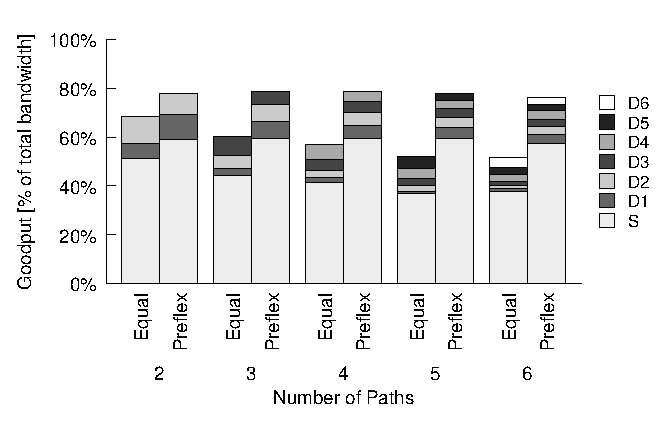
\includegraphics[width=4in]{figures/cate/diffbw}
    \caption{Goodput relative to $B$ achieved by each server for different capacity links.}
    \label{fig:goodputdiff}
\end{figure}

Where bottleneck bandwidth is unequal however equalisation proves inadequate. 
Once again comparing goodput (figure \ref{fig:goodputdiff}) we highlight two significant shortcomings of equalisation which \ac{PREFLEX} overcomes. 
Firstly, goodput for $S$ drops as $N$ increases. 
Unable to realize it is overloading a path, equalisation is reduced to sending traffic over each link at approximately the same rate as the most congested link. 
In contrast, \ac{PREFLEX} detects congestion and adapts accordingly. 
Secondly, the incorrect distribution of traffic due to equalisation in $S$ distorts the goodput of others servers. 
While in \ac{PREFLEX} goodput from $D_{1-N}$ is perfectly balanced, with equalisation traffic crossing the most congested links are directly affected by another domain's inability to distribute its traffic appropriately.
It may seem unfair to judge equalisation for cases where there is a mismatch in link capacity, however this mismatch between link weight and path capacity arises regularly as operators continue to adjust traffic engineering according to local conditions, with little thought spared for the impact this may have further downstream.

\begin{figure}
    \centering
    \includegraphics[width=3.2in]{figures/cate/duration}
    \caption{Mean average flow completion time for equal and differing bottleneck links.}
    \label{fig:duration}
\end{figure}

This impact is in turn perceived by users, who experience longer flow completion times, as shown in figure \ref{fig:duration}. 
In the equal bandwidth case the flow completion time is similar for both balancers.  
Where bandwidth differs however, \ac{PREFLEX} outperforms equalisation and maintains a stable performance when balancing over all six paths.  
This shows that the algorithm scales well as the number of available paths increases. 


\section{Conclusions}
\label{section:malawi:conclusion}

The focus of this work has been on elucidating the main factors that affect flow throughput, but which escape traditional TCP modelling based on end-to-end loss and delay. 
In particular, we explore the changing role of \emph{host limiting}, \emph{application pacing} and \emph{receiver shaping} in defining flow rates across five years of transit traces.
Our results show that for the observed link, over \emph{half} of all inbound TCP traffic can be ascribed to one of the aforementioned constraints.
We show that continuing OS upgrades have progressively lifted the artificial throughput constraints imposed by the host stack. In particular, windowscale negotiation for inbound traffic increased threefold in the observed period, covering over 80\% of all observed bytes by 2012; in addition, we show that buffer sizes have also shown continuing increases over time.

These developments have significantly improved throughput, in particular for smaller flows. However, we also found evidence of throughput limiting effects independent from available end-to-end capacity. This means that no amount of bandwidth will directly improve TCP rates for a considerable amount of traffic.
We show that application-driven techniques for chunked transfer are widely used, accounting for 40\% of all inbound traffic observed in 2011.
%, and that this behaviour is endemic to a wider range of stakeholders than in 2007.
Finally, we uncover evidence of significant receiver traffic shaping prior to 2011 based on the modification of the receiver advertised window in a bid to curtail congestion.
%Uncover evidence of receiver shaping during period of relative contention.



\chapter{A longitudinal analysis of \acs{TCP} traffic}
\label{chapter:malawi}

\renewcommand{\locfolder}{\chapfolder/malawi}
\section{Introduction}

% generic "failures are bad"
Despite being broadly designed for robustness, the current Internet architecture remains remarkably vulnerable to failures.
Managing faults effectively poses a significant operational challenge, in part because faults differ widely in both source and nature, potentially occuring at any layer of the stack and along any element along a path.

% neither is transport
\LOREM
\LOREM

% network methods
Given the commercial nature of the Internet, the onus of providing resilience has instead shifted to network operators.
Traditionally this has been achieved by overloading the routing architecture.
The deployment of real time applications with harder constraints on reliability coupled with better failure detection methods embedded in linecards have provided both the motivation and the means for achieving sub-second recovery within IGP networks \cite{}.
Even with reduced recovery times however, the transient effects of routing changes can still disrupt the forwarding path. 
Under such cases diverse proposals such as Fast Re-Route \cite{}, Loop-Free Alternate next hops \cite{} or Packet Re-cycling \cite{} can provide repair paths for use between the detection of a failure and the convergence of the routing process.

Unfortunately, such methods are rarely sufficient.
Firstly, their application is circumscribed to individual domains, and as such cannot provide end-to-end coverage in a federated, best-effort Internet.
Secondly, there are many faults which do not directly pertain to routing, such as middlebox misconfiguration or hardware malfunctions, and as such go undetected.
Finally, reparation often disregards and potentially disrupts the transport layer by causing out-of-order delivery of packets.

% why now. datacenter, SDN
\LOREM
\LOREM
\LOREM

% layout?
\LOREM
\LOREM


%Outside their networks however, operators are reduced to negotiating service level agreements with their own providers who are invariably unable to cater for such specialized demands \cite{}.
%Even if such terms were met, the Internet architecture provides limited visibility beyond one's own domain.
%This opaqueness, in addition to the fact that failures themselves may be distributed in nature \cite{}, severely limits the ability for a customer network to trace remote problems to a single source \cite{}.
%With no means to hold providers accountable for failures, there is little to enforce the terms of a truly end-to-end SLA.
%
%Unfortunately, such intradomain methods 


%Alongside this increased centralization of resources comes a heightened sense of accountability.
%The commercial nature of the agreements between customers and cloud hosting companies such as AWS \cite{} often involve the establishment of service level agreements.
%Even where such agreements are not explicit, such as the base option of tiered services such as Dropbox or Heroku, there is an inherent need to minimize the impact of outages -- non paying customers may be less demanding, but they are also less sensitive to the switching cost incurred in changing service provider.
%
%Unfortunately, the federated, best-effort nature of the Internet seemingly does not lend itself to such high expectations.



%Under such cases, a network operator is currently expected to detect, repair and recover from such faults.
%Detection often requires scale -- the reliability with which a fault can be identified relies on the proportion of traffic affected. 
%In many cases, faults affecting single flows may go undetected by the network.
%Once detected, reparation varies according to the nature and origin of the fault.
%For some cases, such as intradomain routing, this process is often automated and robust.
%For many others however, such as faulty hardware or misconfigured devices, recovery is difficult and error-prone.
%In either case, the amount of time expended in detection and repair can often preclude recovery, since most flows will terminate after successive timeouts.
%

%Fueled largely by economies of scale in both software management and hardware acquisition and maintenance, the emergence of cloud computing and content distribution networks has lead to a profound shift in Internet traffic.
%
%
%Whereas the advent of broadband connections init
%In contrast to the highly distributed nature of peer-to-peer software which 
%
%
%For one, never has so much been distributed by so few to so many.
%% AS dist graph
%% netflix
%
%\LOREM
%
%% Accountability, resilience

%All intervening equipment is subject to failure along a network path, with recovery time depending not only on \emph{what} happened, but also \emph{where}.
%Within their networks, operators are free to instrument and deploy arbitrarily complex tools to meet requirements. 
%This freedom has lead to a proliferation of proposed improvements in resilience for intradomain settings \cite{}.


%The establishment of SLAs for network availability have traditionally been prefered within the telecom industry in particular, and represent one possible approach to ensuring resilience. An alternative approach is offered by the end-to-end principle. 
%Since end hosts possess both inherent knowledge of application needs and fine-grained measurements on end-to-end path characteristics, the transport layer is often identified as a more natural fit for dealing with fault tolerance at an Internet scale.
%Both SCTP \cite{} and MPTCP \cite{} enable transparent fail-over through multihoming.
%In spite of providing significant features, neither is likely to be widely deployed in the near future: the former lacks critical middlebox support, while the latter is still undergoing standardization.
%Furthermore, the requirement for end-host multihoming has also posed a barrier to deployment.
%Finally, all transport approaches to fail-over confine knowledge of faults within an individual flow: each flow must detect failures independently, even when many flows are affected by the same fault.
%


% Transport is not the answer

% Can we do better with SDN?


%A default forwarding plane, corresponding to the label 0, must be defined and cater for all traffic destinations.
%As with existing routing infrastructure, this single default plane will suffice for most traffic.

%Invariably however, path failures will arise which may affect any number of flows.
%Rather than expecting the network to address end-to-end failures, hosts are allowed to proactively request an overlay plane from the network.





\section{Related work}
\label{section:malawi:related}

Despite their inherent value, longitudinal studies of Internet phenomena are rare. 
Over its short lifespan the Internet has been shaped as much by technological change as by political and commercial realities. 
This dynamic nature does not lend itself to observational studies where data must be collected and curated over long periods of time, and has resulted in a scarcity of relevant datasets. 
What few exceptions exist often stem from collaborative research efforts, such as CAIDA \cite{CAIDA} or Oregon Routeviews \cite{routeviews}. 
The usefulness of these datasets however can be severely affected by the need for data privacy. 
The dissemination of interdomain routing information, where no such requirement exists, has assisted in a wealth of research on wide ranging topics, from quantifying path diversity \cite{Oliveira:2009p203} to locating Internet bottlenecks \cite{Hu:2004p96}. 
In contrast, longitudinal datasets relating to passive measurements have nurtured a much smaller community of researchers often focusing on characterizing traffic \cite{Fontugne:2010p413}. 
Stripped of the locality contained within IP addresses however, researchers are left unable to relate these findings to a wider context.
Instead, cross-sectional studies characterizing traffic aggregated by location are frequently conducted under different contexts \cite{Ager:2011:WCC:2068816.2068870}, but lack the temporal perspective only longitudinal studies can afford. 
Efforts to characterize the spatial properties of traffic over time \cite{Dhamdhere:2011p428,Labovitz:2010:IIT:2043164.1851194,Cho:2008:OSC:1544012.1544024} have defined the changing of Internet topology and traffic alike but fall short of relating such shifts with their impact on relevant metrics such as loss or delay. 

% other work since
This chapter builds on a wealth of prior work on understanding Internet traffic and serves as a reappraisal of significant past contributions.
Flow characteristics and \ac{TCP} behaviour at large are subject to frequent reassessment \cite{Zhang:2002p85}.
Of particular relevance to the current work are passive studies which delve into the inner mechanisms of \ac{TCP}.
In \cite{Jaiswal:2004p242}, Jaiswal et al.\ infer the sender's congestion window by identifying the congestion control variant from the behaviour observed during loss recovery.
The use of separate state machines for each variant however proves unscalable given the many flavours of \ac{TCP} congestion control which have since been deployed.
In \cite{Lan:2006p566}, Lan et al.\ analyse flows according to size, duration, rate and burstiness and characterise the observed correlations for heavy-hitters specifically,
uncovering evidence of increased application influence on flow rates and burstiness and consequently suggest treating flow size and duration as independent dimensions.

One central aspect to the analysis of \ac{TCP} behaviour is the estimation of \ac{RTT} from packet capture data. 
In addition to SYN-based methods, Shakkotai et al.\ \cite{Shakkottai:2004p408} evaluate further techniques to estimate the \ac{RTT} of a unidirectional flow. 
The \textit{rate change} method establishes a relation between the \ac{RTT} and the increase in sending rate, assuming linear window increases during congestion avoidance. 
Unfortunately, this assumption no longer holds, both due to the proliferation of less conservative congestion control algorithms such as CUBIC \cite{Ha:2008p471}, and due to application-driven flow control. 
An alternative is the use of frequency-domain techniques \cite{Veal:2005p412,Lance:2005p565,Qian:2009p429}, which are a natural fit given the self-clocking nature of \ac{TCP}. 
However, a common difficulty with the application of spectral analysis is extracting the fundamental frequency which corresponds to the \ac{RTT} in the presence of noise. 
In applying the Fourier transform to inter-packet arrival times, for example, Qian et al.\ \cite{Qian:2009p429} note that less than half of all flows have distinguishable \textit{flow clocks}; likewise, the \ac{FFT}-based \ac{RTT} recovery was found to be unreliable even after pre-processing available data to enhance inherent periodicities.

% topological influence
Finally, it is important to elucidate what changes in traffic properties are intrinsic to \ac{TCP} and data transfer, and which ones arise from large-scale changes in the \ac{AS}-level topology of the Internet. 
In the decade since publication of \cite{Zhang:2002p85}, the Internet has undergone significant changes, shifting from a broadly hierarchical form to a flatter, more interconnected structure \cite{Labovitz:2010p175,Ager:2012p567}.
Given the longitudinal nature of this chapter and its focus on interdomain traffic in particular, the insights provided by these studies on the macroscopic effects of content consolidation are discernible within the studied dataset, and as such are a source of validation for many of the observations herein.

\section{Dataset}
\label{section:malawi:dataset}

This section provides an overview of the datasets used in this work and some of the data processing required before approaching the longitudinal study of Internet traffic rate limiting. We use the original, unanonymised traffic traces of the MAWI \cite{mawi} dataset, a set of daily traces from the WIDE backbone network which provides connectivity to universities and research institutes in Japan. Traffic is captured daily for 15 minutes starting at 14:00JST. Although this dataset extends back largely uninterrupted from late 2001, we focus on just over five years of data following a network upgrade to the monitored link on October 2006.

The monitored link carries mostly trans-Pacific commodity traffic between WIDE customers and non-Japanese commercial networks. 
We will refer to traffic towards WIDE as \emph{inbound} traffic, whereas traffic originating from within WIDE is referred to as \emph{outbound} traffic.

\begin{table}[!htp]
\scriptsize
\centering
    \begin{tabular}{r|cccccc}
        & & TCP data & \multicolumn{2}{c}{Traffic (TB)} & \multicolumn{2}{c} {Count ($\times10^3$)} \\
        Year & Days & flows (x$10^6$) & In & Out & AS & Prefixes \\
        \hline
        2006 & 91 & 20.52 & 0.43& 0.45 & 10.90 & 56.86\\
        2007 & 350 & 102.56 & 2.11 & 2.49& 17.21 & 113.79\\
        2008 & 358 & 112.26& 2.43 & 2.10& 24.74 & 156.54\\
        2009 & 364 & 113.97& 2.48 & 2.53& 19.71 & 143.87\\
        2010 & 365 & 113.70& 2.58 & 3.43& 20.38 & 148.03\\
        2011 & 358 & 114.74& 3.44 & 5.14& 19.99 & 140.56\\
        \hline
        Total & 1886 & 5777.55 & 13.50 & 16.14 & 34.12 & 341.22\\
    \end{tabular}
    \caption{\label{table:overview}Overview of traced MAWI dataset 
}
  \vspace{-3mm}
\end{table}

A preliminary overview of the dataset used is provided in table \ref{table:overview}. 
In total, 5.7 billion flows containing data are traced over five largely uninterrupted years; this represents approximately 30 terabytes of TCP traffic. For the purposes of this work, we will focus exclusively on inbound traffic, 60\% to 80\% of which originates from port 80, referring only to analysis of outbound traffic when providing a wider context for our findings.
Given the sender side plays a critical role in shaping traffic, analysing traffic for which the source is restricted to a small set of networks within Japan would be of limited use in accurately depicting traffic trends at large.
We instead fix hosts within Japan as sinks, thus sharing a similar perspective on inbound traffic as many other networks. 

\subsection{Tracing TCP Metrics}

All TCP flows are reassembled and analysed for each daily trace.
In addition to the five tuple used to define each connection, we impose two additional restrictions: a contiguous sequence number space and a three minute timeout. These restrictions are helpful to deal with port reuse and unterminated flows respectively.  
Although the total number of TCP flows increased dramatically in 2011, the number of flows \emph{for which data payload was seen} has remained stable, averaging over 100 million data flows traced per year.  

There is much prior work with regards to reconstructing TCP flow from passive measurements and using this information to understand the end-to-end properties of traffic \cite{firstRTT,Jaiswal:2007p233,Rewaskar:2007p195,Shakkottai:2004p408}. However, the MAWI traces impose two constraints which require careful consideration, and ultimately led to the use of a custom TCP tracer. 
The first one is the proportion of bidirectional flows, that is flows, where both forward and reverse path are seen. 
In the dataset used this fluctuates between 40\% and 60\% over five years.
Most available TCP tracers either ignore or are inadequate at processing unidirectional flows. 
The second one is the short duration of each individual trace file. 
At only 15 minutes of line-rate data capture per day, it is wasteful to ignore flows which are not complete. Although the number of flows for which a SYN and FIN in either direction is observed has remained consistently high until late 2011, these flows are normally \emph{mice}, i.e. flows that tend to be brief and which carry little traffic individually. In contrast, most \emph{elephants} (flows that carry significant traffic individually) have durations that exceed that of each trace file. 

%rtts traced
%While many metrics are extracted for each flow, for the purposes of this paper we will focus only on detailing how we collected delay and loss.
%Passive RTT estimates, calculated as the offset between a data packet and its respective acknowledgement, require both directions to be observed at the measurement point. 
%This provides delay estimates between the measurement point and the receiver, as illustrated in figure \ref{fig:synrtts}. 
%For flows where data is transfered in both directions, we will obtain in effect two separate estimates, $RTT_{m2a}$ and $RTT_{m2b}$, illustrated in figure \ref{fig:synrtts}. 
%Together they form the total end-to-end delay experienced by end-hosts. 
%For the remainder of this paper, the term RTT will refer to delay between our measurement and destinations outside WIDE. 
%We discard the delay between measurement point and hosts within WIDE for two reasons. 
%It is both negligible for a large proportion of traffic, which is highly concentrated within the Tokyo metropolitan regions and immediate surroundings, and extremely large for a very small subset of hosts located outside Japan, as WIDE has in the past acted as a provider to academic institutions in Indonesia through a satelite uplink. 
%By decoupling both directions we focus purely on the changes in delay to locations outside Japan. 
%This incurs a reduction in the range of destinations for which we can obtain estimates - only bidirectional traffic can be traced this way. 
%For the set of destinations we will study in this paper, we shall show that this reduction is small. 
%For tracking delay changes for unidirectional traffic for other purposes, MALAWI includes RTT estimates extracted from the SYN exchange.

Loss is inferred by accounting for \emph{retransmissions} in the upstream data and \emph{out-of-order packets} in downstream data; for the remainder of the paper we will refer to the \emph{end-to-end loss} as the sum of out of order and retransmitted data bytes over the total data bytes in a given direction.
% XXX: remove RTT ref?
%Tracking both retransmissions and out-of-order packets accurately requires a reliable RTT estimate, which can only be obtained for bidirectional flows. We forfeit some precision by not taking this into account, as we wish to be consistent in how we estimate both metrics independently of the type of flow and aggregation. 
Pragmatically, we found this to be an adequate indicator of loss --- with the exception of \emph{hanging} TCP connections. 
In these cases where connectivity is lost, a host will proceed to retransmit packets while performing an exponential backoff. 
Although this results in negligible overall traffic, it can significantly skew the inferred loss ratio for uncommon destinations for which little traffic exists. 
To account for these cases, we imposed a 3-second timeout on retransmissions after which we consider the congestion feedback loop to be broken. 

Each daily trace in the dataset is processed from a packet level capture into a collection of flow level statistics. 
This gives us insight into the end-to-end characteristics of traffic. However, since a core objective of this work is to augment this time-based information with data describing the endpoints of each flow, aggregating by location is also required. 

\subsection{Aggregating by Location}

Location information is added by mapping the original source and destination IP addresses to its geographical and topological counterpoints. 
We use the \emph{routeviews} archives to reconstruct the mapping between each IP and both AS and network prefix; bi-hourly dumps of BGP RIBs are available in the WIDE archives since mid 2003. 
We reconstruct a daily RIB based on the views provided by contributing ASes, in particular IIJ and APNIC. 
Since exact routes are not disclosed (there is no record of local policy), we have no knowledge of the route taken by packets; this of course does not hinder our ability to consistently map IPs to ASes. While discrepancies in AS destinations exist between different routeviews contributors, we note that this happens almost exclusively on prefixes for which no actual traffic is seen. 

Mapping IP to country is done through the use of GeoLite \cite{maxmind}, a commercial geolocation database. 
While the accuracy of this solution is often disputed, we are not overly concerned with locating traffic at a fine granularity. 
We will mostly focus on tracking traffic by country and, for larger countries such as the U.S, by region, in order to capture shifts over time.
GeoLite proves adequate on both counts.
The archive for geolocation data only extends to 2009, before which we must rely on the earliest match. 
Additionally, we verify if the destination or source AS have maintained the same administrative mapping up until mid 2009 in the relevant RIR (regional internet registry) archives; otherwise, we do not associate a flow to a geographical location.
% bridging paragraphs to save space.
After associating flows to country, region, AS and network prefix for both source and destination IPs, we aggregate flow statistics over each location identifier. 
This generates a daily collection of location identifiers and associated flow properties, from which we can sketch the geographic and topological properties of the dataset over time.

\section{Methodology}

Providing a macroscopic view on where traffic originates from, and in what quantity, can be achieved by simply binning packets into flows and accumulating byte counts over geographical or topological locations. 
Uncovering application layer characteristics (i.e. \textit{how} traffic is sent) is a more complex problem that requires additional methods to reverse engineer transport behaviour.
The aim of this section is to describe a process which distinguishes those flows which have their throughput limited by mechanisms other than the usual \ac{TCP} response to loss and delay.
Each flow can be characterized as being either application paced, in which the sending application is limiting the data provided, host limited, whereby local constraints at either end host cap throughput, or receiver shaped, in which an artificial constraint is imposed by either a middlebox or receiver.

The classification proceeds in stages. 
Before classification, it is necessary to reconstruct the RTT of the flow if the flow is not bidirectional.  
This is achieved in section \ref{subsection:malawi:PeriodicEnhancement}. 
Because the sender's TCP state machine cannot be directly observed it is necessary then to estimate the size of the congestion window by observing the number of unacknowledged bytes in flight (\textit{flight size}).
This reconstruction is described in section \ref{subsection:malawi:flightAggregation} and provides the basis for flow classification. 
Flows are then checked in turn to see if they are application paced, host limited or receiver shaped and classified as belonging to the first of these classes for which they fulfill the necessary conditions.
Flows in none of these classes are either limited only by the network (delay or loss conditions) or are insufficiently large to trigger any further constraints.

\subsection{RTT Estimation}
\label{subsection:malawi:PeriodicEnhancement}

Building on prior work presented in section \ref{section:malawi:related}, this section proposes an algorithm that scalably recovers the RTT from one-directional traffic traces. 
% XXX: below implies microflights were used, but these aren't described (remove as appropriate)
Although \ac{RTT} estimation is a difficult problem, simplifying assumptions can be made.
For the \ac{MAWI} dataset most \acp{RTT} are relatively large, with the closest neighbouring country, South Korea, roughly 40ms away.
By only processing bidirectional traffic from Japan, the expected \ac{RTT} range can be reduced for all other traffic.
The recovery mechanism then enhances the natural periodicity of traces and scalably constructs flights associated with specific application and protocol behaviour.
In the following the mechanisms required by these two goals are described. 
%
% Why does this work?
%
In normal operation, many \ac{TCP} operations involve request-response cycles between two endpoints in which the \ac{RTT} $T$ provides a natural \emph{clock}.
Hence, the most natural way to estimate \ac{RTT} from \ac{TCP} traces is to correlate requests and responses exchanged in both directions. 
If only one direction of data is observed however, $T$ cannot be directly observed. 
Instead, it must be estimated from the way in which \ac{TCP} packets cluster in time due to the batching of request-response operations.

The \ac{TCP} \ac{cwnd} determines the number of unacknowledged bytes that a \ac{TCP} flow may maintain at any point in time. 
This can be referred to as \emph{bytes in flight} because they are in transit between the sender $S$ and the receiver $R$; an equivalent definition applies for the number of \emph{packets in flight}. 
Once $S$ has transmitted \ac{cwnd} data bytes, it will refrain from transmitting more until either some bytes are acknowledged by $R$ or \ac{cwnd} is increased by the sender. 
In the absence of losses, neither of these events can happen until a \ac{TCP} \ac{ACK} is received; this immediately reduces the number of unacknowledged bytes, but may also lead to a significant \ac{cwnd} increase (during e.g. \emph{slow start}). 
% XXX: number of unacknowledged bytes reduced, or CWND?
In the presence of losses, however, bytes can be re-sent if a packet is timed out and considered lost; in this case, the number of unacknowledged bytes is reduced.

%
% What is our main contribution, algorithmically speaking?
%
The main difficulty associated with one-sided TCP flow reconstruction is as follows.
Let $t_1, t_2, \ldots$ be a set of times at which packets $p_1, p_2, \ldots$ were observed at $S$ en route to $R$.
Suppose that a packet $p_j$ of size $b$ is observed at time $t_j$.
In addition, suppose that approximately one RTT $T$ later, the sender $S$ receives an ACK $a_j$ from $R$ for the $b$ bytes of $p_j$.
At this point, the TCP stack in $S$ will decrease the number of unacknowledged bytes by $b$, thus opening the possibility for sending additional traffic to $R$.
This can lead to another packet $p_k$ to be transmitted; let this packet be observed at time $t_k$ as it is sent towards $R$.
Assuming that processing delay is insignificant, the RTT experienced by $p_j$ can be approximated as $T \approx t_k - t_j$.
Now consider what happens if packets are only observed in the $S \rightarrow R$ direction.
Under such conditions, it is not possible to ascertain whether $p_k$ was sent explicitly as a result of $S$ receiving the unobserved \ac{ACK} $a_j$, or whether it was sent as a result of an \ac{ACK} $a_i$ associated with a previous packet $p_i$ rather than with $p_j$.
If, however, a packet $p_l$ is eventually observed that did result from the reception of $a_j$, the \ac{RTT} can be estimated as $T \approx t_l - t_j$ with $t_l > t_k$.
Following this same reasoning, approximately one \ac{RTT} later a packet $p_m$ will be observed for which $2T \approx t_m - t_j$; this can potentially continue for as long $S$ has data to send and $R$ continues sending \acp{ACK}.
This is the underlying reason that \ac{RTT}-related periodic regularities arise when considering the timestamps of observed packets \cite{Qian:2009p429}.

The reasoning above is at the heart of the proposed algorithm to improve \ac{RTT} recovery by enhancing packet stream periodicity. 
Assume that a packet $p_j$ is observed at time $t_j$. 
Considering the set $\mathcal{T}_j$ of all values of $\Delta t = t_k - t_j$ for every $k > j$, it is apparent that it will include estimates not only for the \ac{RTT} $T$, but also for all its multiples $2T, 3T, \ldots$ 
If $t_l-t_k \approx T$ and $t_k - t_j \approx T$ then it follows that $t_l - t_j = 2T$, and this value will also be included in $\mathcal{T}_j$. 

By maintaining a set $\mathcal{T}_j$ for every packet $p_j$ observed, at least some of its values will correspond to estimations of multiples of the \ac{RTT}. 
It then follows that by creating a set $\mathcal{T}$ that includes values calculated starting from every packet $p_j$ so that $\mathcal{T} = \cup_j \mathcal{T}_j$, numerous estimates for $2T, 3T, \ldots$ will also be included. 
Hence, the probability density function $H(t)$ of the values in $\mathcal{T}$ should show peaks around multiples of the \ac{RTT} (see Figure \ref{fig:histogram}). 

\begin{figure}
  \centering
  \includegraphics[width=0.8\textwidth]{figures/malawi/rttbin.pdf}
  \caption{$H(t)$ for flow displayed in Figure \ref{fig:hostlimited}. The horizontal line delimits $\overline{H}$ while the highlighted bin denotes the bidirectional RTT estimate.\label{fig:histogram}}
\end{figure}

%
% Explain why did we use FFT
%
The algorithmic recovery of $T$ from $H(t)$ presents additional challenges. 
In particular, $H(t)$ may include a large number of \ac{RTT} multiples, and a peak will be found for all of them. 
Crucially, all these peaks may be of comparable magnitude, complicating the task of selecting a single peak.
Moreover, these peaks need not be very pronounced, with histogram bins in close proximity of the peaks have very similar values as the peak itself. 
As such, taking \ac{RTT} candidates directly from $H(t)$ may result in a large set of similarly-valued bins situated around a peaks at multiples of the \ac{RTT}. 

Three recovery algorithms for $T$ are attempted.
First, as a baseline, the highest peak in $H(t)$ is selected as a candidate for $T$. 
In addition, expanding upon the work of Qian et. al. \cite{Qian:2009p429} a frequency-domain representation of $H(t)$ is used to identify $T$. 
This is done by selecting the highest peak of $|\hat{H}(\omega)|^2$, the \emph{energy spectral density} of $H(t)$ (i.e. the norm squared of the Fourier transform of $H(t)$). 
Finally, a custom utility-based technique that operates directly on $H(t)$ is proposed which achieves superior performance to both of the aforementioned methods.

%\subsubsection{FFT-Based RTT Recovery}
%We extract periodicity information from $H(t)$ by looking at $\hat{H}(\omega)$, the \emph{energy spectral density} of $H(t)$. Formally, $\hat{H}(\omega)$ is defined as the norm squared of the Fourier transform of $H(t)$, so that $\hat{H}(\omega) = |\mathcal{F}(H(t))|^2$. Using $\hat{H}(\omega)$ markedly improves the quality of our RTT estimation because the frequency peak corresponding to the RTT usually accounts for a much larger proportion of the total frequency domain energy than other peaks in $\hat{H}(\omega)$, leading to a much simpler discrimination of the true RTT. However, due to RTT changing during the lifetime of a flow, and also due to the expected noise associated with real-life data sources, $\hat{H}(\omega)$ can also occasionally include large peaks at frequencies unrelated to the RTT. In order to filter these out, we take a set of 10 frequency candidates from $\hat{H}(\omega)$, and use their associated periods as RTT candidates in our flow reconstruction algorithm (see Section \ref{
%subsection:malawi:flightAggregation}). We then select that RTT candidate which exhibits the smallest error, that is, that one which yields closest agreement with observed data.

%
% Algorithmic hacks
%
%To streamline our algorithm for streaming use, we use the following heuristics and approximations. Firstly, we define a range $[T_{\min}, T_{\max}]$ representing the range over which we find the RTT values of interest. Then, for each packet $p_j$, we build a subset $\mathcal{T}_j'$ of $\mathcal{T}_j$ by including all values of $t_j - t_k < T_{\max}$. We then generate $\mathcal{T}' = \cup_j \mathcal{T}_j'$ and approximate $H(t)$ by considering a histogram of the values in $\mathcal{T}'$. As usual, we do this by counting the frequency with which its values are observed in the ranges $[0,\tau)$, $[\tau, 2\tau)$, $[2\tau, 3\tau), \ldots$ where $\tau$ is the time resolution required. 


\subsubsection{Utility-Based RTT Recovery}
\label{sect:utilityBasedRecovery}

This method relies not on the identification of periodicities, but on explicitly matching experimentally found signatures. 
To this end, we consider the peaks of $H(t)$, which are then considered RTT candidates.  
However, trivial discriminators (such as simply selecting the highest peak) are not reliable. 
In this case, it was found experimentally that repeatable peaks and troughs also occur at multiples and sub-multiples of $T$, with the most important ones being $\frac{T}{3}$, $\frac{T}{2}$, $T$ and $2T$. 
We design this detection algorithm around the idea that a given pattern of peaks and troughs can identify $T$.

If we define $\overline{H}$ as the mean height of $H(t)$, we can define a per-peak utility function $p(t)$ so that 
\begin{equation*}
p(t) = 1.0 - \exp\left(-2.0 \left(\frac{H(t)}{\overline{H}}\right)\right) \mbox{.}
\end{equation*}
This function has several advantageous properties: it is 0 if $H(t)$ is zero, 1
if $H(t)$ is infinite, and $0.5$ if $H(t) = \overline{H}$.  In other
words it is a measure of the \emph{peakiness} of the data, with $p=1$ identifying
an infinitely high peak, $p=0$ identifying an empty histogram bin (trough), and $p=\frac{1}{2}$ 
implying that $H(t)$ is of exactly average height at that point. We can then score each candidate using the following utility function:
$$
P(t) = 1.5 p(t) + p(2t) - p\left(\frac{t}{2}\right) - p\left(\frac{t}{3}\right).
$$
That is, the candidate RTT $t$ scores highly if it is itself a peak, if it has a peak
at a multiple $2t$, and if it also manifests troughs at submultiples $\frac{T}{2}$ and $\frac{T}{3}$.
The factor of 1.5 was added after observations
showed that the peak at $T$ was the most important factor in determining
whether a candidate was the true RTT. Similarly, additional multiples and submultiples 
were excluded as they showed very limited discriminating power experimentally.

\begin{figure}
  \centering
  \includegraphics[width=0.8\textwidth]{figures/malawi/rttcomp.pdf}
  \caption{Accuracy of RTT estimator when compared to the median value of bidirectional estimate.}
\end{figure}

\subsubsection{Comparing RTT Recovery Algorithms}
\label{sect:comparingRecoveryAlgos}
As described in Section \ref{subsection:malawi:PeriodicEnhancement}, $H(t)$ is calculated in such a way that RTT periodicity is amplified. 
This means that FFT-based techniques could potentially perform better on $H(t)$ than on the packet stream with no pre-processing. 
However, this is complicated not only because $H(t)$ contains periodicities at multiples of $T$, but also discontinuities that generate harmonics at frequency multiples of the RTT fundamental. 
Hence, although the FFT $|\hat{H}(\omega)|$ of $H(t)$ is much cleaner than that of the packet interarrival time series on its own, its maximum peak rarely coincides exactly with the RTT clock (this corroborates reports by Qian et al \cite{Qian:2009p429}). 
Thus, applying the FFT leads to another \emph{peak detection problem} in which the RTT fundamental needs to be extricated from its harmonics and sub-harmonics. 
The trivial solution to this problem, the application of a bandpass filter around the RTT frequency, is of course unfeasible because the bandwidth and 
centring of such a filter depend on the RTT which is itself unknown.
The utility-based algorithm described in Section \ref{sect:utilityBasedRecovery} can hence be applied in either the time domain or the frequency domain; we chose to do it on the former on the interest of expediency and lower computational cost.

\newcommand{\RTTHeader}{Below & Above}
\newcommand{\SmallFlowName}{\textless 10MB}
\newcommand{\LargeFlowName}{\textgreater 10MB} 
\begin{table}
\footnotesize
\centering
\begin{tabular}{ p{1.5cm} p{1.2cm} p{0cm} p{.6cm}p{.6cm} p{0cm} p{.6cm}p{.6cm}}
& & & \multicolumn{2}{c}{Peak} & & \multicolumn{2}{c}{Utility-based} \\
\cline{4-5} \cline{7-8}
& Flow size & & \RTTHeader & & \RTTHeader \\
\cline{4-5} \cline{7-8} 
\multirow{2}{*}{Receiver side}  & \SmallFlowName && 4.31 & 9.13 && 4.58 & 6.35
\\ 
                                & \LargeFlowName && 6.72 & 6.43 & 4.97 & 5.33
\\
\multirow{2}{*}{Sender side}    & \SmallFlowName && 2.94 & 8.37 && 3.29 & 4.80
\\
                                & \LargeFlowName && 6.41 & 9.06 && 5.40 & 11.06
\\
\end{tabular}
\caption{\label{table:rttRecovery}Performance of RTT recovery algorithms}
\vspace{-3mm}
\end{table}

The performance of the analysed RTT recovery mechanisms is presented in Table \ref{table:rttRecovery}, that shows the percentage of total flows below and above the RTT range given by the bidirectional estimates.
We separate things for \emph{inbound} traffic (where we are positioned at the receiver side) and \emph{outbound} traffic (where we are positioned at the sender side). The utility-based algorithm is particularly useful to address RTT underestimation for flows over 10MB in size, which is our main objective since precisely that kind of estimation error would interfere with our ability to correctly decouple application behaviour from RTT-scale dynamics.


%For the most part, the utility based method improves on underestimation, which is our main objective since that would interfere with our flight reconstruction (i.e. generate lots of gaps).
%The exception (kind of) is traffic from the sender side, which in our training set (one week per year), had quite a lot of host limited traffic (paced out, no signal to recover).
%In this case, not a problem, since if the flow is long enough multiples of the RTT will still reveal host limitation, but will give us a smaller window..


\subsection{Flow Classification}
\label{subsection:malawi:flightAggregation}

One fundamental precondition to decouple the influence that network loss, host configuration and TCP behaviour has on the throughput experienced by a flow is the reconstruction of the congestion window behaviour of TCP flows on the basis of observed data. 
Unfortunately, the congestion window value is internal to the sender's TCP state machine and may not manifest itself in the absence of sufficient data from the application layer. 
A more easily observed quantity which serves as a reasonable proxy for the congestion window is the number of unacknowledged bytes in flight, henceforth referred to as the \textit{flight size}, which can be derived given an accurate estimate of the end-to-end delay.
The evolution of both flight size and RTT can in turn be used to ascertain to what extent throughput is regulated by limitations imposed at different layers of the networking stack.

% definitions
Given a candidate RTT, we can aggregate a stream of packets with arrival times $t_1, t_2, \ldots$ into a stream of \emph{flights}. 
Intuitively, a flight is a clustered subset of a TCP flow which exhibits its own temporal coherence; alternatively, it can be though of as a series of consecutive packets that were (roughly) generated by the sender as a response to the same protocol operation. 
A flight $f_i$ that begins
with the $j$th packet and ends with the $k$th is defined to have a \emph{total flight time} $\tau_i = t_{k+1} - t_j$. 
The algorithmic selection of initial and final packets in such a way that the resulting flights are indicative of TCP behaviour remains an open problem. 
Since we assume that the RTT provides a natural time frame for the operations of TCP, in the algorithm presented in this work, given an initial packet $\pi_j$ and an RTT estimate $T$, the $k$th (and final) packet is selected to minimise \emph{the flight time error} $e_i = |T - \tau_i|$. 
This mechanism follows closely the methodology described in \cite{Zhang:2002p85}, with the exception that we do not attempt to define flights as being both adjacent and disjoint; rather, we decompose flows into a stream of potentially overlapping flights. 
This helps the algorithm mitigate the deleterious effects of small deviations in the estimated RTT, which alters the properties of each flight. 
Furthermore, since the flight size is continuous in time, it makes little sense to restrict ourselves to a single sample per round trip time.

Having obtained flight information from each flow, we next consider what is the predominant factor that affects its throughput. 
Within the context of TCP, we classify flows as being artificially constrained by three distinct processes: \emph{application pacing}, \emph{host limited} and \emph{receiver shaping}.

\begin{figure}
\centering
  \centering
  \begin{subfigure}{1.0\linewidth}
    \includegraphics[width=1.0\textwidth]{figures/malawi/youtube.pdf}
    \caption{Application paced. \label{fig:youtube}}
  \end{subfigure}\\
  \begin{subfigure}{1.0\linewidth}
    \includegraphics[width=1.0\textwidth]{figures/malawi/hostflow.pdf}
    \caption{Partially host limited. \label{fig:hostlimited}}
  \end{subfigure}\\
  \begin{subfigure}{1.0\linewidth}
    \includegraphics[width=1.0\textwidth]{figures/malawi/awnd.pdf}
    \caption{Receiver shaped. \label{fig:awnd}}
  \end{subfigure}
  \caption{Flight size over time for flows affected by different artificial constraints. \label{fig:kindsOfFlowEffect}}
\end{figure}


\subsubsection{Application Paced Flows}
\label{sssec:app}

A flow whose throughput decreases because it has no outstanding data to send is temporarily limited by the application. 
Flights can be identified as being \emph{application limited} if terminated with a packet smaller than the maximum segment size (MSS) and followed by an inter-arrival time greater than the RTT, as consistent with \cite{Zhang:2002p85}. 
The underlying reason for this defintion is that most TCP implementations will wait some time for subsequent bytes to be written to the socket if the next packet to be sent is smaller than the MSS, unless the TCP\_NODELAY option is set \cite{nagle1984rfc}.

A flow with \emph{application limited} flights however is not necessarily \emph{application paced}. In practice, all flows for which the final packet is observed contain at least one such flight.
For the purposes of our work, we are focused on identifying cases in which throughput is predominantly determined by application behaviour.
One such example is illustrated in figure \ref{fig:youtube}, in which a stream is delivered by periodically writing blocks to the sending socket.
The resulting network-level behaviour is distinct from traditional congestion control: short bursts are interspersed with protracted silence.
Application limited flights, which terminate on non-MSS packets, are highlighted at the end of each burst.

This behaviour is in stark contrast to that exhibited in figure \ref{fig:hostlimited}, where distinct transfers are multiplexed on top of a single transport association over time.
From the perspective of the network, there is little to distinguish the behaviour of such traffic from independent TCP flows.
Application paced connections such as Youtube traffic however exhibit a degree of regularity which can potentially be exploited by the network in predicting demand or smoothing bursts.

In order to identify such recurring behaviour, we identify flows as being \emph{application paced} if the period between bursts terminated by \emph{application limited flights} is consistently under 10 seconds and the standard deviation of the intermediate pauses is under one second.
This definition in particular purposely ignores flows which exhibit long silence periods due to user interaction, and follows closely the behaviour historically associated to Youtube streaming in particular.

\subsubsection{Host Limited Flows}
\label{sssec:host}

Given sufficient bandwidth and traffic to send, a flow may encounter local constraints at either end-host which cap its throughput. 
For instance, the buffer space allocated on both the sender and receiver side is often pre-configured, and it is common practice to tune these values down on popular servers and managed infrastructure in a bid to conserve memory or bandwidth.
A receiver is also limited in the window size it can announce to the remote sender; if the windowscale option \cite{jacobson1992tcp} is not negotiated during the TCP handshake, the advertised window cannot exceed 64KB.

In both cases, a local decision by either host can determine the upper bound of the flow rate.
These \emph{host limited} cases are characterised by a constant window size over time.
The methodology described for flight aggregation at the beginning of this section typically generates a large number of flights, representing many likely combinations given a base RTT estimate.
In order to identify the flat-lined behaviour of a host limited flow, we first filter the flight stream to remove some of the uncertainty derived from small fluctuations in the RTT.
We then select the maximum flight size observed for each RTT interval, and declare a sequence of flights to be host limited if the same maximum was observed over six consecutive RTTs (this is twice the period suggested in \cite{Zhang:2002p85}).
In practice, increasing the period over which the maximum window size is tracked allows us to more accurately discern between host limited behaviour and more conservative bandwidth probing, such as that performed during the convex phase of TCP CUBIC \cite{Ha:2008p471}.

A flow may be host limited for only brief periods of its lifetime, as illustrated in figure \ref{fig:hostlimited}.
To filter out such cases where host limitations are not the predominant factor in defining flow throughput, we further enforce that in addition to host-limited flights, the average window size must over a flow lifetime should be within 10\% of the inferred host limit, which is not the case in figure \ref{fig:hostlimited}.

In practice, flows can exhibit both application pacing and host limitations, with bursts being sent at a capped window size followed by application pauses.
In such cases, a flow will still be classified as being \emph{application paced} if it meets the requirements set out in the previous section, as doing so provides evidence that it controls throughput in spite of the degraded performance provided further down the stack. 
This line of reasoning applies equally to the occurrence of sporadic loss; so long as block delivery is ensured within the timeframe dictated by the application, it remains in control.

\subsubsection{Receiver Shaped Flows}
\label{sssec:rec}

A flow which is neither \emph{application paced} or \emph{host limited} can still be artificially constrained by flow control (rather than by congestion control).
Traditionally, in TCP the sender is responsible for regulating throughput. 
However, the receiver can also shape throughput by manipulating the \emph{advertised window} announced on every acknowledgement.
Such receiver-window auto-tuning has been available on Windows operating systems since Vista \cite{vistaReceiveWindow}, and can also be leveraged by middleboxes in order to throttle inbound traffic \cite{appEx}.

In order to evaluate the potential impact of such behaviour, we further propose a heuristic to identify receiver-shaped traffic.
For flows in which both directions of traffic are observed it is possible to correlate the evolution of the advertised window with the size of reconstructed flights.
Figure \ref{fig:awnd} displays an example of a receiver-shaped connection, in this case throttled by an intermediate middlebox.
Since the advertised window may be fluctuating, it is not always obvious which of the many updates were effectively applied by the sender as successive values supersede each other.
An example of a reconstructed flow which is subjected to receiver shaping is displayed in Figure \ref{fig:awnd}.

For flows in which both directions are observed, it is possible to classify flights as being receiver-shaped if there is a statistically significant correlation between the advertised window size and the maximum flight size observed.
Harnessing the stream filtering used in detecting host limited behaviour, we perform such analysis over a sliding window of 10 RTT intervals.
A flight is flagged as being receiver shaped if the correlation between receiver window and flight size is statistically significant; a flow is considered to be predominantly receiver shaped if over half of its flights are flagged as such.
We do not perform this covariance analysis on flights which contain out-of-order or retransmitted packets. 
In these cases, both the receiver and sender window sizes are correlated \emph{by definition}. 
In the former case, the receiver buffer will temporarily fill expecting the next packet in sequence, in the latter case, TCP will reduce its window.

Given that receiver shaping classification requires correlating information in both directions of a TCP connection, it will come as no surprise that the absence of the reverse path can introduce false positives into our measurements. 
This happens because any given flow might be receiver shaped in such a manner that the heuristic erroneously attributes its behaviour to host limitations. 
In the absence of additional evidence, this misclassification is difficult to detect explicitly. 
Instead, we calculate the ratio of receiver shaped flows which would have been incorrectly identified if the reverse path were not observed. 
This error rate can then be used to evaluate the accuracy of classifier results.

\section{Performance Analysis}
%4.1) Balancing between two paths with high loss using fixed time unit
% using only loss-based balance in a simple regime where that works.
% Show how this converges quickly when one path suddenly gains
% background traffic (and hence loss).
%4.2) Balance between several paths with high loss and fixed time unit
% in simple regime where that works.
%4.3) Introduce experiment where equi-path is needed for probing and
% conservative is needed for low loss regime.
%4.4) Introduce experiment where time-scale tuning is needed to get
% good assessment of loss in low traffic regime.

We evaluate \ac{PREFLEX} through simulation in ns-3 \cite{ns3}. 
Since \ac{PREFLEX} balances traffic using loss rather than load, there is a need to emulate the end-to-end behaviour of traffic. 
This proves more challenging than analysis of existing traffic engineering proposals which typically only focus on adjusting load, since we wish to verify the impact of \ac{PREFLEX} on end-user metrics. 

\subsection{Methodology}
\label{section:methodology}

For all simulations we will use the topology displayed in figure \ref{fig:topo}. 
The topology links a client domain $C$ to a server domain $S$ through $N$ paths with equal bottlenecks $L_i$, and total bandwidth $B=\sum{L_i}$. 
While a domain is represented as a single entity in figure \ref{fig:topo}, each domain is composed by a traffic generator connected to a router. 
Client $C$ generates $G$ simultaneous \ac{HTTP}-like requests (or ``gets") from $S$ according to a specified distribution, described at the end of this section. 
As traffic flows from $S$ to $C$, the router within $S$ is responsible for balancing traffic over all available paths.

\begin{figure}
    \centering
    \includegraphics[width=2.5in]{figures/cate/topo}
    \caption{Simulation topology}
    \label{fig:topo}
\end{figure}

Across simulations, as the number of paths increases, total bandwidth $B$ and the number of simultaneous requests $G$ is fixed. 
In this manner we wish to analyze how \ac{PREFLEX} balances traffic as the granularity with which it can split traffic becomes coarser.

Since we are interested in evaluating how \ac{PREFLEX} shifts traffic in response to loss, we introduce additional ``dummy" servers $D_i$ which are connected to $C$ through a single path. 
We partition the total simulation time $T$ into $N+2$ intervals starting on $s_i$, in which $s_0$ and $s_{N+1}$ have no traffic to $D_i$. 
Starting at time $s_i$, client $C$ generates $g_i$ requests to $D_i$ according to the same distribution as used to server $S$. 
All requests to $D_i$ end at time $s_{N+1}$. 
Equation \eqref{eq:si} sets the start time $s_i$ for requests to $D_i$ as a function of total simulation time $T$ and number of paths $N$. 
Likewise, equation \eqref{eq:gi} sets the number of simultaneous requests $g_i$ to $D_i$ as a function of $G$, the total number of requests to $S$, and $N$.
\begin{equation}
s_i = T\frac{i}{N+2}
\label{eq:si}
\end{equation}
\begin{equation}
\theta_i = \frac{\frac{1}{N+1-i}}{\sum{\frac{1}{N+1-i}}},  g_i = G\theta_i.
\label{eq:gi}
\end{equation}

Figure \ref{fig:demand} illustrates the number of simultaneous gets from $C$ to $D_i$ for $N=2$ (used in the example shown in figure \ref{fig:two}) and $N=4$. 
Generating cross-traffic in this manner serves two purposes. 
Firstly, $\sum{g_i}=G$, so independently of the number of concurrent paths, the maximum load in the system is $2G$. 
However, as the number of paths increases, the fluctuation in load for each path becomes smaller, and so we will stress the sensitivity with which \ac{PREFLEX} balances traffic. 
Secondly, the number of requests for each $D_i$ over time is the same. 
Over timescale $T$, equalisation appears to be an acceptable strategy, however within each interval we will show it performs poorly achieve consistent behaviour. 
This is a fundamental limitation of offline traffic engineering, which is calculated over very long timescales and is unable to adapt as traffic routinely shifts.


\begin{figure}
    \begin{subfigure}[b]{.5\linewidth}
        \centering
        \includegraphics[width=2.25in]{figures/cate/dummy2-crop.pdf}
        \caption{$N=2$}\label{fig:1a}
    \end{subfigure}%
    \begin{subfigure}[b]{.5\linewidth}
        \centering
        \includegraphics[width=2.25in]{figures/cate/dummy4-crop.pdf}
        \caption{$N=4$}\label{fig:1b}
    \end{subfigure}
    \caption{Number of requests from $C$ to cross traffic servers $D_i$ for different values of $N$}
    \label{fig:demand}
\end{figure}

We now specify the settings common to all simulations, including those previously shown in figure \ref{fig:two}. 
Total simulation time $T$ is set to $1200$ seconds, while total bandwidth $B$ is fixed at $240$Mbps. 
The number of requests $G$ sent from $C$ to $S$ is set to 240. 
Upon completing, a request is respawned after an idle period following an exponential distribution with a $15$s mean. 
Transfer size follows a Weibull distribution with an average value of $2$MB. 
These values attempt to reflect traffic to a single prefix with a file size that mimics the small but bursty nature of web traffic, which does not lend itself to being balanced by the end-host. 
\ac{PREFLEX} is configured with $\beta_E = 0.05$, $\mu_{min}=0.01/N$ and $\delta=0.005$.

\subsection{Varying bottleneck distribution}

We start by examining the case where all bottlenecks share the same bandwidth, $L_i=B/N$, and compare \ac{PREFLEX} to equalisation, which mimics traffic engineering techniques based on hashing flow tuples and assigning them to a path. 
The goodput, calculated as the total data transfered to client $C$ by flows completed within $T$, is shown for both equalisation and \ac{PREFLEX} methods in figure \ref{fig:goodputeq}. 
While both saturate most available bandwidth, equalisation leads to disproportionate distribution of goodput amongst competing traffic. 
As loss is not equalised over all paths, the amount of goodput achieved by servers $D_i$ differs despite demand being similar.

Equalisation, even when weighted according to local link capacity, is often prone to remote bottlenecks. 
We investigate the effect of differing bottlenecks by repeating previous simulations with the same total bandwidth $B$, but with $L_i$ set proportionally to $B$ in a similar manner to \eqref{eq:gi}, that is $L_i = \theta_i B$.


\begin{figure}
    \centering
    \includegraphics[width=4in]{figures/cate/eqbw}
    \caption{Goodput relative to $B$ achieved by each server for equal capacity links.}
    \label{fig:goodputeq}
\end{figure}

Figure \ref{fig:goodputeq} shows the goodput as a proportion of total link bandwidth for the case where all links have equal bandwidth. 
We vary the number of links $N$, and for each case compare equalisation (as illustrated in \ref{fig:twoequal}) and \ac{PREFLEX} as the balancing methods used. 
The bulk of goodput originates from server $S$, which is the only domain to be connected to all links.  
If traffic is correctly balanced, we expect to see servers $D_{1-N}$ generate the same amount of goodput.

In this scenario, equalisation can be seen as the optimal static TE solution, yet both approaches bear similar performance. 
With no knowledge of topology, link bandwidth or expected traffic matrices, \ac{PREFLEX} is able to adequately mimic the performance of the static TE solution for the case where such an approach is best suited.


\begin{figure}
    \centering
    \includegraphics[width=4in]{figures/cate/diffbw}
    \caption{Goodput relative to $B$ achieved by each server for different capacity links.}
    \label{fig:goodputdiff}
\end{figure}

Where bottleneck bandwidth is unequal however equalisation proves inadequate. 
Once again comparing goodput (figure \ref{fig:goodputdiff}) we highlight two significant shortcomings of equalisation which \ac{PREFLEX} overcomes. 
Firstly, goodput for $S$ drops as $N$ increases. 
Unable to realize it is overloading a path, equalisation is reduced to sending traffic over each link at approximately the same rate as the most congested link. 
In contrast, \ac{PREFLEX} detects congestion and adapts accordingly. 
Secondly, the incorrect distribution of traffic due to equalisation in $S$ distorts the goodput of others servers. 
While in \ac{PREFLEX} goodput from $D_{1-N}$ is perfectly balanced, with equalisation traffic crossing the most congested links are directly affected by another domain's inability to distribute its traffic appropriately.
It may seem unfair to judge equalisation for cases where there is a mismatch in link capacity, however this mismatch between link weight and path capacity arises regularly as operators continue to adjust traffic engineering according to local conditions, with little thought spared for the impact this may have further downstream.

\begin{figure}
    \centering
    \includegraphics[width=3.2in]{figures/cate/duration}
    \caption{Mean average flow completion time for equal and differing bottleneck links.}
    \label{fig:duration}
\end{figure}

This impact is in turn perceived by users, who experience longer flow completion times, as shown in figure \ref{fig:duration}. 
In the equal bandwidth case the flow completion time is similar for both balancers.  
Where bandwidth differs however, \ac{PREFLEX} outperforms equalisation and maintains a stable performance when balancing over all six paths.  
This shows that the algorithm scales well as the number of available paths increases. 


\section{Conclusions}
\label{section:malawi:conclusion}

The focus of this work has been on elucidating the main factors that affect flow throughput, but which escape traditional TCP modelling based on end-to-end loss and delay. 
In particular, we explore the changing role of \emph{host limiting}, \emph{application pacing} and \emph{receiver shaping} in defining flow rates across five years of transit traces.
Our results show that for the observed link, over \emph{half} of all inbound TCP traffic can be ascribed to one of the aforementioned constraints.
We show that continuing OS upgrades have progressively lifted the artificial throughput constraints imposed by the host stack. In particular, windowscale negotiation for inbound traffic increased threefold in the observed period, covering over 80\% of all observed bytes by 2012; in addition, we show that buffer sizes have also shown continuing increases over time.

These developments have significantly improved throughput, in particular for smaller flows. However, we also found evidence of throughput limiting effects independent from available end-to-end capacity. This means that no amount of bandwidth will directly improve TCP rates for a considerable amount of traffic.
We show that application-driven techniques for chunked transfer are widely used, accounting for 40\% of all inbound traffic observed in 2011.
%, and that this behaviour is endemic to a wider range of stakeholders than in 2007.
Finally, we uncover evidence of significant receiver traffic shaping prior to 2011 based on the modification of the receiver advertised window in a bid to curtail congestion.
%Uncover evidence of receiver shaping during period of relative contention.



\chapter{Conclusions}
\label{chapter:conclusions}

The presented body of work identifies opportunities and explores strategies for resource pooling through the application of \emph{re-feedback}.
This chapter summarises these findings in light of the original problem statement:

\begin{quote}
\textit{
Given the nature of Internet traffic, how can the current architecture be realigned to facilitate resource pooling at both network and transport layers?
}
\end{quote}

\renewcommand{\descriptionlabel}[1]{\hspace{\labelsep}\textbf{#1}}
\begin{description}
\item[Efficient]
%cate
\LOREM
\item[Flexible]
%TE, opt-out
\LOREM
\item[Robust]
%inflex
\LOREM
\end{description}

%tip
Resource pooling has evolved to being performed by different stakeholders unilaterally.
End-hosts, network operators and content providers all attempt to pool traffic by differing means, and in a potentially conflicting manner.
While recent work has lent credence to pushing resource pooling towards the edge, this ignores the tussle over how traffic is managed between these stakeholders.
Path diversity is in the network, and operators attempt to exploit it through a combination of route optimization and traffic balancing.
Collectively, these traffic engineering methods assist networks in minimizing the costs incurred by shifting traffic.
Conversely, hosts are increasingly capable of pooling traffic across paths either through the use of overlay networks or multipath congestion control, neither of which necessarily share the objectives of the underlying network.
The problem statement arises from the confluence of these two trends: given the nature of Internet traffic, how can the current architecture be realigned to facilitate resource pooling at both network and transport layers?

\section{Summary of contributions}

The core of the proposed thesis revolves around Internet architecture and as such is of most immediate interest to protocol designers.
The many contributions presented however carry much wider appeal, and can be classified under 

%Network operators, application developers and ?

\subsection{Internet traffic characterisation}

% lit review
This thesis began by providing a broader context within which to frame the evolution of resource pooling.
Chapter \ref{chapter:resourcepooling} traces how successive waves of new stakeholders and novel applications have influenced and shaped the protocols and tools which form the Internet.
Importantly, this chapter highlights traffic management as an architectural afterthought and identifies a pertinent problem:
, with end-hosts, network operators and content providers alike pooling traffic unilaterally through differing means.


% malawi intro
As with any distributed system however, the Internet remains in a constant state of flux.
\LOREM
Chapter \ref{chapter:malawi} provides a significant reappraisal of past work in characterizing Internet traffic
% the flattening, delay 

% rate limitations
The main contribution in this study however was a re-evaluation of commonly held assumptions regarding Internet flow rates by systematically identifying artificial constraints to \ac{TCP} traffic throughput across three categories: \emph{application pacing}, \emph{host limiting} and \emph{receiver shaping}. 
The resulting analysis shows that flow rates are not typically dictated by \ac{TCP} congestion control alone, and has significant implications on how to reason about resource sharing in particular.
The findings equally confirm that \ac{TCP} throughput is mostly determined by the actions of the sender and that continuing \acf{OS} updates have progressively lifted many of the limitations inherent to socket buffer sizes. 
These changes have allowed smaller flows to increase throughput at a far higher rate than larger flows, which are more often than not affected by other mechanisms of traffic shaping.
This means that, although there is a correlation between flow volume in bytes and throughput, the relationship between the two is non-linear and has changed with time.

% implications for resource pooling
These changes were perhaps foreseeable given the all-encompassing nature of the \ac{IP}: the Internet will continue to assimilate the characteristics of the networks it progressively replaces.


% the evolution of existing Internet architecture is less clear.


% tip
%The Internet is in a constant state of flux, as remarkable in its ability to seamlessly accomodate new stakeholders as it is in reinventing itself to meet new requirements. 
%This disruptive nature often hinders our ability to discern between the evolution of the Internet and the ebb and flow of otherwise highly localized events. Under these circumstances, 
%the usefulness of longitudinal studies is twofold: they both offer a perspective on the underlying long term behaviour of a system as a whole, and provide a context under which transient events can be better understood.



Having reconstructed individual flows, the results are aggregated using an external routing information dataset and relate how each aritificial constraint arises in different contexts and affects different stakeholders over time. 
In particular, we show that host limitations have largely been lifted for small flows, with the windowscale option increasing threefold to cover over 80\% of all inbound traffic by the end of 2011. 
Understanding the characteristics of Internet traffic is intrinsic to designing any form of resource pooling.
For long-lived flows, the transport layer has sufficient time to collect information on network state to efficiently pool traffic across multiple paths.
If traffic is dispersed across many prefixes, scaling dynamic traffic engineering may be problematic.
By relating five years of packet traces from an interdomain transit link with topological and geographic information, preliminary results suggest neither is strictly true.
The continuing consolidation of traffic for both inbound and outbound directions allows most traffic to be balanced by manipulating a small number of traffic prefixes.
This work has corroborated previous findings \cite{Labovitz:2010p175} showing a shift in content distribution, with \acf{P2P} applications being slowly replaced by \acfp{CDN} and \acf{OCH} infrastructure.
The novelty has come from being able to relate traffic trends at a finer granularity, both by reconstructing \ac{TCP} behaviour and relating these changes to network prefixes, which can in turn be used to assess the practicality of dynamic traffic engineering methods.


\subsection{Architectural realignment}

% relation to state of art
This thesis set off by exploring the use of re-feedback, originally proposed by Briscoe et al. \cite{}, for purposes other than accountability.
%While the expectation that networks could be held accountable for congestion conferred interesting properties
Removing the expectation that networks would be held accountable for congestion lead to a fundamentally poorer architecture, but one in which enforcement

%is purpose resulted in a significantly

To this end, \ac{LEX} was proposed in \ref{chapter:preflex} as a simplified mechanism for echoing loss back into the network.

The point of departure of this thesis was provided by 
starting point of this 
Loss exposure was since pursued independently by the \ac{CONEX} working group.

% pref
Arguably the single most valuable legacy of this work was in proposing \acf{PREF} as a cross-layer signalling mechanism between the transport and network layer, first presented in chapter \ref{chapter:preflex}.
Within the self-imposed constraints of \ac{IPv4} deployability, the resulting mechanism is necessarily simple, but also shown to be surprisingly versatile, enabling novel end-to-end traffic management techniques such as congestion balancing, presented in chapter \ref{chapter:cate}, and resilient path fail-over, presented in chapter \ref{chapter:inflex}.
Historically, the \ac{PREF} field can be interpreted as a synthesis of the previously sanctioned uses for the same header space: neither strictly abiding by the thesis that end-hosts should independently determine their own \acf{ToS}, nor aligning itself with the antithetical view that the network alone should establish \acf{DS}.
In many respects, it is a stronger ideological heir to the original design philosophy of the \ac{DARPA} internet protocols. 
In deliberating on the success of the latter in \cite{Clark:1988p478}, Clark concludes by identifying shortcomings of the datagram model given requirements which had not originally been contemplated:

While

% lex

% inflex





% tip
Given the Internet architecture should not dictate the outcome of the tussle between end-host and network solutions for resource pooling, the \ac{PREFLEX} architecture attempts to make both aware of each other.
\acf{LEX} transmits information on loss as viewed by the transport layer to network resources, allowing traffic engineering to be performed taking into account end-to-end path quality.
\acf{PREF} offers the ability for the network to select and offer paths to hosts, thereby unlocking the path diversity which already exists at stub domains such as \acp{ISP}, \acp{CDN} and enterprise networks.

\ac{PREFLEX} permits more efficient, reliable and flexible traffic balancing whilst allowing for a range of outcomes in how burden of resource pooling is shared between host and network.
One extreme outcome, in which the network is responsible for all resource pooling, is explored in depth in chapter \ref{chapter:cate}.
A congestion balancer is derived in which \ac{PREFLEX} can reap much of the benefit of \ac{MPTCP} by balancing flowlets according to loss.
Unlike most existing \ac{TE} methods, \ac{PREFLEX} is designed to minimize the impact of route changes on the transport layer and as such is assessed by its impact on transport metrics rather than traffic aggregates.
The use of congestion balancing in the network not only leads to a more efficient use of network capacity, but also a reduction of flow completion times for flows.

    \textbf{Evolution of flowlets}. Recent work on video streaming \cite{Rao:2011p547} , which represents a significant portion of Internet traffic, 
    has shown different sending strategies are adopted depending on the application type (web browser or native) and container (HTML5 or Flash).
    The most popular strategies rely on on/off sending patterns of varying chunk sizes, a form of rate-limiting may affect how efficiently \ac{TCP} can probe for bandwidth.
    A methodology for processing flowlets within the \ac{MAWI} packet traces is being developed to understand the evolution of flowlet sizes within Internet traffic and quantify the potential benefits of balancing at a flowlet granularity as proposed in \ac{PREFLEX}.

{\COMMENT
    %copy pasted from INFOCOM intro
% INFLEX
This paper presents INFLEX, an \ac{SDN}-based architecture for cross-layer network resilience which provides on-demand path fail-over for \ac{IP} traffic. 
The architecture is both unilaterally deployable, providing benefits even when adopted by individual domains, and inherently end-to-end, potentially covering third party failures.
INFLEX operates by allowing an \ac{SDN}-enabled routing layer to expose multiple \emph{routing planes} to the transport layer. 
Hence, traffic can be shifted by one routing plane to another as a response to end-to-end failure detection.
Since INFLEX operates as an extension to the network abstraction provided by \ac{IP}, it can be used by all transport protocols.
At the host, the proposed architecture allows transport protocols to switch network paths at a timescale which avoids flow disruption and which can be transparently integrated into existing congestion control mechanisms.
Within the network, INFLEX provides both greater insight into end-to-end path quality, assisting fault detection, and more control over flow path assignment, enabling more effective fault recovery. 
In addition to describing our architecture design and justifying our design choices with extensive network measurements, we also implement INFLEX and verify its operation experimentally. 
We make our modifications to both the \ac{TCP}/\ac{IP} network stack and a popular Openflow controller \cite{pox} publicly available.
}

\subsection{Facilitating resource pooling}

The core objective of the proposed architectural changes was to \emph{facilitate} resource pooling at both network and transport layers.
To this end, auxiliary mechanisms were proposed to demonstrate the practicality of applying re-feedback principles for traffic management purposes.

% congestion balancing
Chapter \ref{chapter:cate} presented a congestion balancer.
\LOREM
\LOREM

% inflex resilience
Chapter \ref{chapter:inflex} 

Both contributions purposely addressed existing concerns which are currently solved in a convoluted manner.


%tip
The current architecture imposes constraints on how resource pooling can be performed.

\section{Future work}


The task of processing multiple data sources to produce \ac{MALAWI} was a significant undertaking which has only recently started to bear results.
Chapter \ref{chapter:malawi} presents the preliminary results of relating the spatial, behavioural and longitudinal properties of Internet transit traffic.
Moving forward, future work on \ac{MALAWI} will focus on investigating properties of traffic which are relevant to \ac{PREFLEX}:

\begin{itemize}
\item{
    \textbf{Delay}: The effect of path latency has not been considered in designing \ac{PREFLEX}.
    In balancing by congestion delay is implicitly taken into account when using a conservative approach, as \ac{TCP} presents a bias towards shorter \acp{RTT}.
    In some cases however the difference in delay between paths may be significant enough to affect overall performance.
    In its current guise \ac{PREFLEX} does not discard the usage of paths, even if they present a impractically large end-to-end delay.
    The simplest way to avoid their usage would be to render paths unusable through the routing architecture, but this cannot be done in an automated manner taking into account delay.
    Work is undergoing in quantifying the differences in delay between paths to a same destination for the \ac{MAWI} dataset, and the repercussions that may have on \ac{PREFLEX}.
}
\end{itemize}

Furthermore, since the inception of \ac{PREFLEX}, work within \ac{MALAWI} and concurrent research has justified many of its design choices, but also put into question some of its traits.
In moving forward the following issues must be addressed:

\begin{itemize}
\item{
    \textbf{Loss}: The \ac{MAWI} traces demonstrate that outbound loss is receding.
    Whether this is due to higher bandwidth, changes in application usage or shift in where traffic flows to is inconsequent: for many network prefixes, the resolution of loss as a signal may be too low to be used effectively by \ac{PREFLEX}.
    In part, this is due to the scaling properties of \ac{TCP} which dictate loss events will be increasingly spaced out in time as bandwidth increases.
    \ac{PREFLEX} would function best with less conservative forms of congestion control, such as Relentless \ac{TCP} or \ac{DCTCP}.
    In the absence of such approaches, it is important to identify under what conditions congestion balancing makes sense, and improve the design of \ac{PREFLEX} accordingly.
}

\item{
    \textbf{Pricing}: Congestion balancing represents a corner case where network and hosts are fully aligned. 
    Much of the motivation for this work derived from the discrepancy how network resources are shared and how they are priced.
    Whether applied to \acp{ISP} or data centers, an operator should be able to influence how traffic is routed in order to minimize costs.
    This requires extending the work in section \ref{chapter:cate} to cover popular pricing models such as the 95th percentile.
}
\end{itemize}

Results from \ac{MALAWI} corroborate the increase in proportion of traffic originating in co-location sites already described in \cite{Labovitz:2010p175}.
Data centers provide an ideal setting for \ac{PREFLEX} as a single entity is responsible for managing infrastructure, alleviating the possibility of hosts overriding network preferences.
The simplicity of the sender-side changes mean \ac{PREFLEX} can be implemented in the hypervisor and run transparently to hosted virtual machines, an approach already used in \cite{Wu:2010p556}.
In comparison to the use of \ac{MPTCP} in data center traffic \cite{Raiciu:2011p539}, \ac{PREFLEX} may be more suitable for \acp{CDN} dominated by short flows such as web traffic, rate-limited flows such as video streaming, or traffic bound for legacy hosts which cannot support changes to the networking stack.

\COMMENT{Generality of TCP: initial assertion was that TCP was too general.. must infer everything from the network for each flow. Final conclusion is that ultimately this conservativeness is justified and useful, since lack of assumptions makes it adaptable in ways we still can't foresee.
Measurement also likely an inflection point in time, where need for new transport requirements collapse on TCP / UDP. The pluralism which first manifested itself as multiple congestion control algorithms moves onto multiple transport paradigms.}


\section{Closing remarks}


\begin{quote}
%\textit{It proved more difficult than first hoped to provide multiple types of service without explicit support from the underlying networks. The most serious problem was that networks designed with one particular type of service in mind were not flexible enough to support other services.}

%\textit{While the datagram has served very well in solving the most important goals of the Internet, it has not served so well when we attempt to address some of the goals which were further down the priority list.  For example, the goals of resource management and accountability have proved difficult to achieve in the context of datagrams.  As the previous section discussed, most datagrams are a part of some sequence of packets from source to destination, rather than isolated units at the application level.  However, the gateway cannot directly see the existence of this sequence, because it is forced to deal with each packet in isolation.  Therefore, resource management decisions or accounting must be done on each packet separately.  Imposing the datagram model on the internet layer has deprived that layer of an important source of information which it could use in achieving these goals.}

\textit{
While the datagram has served very well in solving the most important goals of the Internet, it has not served so well when we attempt to address some of the goals which were further down the priority list.  
For example, the goals of resource management and accountability have proved difficult to achieve in the context of datagrams.  
(...)
It would be necessary for the gateways to have flow state in order to remember the nature of the flows which are passing through them, but the state information would not be critical in maintaining the desired type of service associated with the flow. Instead, that type of service would be enforced by the end points, which would periodically send messages to ensure that the proper type of service was being associated with the flow.
(...)
I call this concept ``soft state,'' and it may very well permit us to achieve our primary goals of survivability and flexibility, while at the same time doing a better job of dealing with the issue of resource management and accountability.
}
\end{quote}





%\clearpage
%\clearpage
%\phantomsection
\addcontentsline{toc}{chapter}{Appendices}
\appendix
\chapter{Acronyms and Abbreviations}
\label{appendixa}
% Appendix A Acronyms and Abbreviations

\begin{acronym}[PREFLEX]
\acro{ABR}{Available Bit Rate}
\acro{ACK}{acknowledgement}
\acro{AFCT}{Average Flow Completion Time}
\acro{AIMD}{Additive Increase Multiplicative decrease}
\acro{AIR}{Additive increase to rate}
\acro{ALTO}{Application Layer Traffic Optimization}
\acro{APNIC}{Asia-Pacific Network Information Centre}
\acro{AQM}{Active Queue Management}
\acro{ARPANET}{Advanced Research Projects Agency Network}
\acro{AS}{Autonomous System}
\acroplural{AS}[ASes]{Autonomous Systems}
\acro{ATM}{Asynchronous Transfer Mode}
\acro{BIC}{Binary Increase Congestion Control}
\acro{BGP}{Border Gateway Protocol}
\acro{CaTE}{Content-aware Traffic Engineering}
\acro{CBR}{Constant Bit Rate}
\acro{CDN}{Content Distribution Network}
\acro{CE}{Congestion Experienced}
\acro{CONEX}{Congestion Exposure}
\acro{CTCP}{Compound TCP}
\acro{cwnd}{congestion window}
\acro{CV}{coefficient of variation}
\acro{DCTCP}{Data Center TCP}
\acro{DEC}{Digital Equipment Corporation}
\acro{DNS}{Domain Name System}
\acro{DPI}{Deep Packet Inspection}
\acro{EC}{Efficiency Controller}
\acro{ECN}{Explicit Congestion Notification}
\acro{ECT}{ECN Capable Transport}
\acro{ECMP}{Equal Cost Multipath}
\acro{EFCI}{Explicit Forward Congestion Indication}
\acro{FAST}{Fast AQM Scalable TCP}
\acro{FC}{Fairness Controller}
\acro{FEC}{Forwarding Equivalence Class}
\acro{FFT}{Fast Fourier Transform}
\acro{FNE}{Feedback Not Established}
\acro{FRR}{Fast Re-Route}
\acro{HTTP}{Hyper Text Transfer Protocol}
\acro{ICMP}{Internet Control Message Protocol}
\acro{IIJ}{Internet Initiative Japan}
\acro{IS-IS}{Intermediate System to Intermediate System}
\acro{IETF}{Internet Engineering Task Force}
\acro{IGP}{Interior Gateway Protocol}
\acro{ILNP}{Identifier Locator Naming Protocol}
\acro{IMP}{Interface Message Processor}
\acro{IP}{Internet Protocol}
\acro{ISP}{Internet Service Provider}
\acro{IXP}{Internet Exchange Point}
\acro{JST}{Japan Standard Time}
\acro{LAN}{Local Area Network}
\acro{LECT}{Loss Exposure Capable Transport}
\acro{LEx}{Loss Experienced}
\acro{LEX}{Loss Exposure}
\acro{LFA}{Loop-Free Alternate}
\acro{LISP}{Locator/Identifier Separation Protocol}
\acro{LSP}{Label Switched Path}
\acro{LSR}{Label Switching Router}
\acro{LSRR}{Loose Source and Record Route}
\acro{MALAWI}{Measurement and Longitudinal Analysis of the WIDE Internet}
\acro{MAWI}{Measurement and Analysis of the WIDE Internet}
\acro{MCR}{Minimum Cell Rate}
\acro{MED}{Multi-Exit Discriminator}
\acro{MPLS}{Multi Protocol Label Switching}
\acro{MPTCP}{Multipath TCP}
\acro{MRC}{Multiple Routing Configurations}
\acro{MSS}{Maximum Segment Size}
\acro{NAT}{Network Address Translator}
\acro{NCP}{Network Control Program}
\acro{NPL}{National Physical Laboratory, UK}
\acro{NTT}{Nippon Telegraph \& Telephone Corporation}
\acro{OCH}{One-click Hosting}
\acro{OSPF}{Open Shortest Path First}
\acro{OS}{Operating system}
\acro{P2P}{Peer-to-peer}
\acro{P4P}{Provider portal for applications}
\acro{PCR}{Peak Cell Rate}
\acro{PEP}{Performance Enhancing Proxy}
\acro{PREF}{Path Re-Feedback}
\acro{PREFLEX}{Path Re-Feedback and Loss Exposure}
\acro{QoS}{Quality of Service}
\acro{RAND}{Research And Development Corporation}
\acro{RECT}{Re-ECN Capable Transport}
\acro{RIB}{Routing Information Base}
\acro{RCP}{Rate Control Protocol}
\acro{RDF}{Rate decrease factor}
\acro{RED}{Random Early Detection}
\acro{RIR}{Routing Information Registrar}
\acro{RM}{Resource Management}
\acro{RON}{Resilient Overlay Routing}
\acro{RTT}{Round trip time}
\acro{ssthresh}{slow-start threshold}
\acro{SOSR}{Scalable One-hop Source Routing}
\acro{TE}{Traffic Engineering}
\acro{TM}{Traffic Matrix}
\acro{ToS}{Type of Service}
\acro{TCP}{Transmission Control Protocol}
\acro{VBR}{Variable Bit Rate}
\acro{VCP}{Variable-structure congestion Control Protocol}
\acro{VoIP}{Voice-over-IP}
\acro{WIDE}{Widely Integrated Distributed Environment}
\acro{WFQ}{Weighted Fair Queuing}
\acro{XCP}{eXplicit Congestion Protocol}
\end{acronym}


\clearpage
\phantomsection
\addcontentsline{toc}{chapter}{Bibliography}
%\bibliographystyle{annotate}
\bibliographystyle{alpha}
\bibliography{thesis}
\end{document}
